%Autor: Samuel Kudla <xkudlas00@stud.fit.vutbr.cz>
% Tento súbor je upravená šablóna dostupná na: https://www.fit.vut.cz/study/theses/bachelor-theses/.cs
\documentclass[slovak,zadani,oneside]{fitthesis} % bez zadání - pro začátek práce, aby nebyl problém s překladem

\graphicspath{{obrazky-figures/}{./obrazky-figures/}}
\graphicspath{{obrazky-figures/}{../obrazky-figures/}}

%---rm---------------
\renewcommand{\rmdefault}{lmr}%zavede Latin Modern Roman jako rm / set Latin Modern Roman as rm
%---sf---------------
\renewcommand{\sfdefault}{qhv}%zavede TeX Gyre Heros jako sf
%---tt------------
\renewcommand{\ttdefault}{lmtt}% zavede Latin Modern tt jako tt

% vypne funkci šablony, která automaticky nahrazuje uvozovky,
    % aby nebyly prováděny nevhodné náhrady v popisech API apod.
% disables function of the template which replaces quotation marks
% to avoid unnecessary replacements in the API descriptions etc.
\csdoublequotesoff

\usepackage{url}
\usepackage{longtable}
\usepackage{listings}
\usepackage{xcolor}
\usepackage{tikz}
\usetikzlibrary{shapes.geometric, arrows.meta}
\usepackage{caption}
\captionsetup{justification=centering}
\usepackage{float}
\usepackage{booktabs}
\usepackage{subcaption}

\lstset{
    basicstyle=\ttfamily\small,
    breaklines=true,               
    frame=single,                   
    backgroundcolor=\color{gray!5}, 
    captionpos=b,                  
    numbers=none                    
}

% =======================================================================
% balíček "hyperref" vytváří klikací odkazy v pdf, pokud tedy použijeme pdflatex
% problém je, že balíček hyperref musí být uveden jako poslední, takže nemůže
% být v šabloně
% "hyperref" package create clickable links in pdf if you are using pdflatex.
% Problem is that this package have to be introduced as the last one so it 
% can not be placed in the template file.
\ifWis
\ifx\pdfoutput\undefined % nejedeme pod pdflatexem / we are not using pdflatex
\else
  \usepackage{color}
  \usepackage[unicode,colorlinks,hyperindex,plainpages=false,pdftex]{hyperref}
  \definecolor{hrcolor-ref}{RGB}{223,52,30}
  \definecolor{hrcolor-cite}{HTML}{2F8F00}
  \definecolor{hrcolor-urls}{HTML}{092EAB}
  \hypersetup{
	linkcolor=hrcolor-ref,
	citecolor=hrcolor-cite,
	filecolor=magenta,
	urlcolor=hrcolor-urls
  }
  \def\pdfBorderAttrs{/Border [0 0 0] }  % bez okrajů kolem odkazů / without margins around links
  \pdfcompresslevel=9
\fi
\else % pro tisk budou odkazy, na které se dá klikat, černé / for the print clickable links will be black
\ifx\pdfoutput\undefined % nejedeme pod pdflatexem / we are not using pdflatex
\else
  \usepackage{color}
  \usepackage[unicode,colorlinks,hyperindex,plainpages=false,pdftex,urlcolor=black,linkcolor=black,citecolor=black]{hyperref}
  \definecolor{links}{rgb}{0,0,0}
  \definecolor{anchors}{rgb}{0,0,0}
  \def\AnchorColor{anchors}
  \def\LinkColor{links}
  \def\pdfBorderAttrs{/Border [0 0 0] } % bez okrajů kolem odkazů / without margins around links
  \pdfcompresslevel=9
\fi
\fi
% Řešení problému, kdy klikací odkazy na obrázky vedou za obrázek
% This solves the problems with links which leads after the picture
\usepackage[all]{hypcap}

% Custom Packages
\usepackage{float}

% Informace o práci/projektu / Information about the thesis
%---------------------------------------------------------------------------
\projectinfo{
  %Prace / Thesis
  project={BP},            %typ práce BP/SP/DP/DR  / thesis type (SP = term project)
  year={2026},             % rok odevzdání / year of submission
  date=\today,             % datum odevzdání / submission date
  %Nazev prace / thesis title
  title.cs={Využití autoenkodérů pro identifikaci aplikací v síťovém provozu},  % název práce v češtině či slovenštině (dle zadání) / thesis title in czech language (according to assignment)
  title.en={Use of Autoencoders for Application Identification in Network Traffic}, % název práce v angličtině / thesis title in english
  %title.length={14.5cm}, % nastavení délky bloku s titulkem pro úpravu zalomení řádku (lze definovat zde nebo níže) / setting the length of a block with a thesis title for adjusting a line break (can be defined here or below)
  %sectitle.length={14.5cm}, % nastavení délky bloku s druhým titulkem pro úpravu zalomení řádku (lze definovat zde nebo níže) / setting the length of a block with a second thesis title for adjusting a line break (can be defined here or below)
  %dectitle.length={14.5cm}, % nastavení délky bloku s titulkem nad prohlášením pro úpravu zalomení řádku (lze definovat zde nebo níže) / setting the length of a block with a thesis title above declaration for adjusting a line break (can be defined here or below)
  %Autor / Author
  author.name={Samuel},   % jméno autora / author name
  author.surname={Kudla},   % příjmení autora / author surname 
  %author.title.p={Bc.}, % titul před jménem (nepovinné) / title before the name (optional)
  %author.title.a={Ph.D.}, % titul za jménem (nepovinné) / title after the name (optional)
  %Ustav / Department
  department={UIFS}, % doplňte příslušnou zkratku dle ústavu na zadání: UPSY/UIFS/UITS/UPGM / fill in appropriate abbreviation of the department according to assignment: UPSY/UIFS/UITS/UPGM
  % Školitel / supervisor
  supervisor.name={Ivana},   % jméno školitele / supervisor name 
  supervisor.surname={Burgetová},   % příjmení školitele / supervisor surname
  supervisor.title.p={Ing.},   %titul před jménem (nepovinné) / title before the name (optional)
  supervisor.title.a={Ph.D.},    %titul za jménem (nepovinné) / title after the name (optional)
  % Školitel specialista / Supervisor specialist
  % Vyplňuje se pouze u pojednání disertační práce nebo u disertační práce, pokud existuje školitel specialista. Pokud nemáte školitele specialistu, jméno a příjmení ponechte prázdné. / Is used only with PhD. thesis or proposal. if you have the specialist. If you do not have a specialist, leave name and surname blank.  
  specialist.name={},   % jméno školitele specialisty / supervisor specialist name 
  specialist.surname={},   % příjmení školitele specialisty / supervisor specialist surname
  specialist.title.p={},   %titul před jménem (nepovinné) / title before the name (optional)
  specialist.title.a={},    %titul za jménem (nepovinné) / title after the name (optional)
  % Klíčová slova / keywords
  keywords.cs={Identifikácia, TLS spojenie, TLS Client Hello, neurónové siete, strojové učenie, autoenkodéry, binárna klasifikácia, viactriedna klasifikácia, vnorenie dát}, % klíčová slova v českém či slovenském jazyce / keywords in czech or slovak language
  keywords.en={Identification, TLS connection, TLS Client Hello, neural networks, machine learning, autoencoders, binary classification, multiclass classification, data embedding}, % klíčová slova v anglickém jazyce / keywords in english
  %keywords.en={Here, individual keywords separated by commas will be written in English.},
  % Abstrakt / Abstract
  abstract.cs={
    Táto práca skúma možnosti využitia autoenkodérov pre identifikáciu aplikácií v šifrovanom TLS prenose pomocou vhodnej a efektívnej reprezentácie aplikácií na základe TLS parametrov v zakódovanej podobe. Práca predstavuje viaceré topológie modelov autoenkodérov, ktoré boli implementované v jazyku \texttt{Python} pomocou knižnice \texttt{PyTorch}. Prevedením rôznych experimentov so štruktúrou modelového systému sa podarilo ukázať, že s využitím autoenkodérov je možné dosiahnuť vysokú mieru senzitívnosti na vybranú aplikáciu (nad 90\,\%) a solídnu objektívnosť (MCC nad 0,5), avšak s~nižšou presnosťou pozitívnych predikcií (približne pod 50\,\%). Hlavným zistením práce je, že~pri~extrakcii kľúčových parametrov z TLS prenosu je možné efektívne využiť neurónové siete (konkrétne autoenkodéry) pri~detegovaní aplikácií bez poznania ich šifrovaného obsahu.
  }, % abstrakt v českém či slovenském jazyce / abstract in czech or slovak language
  abstract.en={
    This thesis explores the possibilities of using autoencoders to identify applications within encrypted TLS traffic by using a suitable and efficient representation of applications based on TLS parameters in a coded form. The work presents various autoencoder model topologies implemented in the \texttt{Python} language using the \texttt{PyTorch} library. By conducting various experiments with the structure of the model system, it was demonstrated that using autoencoders can achieve a high level of sensitivity for a selected application (above 90\,\%), with solid objectivity (MCC above 0,5), although with lower precision of positive predictions (approximately below 50\,\%). The main finding of the work is that by extracting key parameters from TLS transmission, neural networks (specifically autoencoders) can be effectively utilized to detect applications without knowledge of their encrypted data content.
  }, % abstrakt v anglickém jazyce / abstract in english
  %abstract.en={An abstract of the work in English will be written in this paragraph.},
  % Prohlášení (u anglicky psané práce anglicky, u slovensky psané práce slovensky; u projektové praxe lze zakomentovat). Pokud použijete nástroje umělé inteligence, uveďte je podobně jako v příkladu. / Declaration (for thesis in english should be in english; for project practice can be commented out). If you use any AI tools, acknowledge them like in the provided example.
  declaration={Čestne vyhlasujem, že som túto prácu vypracoval samostatne pod vedením Ing. Ivany Burgetovej, PhD. Uviedol som všetky literárne pramene, publikácie a ďalšie zdroje, z ktorých som čerpal. Pre jazykovú revíziu a štylistickú úpravu technickej správy som použil nástroj Google Gemini. Pri tvorbe odovzdaného programového kódu som využil nástroj GitHub Copilot.},
  %declaration={I hereby declare that this Bachelor's thesis was prepared as an original work by the author under the supervision of Mr. X
% The supplementary information was provided by Mr. Y
% I have listed all the literary sources, publications and other sources, which were used during the preparation of this thesis. I have used ChatGPT to correct spelling and other language mistakes. I used GitHub Copilot when working on the software. [specify and ammend based on reality].},
  % Poděkování (nepovinné, nejlépe v jazyce práce; nechcete-li, zakomentujte pro skrytí nadpisu. / Acknowledgement (optional, ideally in the language of the thesis; comment out to hide it including a heading.) 
  acknowledgment={Rád by som poďakoval svojej vedúcej práce Ing. Ivane Burgetovej, Ph.D., za poskytnuté zdroje pre prácu, odborné vedenie počas vytvárania práce, cenné rady a jej ústretový prístup pri riešení odborných problémov. Taktiež by som chcel poďakovať svojej rodine za podporu počas celého štúdia.},
  %acknowledgment={Here it is possible to express thanks to the supervisor and to the people which provided professional help
%(external submitter, consultant, etc.).},
  % Rozšířený abstrakt (cca 3 normostrany) - lze definovat zde nebo níže / Extended abstract (approximately 3 standard pages) - can be defined here or below
  %extendedabstract={Do tohoto odstavce bude zapsán rozšířený výtah (abstrakt) práce v českém (slovenském) jazyce.},
  %extabstract.odd={true}, % Začít rozšířený abstrakt na liché stránce? / Should extended abstract start on the odd page?
  %faculty={FIT}, % FIT/FEKT/FSI/FA/FCH/FP/FAST/FAVU/USI/DEF
  faculty.cs={Fakulta informačních technologií}, % Fakulta v češtině - pro využití této položky výše zvolte fakultu DEF / Faculty in Czech - for use of this entry select DEF above
  faculty.en={Faculty of Information Technology}, % Fakulta v angličtině - pro využití této položky výše zvolte fakultu DEF / Faculty in English - for use of this entry select DEF above
  department.cs={Ústav matematiky}, % Ústav v češtině - pro využití této položky výše zvolte ústav DEF nebo jej zakomentujte / Department in Czech - for use of this entry select DEF above or comment it out
  department.en={Institute of Mathematics} % Ústav v angličtině - pro využití této položky výše zvolte ústav DEF nebo jej zakomentujte / Department in English - for use of this entry select DEF above or comment it out
}

% Rozšířený abstrakt (cca 3 normostrany) - lze definovat zde nebo výše / Extended abstract (approximately 3 standard pages) - can be defined here or above
%\extendedabstract{Do tohoto odstavce bude zapsán výtah (abstrakt) práce v českém (slovenském) jazyce.}
% Začít rozšířený abstrakt na liché stránce? / Should extended abstract start on the odd page?
%\extabstractodd{true}

% nastavení délky bloku s titulkem pro úpravu zalomení řádku - lze definovat zde nebo výše / setting the length of a block with a thesis title for adjusting a line break - can be defined here or above
%\titlelength{14.5cm}
% nastavení délky bloku s druhým titulkem pro úpravu zalomení řádku - lze definovat zde nebo výše / setting the length of a block with a second thesis title for adjusting a line break - can be defined here or above
%\sectitlelength{14.5cm}
% nastavení délky bloku s titulkem nad prohlášením pro úpravu zalomení řádku - lze definovat zde nebo výše / setting the length of a block with a thesis title above declaration for adjusting a line break - can be defined here or above
%\dectitlelength{14.5cm}

% řeší první/poslední řádek odstavce na předchozí/následující stránce
% solves first/last row of the paragraph on the previous/next page
\clubpenalty=10000
\widowpenalty=10000

% checklist
\newlist{checklist}{itemize}{1}
\setlist[checklist]{label=$\square$}

% Kompilace po částech (rychlejší, ale v náhledu nemusí být vše aktuální)
% Compilation piecewise (faster, but not all parts in preview will be up-to-date)
% Další informace viz / For more information see https://www.overleaf.com/learn/latex/Multi-file_LaTeX_projects
% \usepackage{subfiles}

% Nechcete-li, aby se u oboustranného tisku roztahovaly mezery pro zaplnění stránky, odkomentujte následující řádek / If you do not want enlarged spacing for filling of the pages in case of duplex printing, uncomment the following line
% \raggedbottom

\begin{document}
  % Vysazeni titulnich stran / Typesetting of the title pages
  % ----------------------------------------------
  \maketitle
  % Obsah
  % ----------------------------------------------
  \setlength{\parskip}{0pt}

  {\hypersetup{hidelinks}\tableofcontents}
  
  % Seznam obrazku a tabulek (pokud prace obsahuje velke mnozstvi obrazku, tak se to hodi)
  % List of figures and list of tables (if the thesis contains a lot of pictures, it is good)
  \ifczech
    \renewcommand\listfigurename{Seznam obrázků}
  \fi
  \ifslovak
    \renewcommand\listfigurename{Zoznam obrázkov}
  \fi
  {\hypersetup{hidelinks}\listoffigures}
  
  \ifczech
    \renewcommand\listtablename{Seznam tabulek}
  \fi
  \ifslovak
    \renewcommand\listtablename{Zoznam tabuliek}
  \fi
  {\hypersetup{hidelinks}\listoftables}

  % Seznam zkratek / List of abbreviations
  % \ifczech
  %  \renewcommand*\glossaryname{Seznam zkratek}%
  %  \renewcommand*\entryname{Zkratka}
  %  \renewcommand*\descriptionname{Význam}
  % \fi
  % \ifslovak
  %  \renewcommand*\glossaryname{Zoznam skratiek}%
  %  \renewcommand*\entryname{Skratka}
  %  \renewcommand*\descriptionname{Význam}
  % \fi
  % \ifenglish
  %  \renewcommand*\glossaryname{List of abbreviations}%
  %  \renewcommand*\entryname{Abbreviation}
  %  \renewcommand*\descriptionname{Meaning}
  % \fi
  % % Definice zkratek - z textu se odkazují např. \Gls{TF–IDF}
  % % Definition of abbreviations - referred from the text e.g. \Gls{TF–IDF}
  % \newglossaryentry{TF–IDF}
  % {
  %  name={TF–IDF},
  %  description={Term Frequency-Inverse Document Frequency}
  % }
  
  % \setglossarystyle{superragged}
  % \printglossaries


  \ifODSAZ
    \setlength{\parskip}{0.5\bigskipamount}
  \else
    \setlength{\parskip}{0pt}
  \fi

  % vynechani stranky v oboustrannem rezimu
  % Skip the page in the two-sided mode
  \iftwoside
    \cleardoublepage
  \fi

  % Text prace / Thesis text
  % ----------------------------------------------
  \ifenglish
    \input{projekt-01-kapitoly-chapters-en}
  \else
    %Autor: Samuel Kudla <xkudlas00@stud.fit.vutbr.cz>
% Tento súbor je upravená šablóna dostupná na: https://www.fit.vut.cz/study/theses/bachelor-theses/.cs
\chapter{Úvod}

Sieťová komunikácia je s~vývojom technológií úzko spätá s~bezpečnosťou, a~teda takmer všetky aplikácie v~záujme o~súkromie a~ochranu dát svojich užívateľov v~súčasnej dobe komunikujú v~šifrovanej podobe, pričom toto šifrovanie štandardne zabezpečuje protokol TLS. Táto skutočnosť okrem mnohých výhod z~pohľadu aplikácie prináša aj určité nevýhody z~pohľadu užívateľa. Keďže nie je jasne známy obsah dát, ktoré aplikácia posiela, môžu sa~v~sieti vyskytnúť aj nežiadúce dáta, ktoré sú distribuované užívateľovi. Z~tohoto dôvodu sa~vyždaujú rôzne metódy ich klasifikácie, aby~sa predišlo spamom, šíreniu škodlivého softvéru alebo neoprávnenému úniku citlivých informácií.

Existujú rôzne metódy rozpoznávania aplikácií, ktoré pracujú ešte práve s~nezašifrovanými metadátami TLS spojenia ako napríklad extrakcia odtlačkov (\textit{fingerprinting}), identifikácia pomocou SNI (\textit{Server Name Indication})~či strojového učenia. Každá z~týchto metód má~určité výhody, no~zároveň čelí špecifickým obmedzeniam v~dynamickom sieťovom prostredí. Metódy založené na~\textit{fingerprintingu} sú vysoko závislé od~pravidelne aktualizovaných databáz známych hashov, identifikácia iba pomocou SNI sa~stáva menej spolahlivá vďaka plánovanému používaniu šifrovaného SNI (ESNI) a~tradičné algoritmy klasifikácie podľa značiek vyžadujú veľké množstvo dát pre~dostatočnú presnosť.

Táto práca skúma a~experimentuje s~alternatívnym prístupom k~identifikácii aplikácií pomocou parametrov TLS spojenia s~využitím autoenkodérov. Keďže autoenkodéry predstavujú určitý druh neurónových sietí pracujúcich na~princípe učenia bez dozoru (\textit{unsupervised learning}), ktoré očakávajú číselný vstup, bolo potrebné navrhnúť zmysluplný a~efektívny spôsob kódovania parametrov, ktoré sú vymieňané pri~inicializácii TLS spojenia, do~vektorovej podoby, z~ktorej sa~modely snažia extrahovať charakteristické črty pre~danú komunikáciu. Následne sa~práca zaoberá už samotným trénovaním a~návrhom architektúry modelu, jeho typom, štruktúrou a~metodikou vyhodnocovania výsledkov, pričom sa~model sústredí na~mieru anomálie spojenia. 

V nasledujúcej kapitole sú uvedené teoretické základy sieťových protokolov TCP a~TLS, ktoré sú potrebné pre~pochopenie významu použitých dát. Ďalšia kapitola predstavuje základné princípy neurónových sietí a~autoenkodérov ako špeciálny druh neurónovej siete. Štvrtá kapitola opisuje proces extrakcie a~transformácie surových sieťových dát do~formy normalizovaných vstupných vektorov pre~vstup do~neurónovej siete. Návrh klasifikačného systému je popísaný v~piatej kapitole. Šiesta kapitola sa~venuje implementácii navrhnutého riešenia, pričom taktiež uvádza využité nástroje a~knižnice. Záverečná kapitola je venovaná experimentálnemu overeniu navrhnutého riešenia.

\chapter{Sieťová komunikácia a~jej protokoly} 

Táto kapitola sa~venuje teoretickým základom sieťovej komunikácie, v~ktorej boli realizované spojenia daných aplikácií. Značná väčšina aplikácií využíva práve bezpečné spojenie (ako aj všetky testované vzorky), preto sa~táto kapitola zaoberá hlavne protokolom \textit{Transport Layer Security} (TLS). Keďže tento protokol je postavený nad základným protokolom \textit{Transmission Control Protocol} (TCP), kapitola ho uvádza taktiež. 

\section{Protokol TCP}
Protokol TCP je základný a~najpoužívanejší protokol pre~sieťovú komunikáciu na~4. vrstve (transportnej) modelu TCP/IP. V~našom prípade slúži na~kounikáciu medzi serverom a~klientskou aplikáciou. Poskytuje aplikáciám obojstrannú službu prenosu v~usporiadanom prúde bajtov, pričom zaisťuje spoľahlivosť vďaka detekcii straty paketov a~iných sieťových chýb~\cite{rfc9293}.

\subsection{Nadviazanie spojenia}\label{th:TCPHandshake}
Pred každou komunikáciou nad protokolom TCP sa~vytvára väzba pomocou procesu \textit{Three-Way Handshake}, ktorým sa~vytvorí komunikačný kanál. Protokol je stavový, a~teda v~rámci TCP spojenia si každé zariadenie udržiava informácie o svojom stave pomocou určitých typov paketov a~sekvenčných číslach pre~sledovanie prichádzajúcich paketov. Spomínaný \textit{handshake} vzniká v~3 stavoch, pri~ktorom pošle klient či server určitý typ paketu~\cite{hsu2016trap}.
\begin{enumerate}
    \item \textbf{SYN} -- Posiela klient pri~inicializácii, pričom tento paket má náhodné sekvenčné číslo (napr. $A$).
    \item \textbf{SYN-ACK} -- Posiela server ako odpoveď na~SYN. Obsahuje vlastné náhodné sekvenčné číslo ($B$) a~potvrdzujúce číslo (\textit{Acknowledgment number} -- ACK) nastavené na~$A+1$, čím potvrdzuje prijatie paketu od~klienta.
    \item \textbf{ACK} -- Posiela klient, čím potvrdzuje prijatie SYN-ACK paketu. V~tejto správe navyšuje svoje sekvenčné číslo ($A + 1$ -- musí sa~zhodovať s~ACK od~servera) a~potvrdí správu ACK číslom ($B + 1$).
\end{enumerate}
Schému je možné vidieť na~obrázku \ref{fig:tcp_handshake}.

\begin{figure}[H]
    \centering
    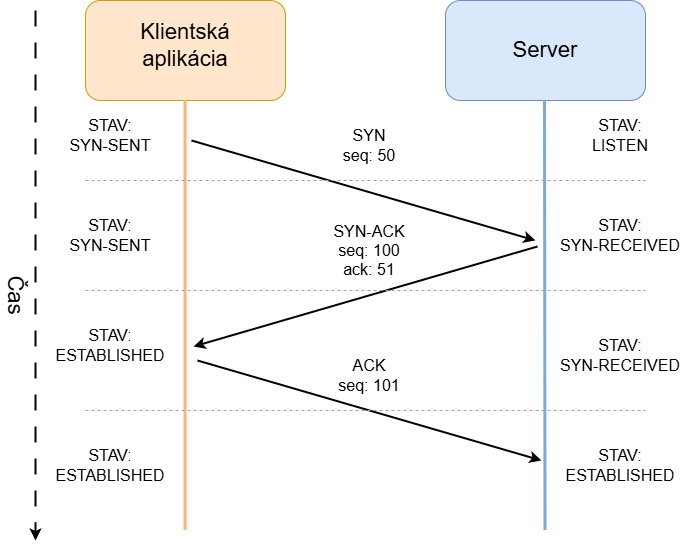
\includegraphics[width=0.6\linewidth]{obrazky-figures/TCPhandshake.png}
    \caption{TCP three-way handshake}
    \label{fig:tcp_handshake}
\end{figure}
Po nadviazaní spojenia TCP zabezpečuje spoľahlivé doručenie dát pomocou už spomínaných sekvenčných čisel 2 typov:
\begin{itemize}
    \item \texttt{seq} (Sequence Number) -- Určuje poradové číslo prvého bajtu dát v~danom segmente v~rámci celého prúdu.
    \item \texttt{ack} (Acknowledgment Number) -- Signalizuje úspešné prijatie dát a~určuje poradové číslo nasledujúceho očakávaného bajtu.
\end{itemize}
Po každom prijatí dát príjmateľ odosiela ACK paket.

\subsection{Segmentácia}
,,Termín segmentácia označuje činnosť, ktorú TCP vykonáva pri~preberaní prúdu bajtov z~odosielajúcej aplikácie a~ich balení do~TCP segmentov''~\cite{rfc9293}. Tento jav je spôsobený limitom prenosu na~fyzickej vrstve sieťovej komunikácie nazývaným \textit{Maximum Transmission Unit} (MTU). Protokol teda musí prenášané dáta rozdeľovať do~segmentov (paketov na~úrovni TCP), pričom sa~ich snaží vytvárať čo najväčšie, aby zefektívnil komunikáciu znížením réžie. V~praxi sa~tak jedna ucelená TLS správa (napr. Client Hello alebo aplikačné dáta) môže rozdeliť do~viacerých TCP paketov. Pri~analýze sieťovej prevádzky sa~potom táto správa nejaví ako jeden celistvý blok, ale ako sekvencia viacerých na~seba nadväzujúcich segmentov.

\subsection{Porty komunikácie}\label{th:ports}
Na identifikáciu konkrétnych sieťových procesov a~aplikácií bežiacich v~rámci zariadenia využíva protokol TCP čísla portov, ktorých využitie je spomenuté nižšie. Klientské aplikácie majú pridelené porty v~rozsahu od~0 do~65535, vďaka ktorým sa~odlišujú od~súbežných aplikáciach na~danom zariadení. Čísla portov môžeme rozdeliť do~nasledujúcich~3 skupín:
\begin{itemize}
    \item \textbf{Dobre známe porty} (0 -- 1023) -- rezervované pre~systémové služby.
    \item \textbf{Registrované porty} (1024 -- 49151) -- vyhradené konkrétnym aplikáciam (veľakrát rozšírené serverové aplikácie)
    \item \textbf{Dynamické porty} -- nepriradené, slúžia pre~zvyšok aplikácií. Tieto čísla sú pridelené zväčša operačným systémom zariadenia.
\end{itemize}

\section{Protokol TLS}
TLS protokol je najpoužívanejší protokol zabezpečujúci bezpečný a~šifrovaný prenos. TLS protokol vznikol ako oficiálna globálne používaná verzia svojho zastaraného predchodcu SSL, z~ktorého sa~vyvinul. Existuje niekoľko verzií protokolu TLS, pričo dnes sú podporované už iba verzia 1.2 a~jej následník 1.3.~\cite{rfc8996}

\subsection{Protokol SSL}
Tento protokol slúžil ako základný stavebný kameň pre~šifrovanú komunikáciu medzi protokolom TCP a~aplikačnými protokolmi. Bol navrhnutý v~90. rokoch spoločnosťou Netscape Communications a~dnes je už nepoužívaný, avšak základné princípy komunikácie či nadviazania spojenia s~ním TLS zdiela. Je navrhnutý ako klient/server protokol, ktorého základným zmyslom bolo poskytnúť nasledujúce služby:~\cite{oppliger2023ssl}
\begin{itemize}
    \item \textbf{Autenticita} -- ,,Proces overovania tvrdenia, že~systémová entita alebo systémový prostriedok má určitú hodnotu atribútu.''~\cite{rfc4949}. Konkrétne SSL/TLS zaisťuje overenie identity nielen na~začiatku pri~nadväzovaní spojenia s~druhým účastníkom komunikácie, ale garantuje aj pravosť všetkých prijatých dát (skutočnosť, že~pochádzajú od~zdroja, s~ktorým komunikujeme).
    
    \item \textbf{Dôvernosť} -- v~zmysle RFC 4949~\cite{rfc4949} ide o službu dôvernosti dát, ktorá zabezpečuje ochranu všetkých používateľských dát prenášaných v~rámci jedného komunikačného spojenia pred~neoprávneným odhalením. Dôvernosť teda znamená, že~k posielaným dátam majú prístup iba povolené entity. Prúd dát sa~považuje za~dôverný, ak každý prenesený paket je zašifrovaný.

    \item \textbf{Integrita} -- tu sa~opäť vzťahuje termín pre~integritu dát, pričom znamená, že~dáta v~aktívnom komunikačnom prúde nemôžu byť úmyselne či náhodne zmenené alebo poškodené~\cite{rfc4949}. SSL/TLS však nezabezpečuje spoľahlivosť prenosu (na to~slúži protokol TCP), ale zaobstaráva detekciu akejkoľvek neoprávnenej manipulácie s~obsahom alebo poradím úspešne doručených správ.
\end{itemize}
Tieto základné služby protokoly SSL a~TLS zdieľajú, rozdiely nastávajú až v~ich výslednom prevedení, ktoré sú popísané nižšie v~sekcii \ref{th:SSL_TLS_diff}.

\subsection{Rozdiely medzi SSL a~TLS}\label{th:SSL_TLS_diff}
Ako bolo už spomenuté, TLS  (vnímaný aj ako SSL verzia 3.1) a~SSL sú dva veľmi príbuzné protokoly, pričom posledná používaná verzia SSL bola 3.0~\cite{rfc7568}. Hlavný rozdiel spočíva v~úrovni bezpečnosti a~použitých algoritmoch pre~jej dosiahnutie.

SSL využívalo pre~zabezpečenie algoritmus/techniku \textbf{MAC} (\textit{Message Authentication Code}). Tento algoritmus využíva bežné kryptografické funkcie ako napríklad \textit{SHA1} alebo \textit{MD5} na~generovanie odtlačku, pričom pri~tvorení hashu spojí obsah správy a~privátny kľúč, keďže hashovacie funkcie bývajú verejne dostupné. Kvôli zníženej bezpečnosti protokol TLS prešiel na~štandardizovaný algoritmus \textbf{HMAC} (\textit{Hash-based Message Authentication Code}). Tento algoritmus využíva MAC konštrukciu s~iteratívnym hashovaním blokov správy, pričom aplikuje vnútornú a~vonkajšiu vrstvu hashovania (tzv. inner a~outer pass) s~využitím modifikovaného tajného kľúča pomocou konštánt~\cite{kim2006security}. Výsledná hashovacia konštrukcia, ktorá využíva HMAC sa~označuje ako \textbf{PRF}\label{th:prf} (pseudonáhodná funkcia), čo znamená, že~útočník nie je schopný rozlíšiť náhodný výsledok od~výsledku tejto funkcie. Týmto eliminuje zraniteľnosť voči útokom (napr. \textit{Length Extension Attack}~\cite{pentesterlab_lea}), ktorým podliehali jednoduché algoritmy využívajúce zastaraný MAC.

Ďalej TLS už nepodporuje prelomené šifrovacie algoritmy ako napríklad \textit{MD5}, ale len tie, ktoré spĺňajú vlastnosť \textbf{Forward secrecy} (dopredné utajenie). Táto vlastnosť je definovaná nasledovne: ,,Zverejnenie súkromných kľúčov niektorých používateľov neohrozuje (sémantickú bezpečnosť) predtým dohodnutých kľúčov.''~\cite{kim2006security} To znamená, že~ak sa~aj útočníkovi podarí získať súkromný kľúč servera, stále nebude môcť dešifrovať predošlú komunikáciu s~klientom (hlavný rozdiel medzi RSA a~Diffie-Hellman).

\subsection{Štruktúra TLS}
Protokol TLS sa~skladá z~2 častí:~\cite{oppliger2023ssl}
\begin{itemize}
    \item Spodná vrstva -- \textit{TLS record protocol} 
    \item Horná vrstva (\textit{TLS Handshaking Protocols}) -- \textit{TLS Change cipher spec protocol} (verzia 1.2), \textit{TLS alert portocol}, \textit{TLS handshake protocol} a~\textit{TLS application data protocol}
\end{itemize}
\textit{TLS record protocol} slúži na~manipuláciu aplikačných dát z~vyšších vrstiev. Jeho hlavnými úlohami sú:
\begin{itemize}
    \item \textbf{Fragmentácia} -- Rozdeľuje dáta na~menšie bloky, tzv. \textit{TLSPlaintext records}, ktoré sú lepšie spracovateľné, pričom maximálna veľkosť jedného je $2^{14}$ bajtov~\cite{rfc5246}.

    \item \textbf{Kompresia} -- Voliteľný krok, pri~ktorom sú záznamy skomprimované pomocou algoritmu, ktorý má každá relácia spojenia. Algoritmus vytvára z~\textit{TLSPlaintext} štruktúry skomprimovanú \textit{TLSCompressed} štruktúru~\cite{rfc5246}.

    \item \textbf{Autentifikácia} -- Pred šifrovaním sa~vypočíta MAC odtlačok, ktorý sa~v~ďalšom kroku priloží k~štruktúre s~dátami~\cite{rfc5246}.

    \item \textbf{Kryptografická ochrana} -- Kryptografické funkcie transformujú \textit{TLSCompressed} štruktúru na~\textit{TLSCiphertext} (zašifrovaný obsah s~MAC odtlačkom)~\cite{rfc5246}. Táto výsledná štruktúra obsahuje okrem zašifrovaných dát aj TLS record hlavičku (\textit{TLS record header}), ktorá obsahuje aj typ správy, verziu protokolu a~dĺžku dát~\cite{oppliger2023ssl}.  
\end{itemize}
\textbf{Horná vrstva} slúži na~logické riadenie relácie a~prenos informácií o aplikácii (metadát), pričom každý pod-protokol definuje svoj vlastný spôsob na~základe jeho využitia:

\begin{itemize}
    \item \textit{Change Cipher Specs protocol} slúži na~signalizáciu zmeny v~dohode o použitých šifrovacích algoritmoch v~komunikácii. Protokol využíva jednu správu od~klienta servera a~je poslaná po~odsúhlasení parametrov pre~šifrovanie medzi komunikantmi~\cite{rfc5246}.
    
    \item \textit{Alert Protocol} slúži na~ohlásenie výnimočnej udalosti. Správy protokolu majú dva typy dôležitosti: varovné a~fatálne. Akonáhle má správa dôležitosť fatálnu, nastáva okamžité prerušenie spojenia~\cite{rfc5246}.
    
    \item \textit{Aplication Data Protocol} je len označenie pre~dáta z~aplikačného protokolu, ktoré nesie record layer~\cite{rfc5246}.
    
    \item \textit{Handshake Protocol} slúži na~dohodu oboch strán komunikácie na~kryptografických parametroch, ktoré sú verzia protokolu, šifrovacie algoritmy a~techniku na~výmenu tajomstva (\textit{secret}) pre~získanie privátnych kľúčov. Význam protokolu spočíva hlavne pre~inicializáciu komunikácie, ktorá je popísaná v~kapitole nižšie ~\ref{th:connection_establishment}. 
\end{itemize}
Celá štruktúra protokolu TLS je vizuálne reprezentovaná na~obrázku \ref{fig:tlsstruct} nižšie, kde tok dát reprezentuje zasielanie správy. Pri~príjmaní správ je tok dát reverzný.

\begin{figure}[H]
    \centering
    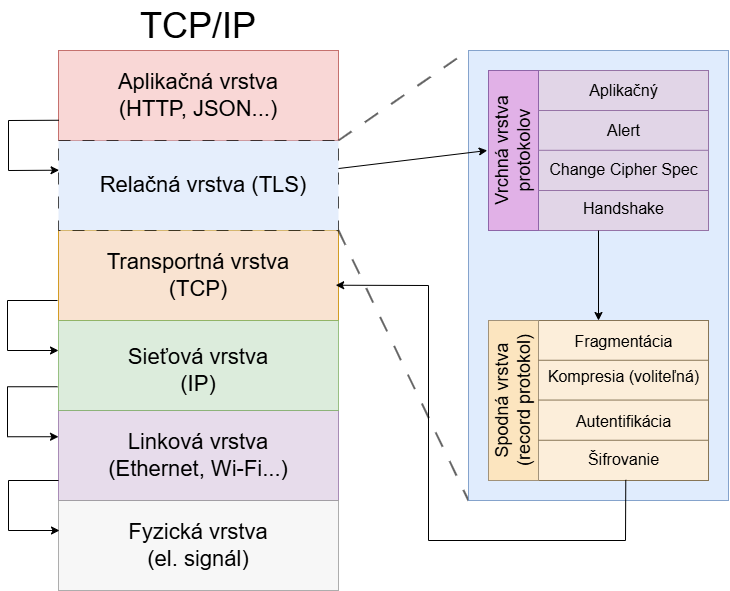
\includegraphics[width=0.6\linewidth]{obrazky-figures/TLSstruct.png}
    \caption{Štruktúra TLS v~rámci modelu TCP/IP}
    \label{fig:tlsstruct}
\end{figure}

\subsection{Nadviazanie spojenia}
\label{th:connection_establishment}
V tejto sekcií je vysvetlený základný princíp inicializácie spojenia definovaného nad protokolom \textit{TLS Handshake Prototcol} a~definície správ protokolu podľa RFC 5246~\cite{rfc5246} dokumentácie, ktorá opisuje najpoužívanejšiu verziu v~dosupnej datovej sade TLS 1.2. 

\subsubsection{Typy správ}\label{message_type}
\begin{itemize}
    \item \textbf{Hello Messages} -- Slúžia na~výmenu informácií o schopnostiach zabezpečenia medzi klientom a~serverom. Pri~začatí novej relácie sú algoritmy šifrovania, hashovania a~kompresie v~stave pripojenia record vrstvy vynulované a~predpokladá sa~na~ich dohode pomocou týchto správ v~\textbf{nešifrovanej} podobe. V~prípade opätovného vyjednávania (renegotiation) sa~správy už neprenášajú otvorene, ale sú chránené aktuálne nastaveným zabezpečením. 
    
    Hello správy majú 3 druhy: 
    \begin{enumerate}
        \item \textbf{\textit{Hello Request}} -- Túto správu posiela server, pričom slúži na~opätovné začatie handshake-u. Klient na~túto správu musí reagovať novou \textit{Client Hello}~(\ref{th:client_hello}) správou.

        \item \textbf{\textit{Client Hello}}\label{th:client_hello} -- Klient posiela túto správu, akonáhle chce inicializovať TLS spojenie so serverom. Obsahuje parametre:
        \begin{itemize}
            \item \textit{Version} -- Najvyššia verzia protokolu TLS.
            
            \item \textit{Random} -- Náhodné číslo vygenerované klientom, slúžiace ako identifikácia unikátnosti spojenia, ktorým sa~zabraňuje k~opakovaní použitých odtlačkov (integritné opatrenie) a~dočasných kľúčov komunikácie~\cite{oppliger2023ssl}.
            
            \item \textit{Session ID} -- Identifikátor relácie, ktorým klient určuje reláciu, ku ktorej sa~chce pripojiť (ak sa~už niekedy k~serveru pripájal, môže využit existujúcu reláciu a~preskočiť handshake).
            
            \item \textbf{\textit{Cipher Suites}}\label{th:cipher_suites} -- Zoznam všetkých kombinácií šifrovacích algoritmov, ktoré klient ovláda, zoradený podľa preferencie.  Šifrovacia sada sa~skladá zo~symetrického algoritmu pre~šifrovanie dát, algoritmu pre~bezpečnú výmenu šifrovacieho kľúča a~typu HMAC algoritmu na~overenie integrity.
            
            \item \textit{Compression Methods} -- Zoznam podporovaných metód kompresie, dnes už väčšinou prázdne kvôli bezpečnosti~\cite{rfc7525}.
            
            \item \textbf{\textit{Extensions}} -- Zoznam podporovaných rozšírení.
        \end{itemize}
        
        Táto správa je dôležitá pre~ďalšiu časť práce, kde sa~využívajú hlavne rozšírenia (viac v~sekcii \hyperref[th:extensions]{Rozšírenia}).

        \item \textbf{\textit{Server Hello}} -- túto správu posiela server ako odpoveď na~\textit{Client Hello}~(\ref{th:client_hello}), pričom jej obsahom je množina rozšírení (extensions) a~šifrovacích algoritmov, ktorú si server vybral od~možností poskytnutých klientom.
    \end{enumerate}

    \item \textbf{Server Certificate} -- tento typ správy posiela server a~slúži na~sprostredkovanie identity klientovi ak ho šifrovacia sada požaduje na~autentifikáciu. Obsahuje digitálny podpis a~verejný kľúč servera a~autorít, ktorého podpísali.

    \item \textbf{Server Key Exchange Message} -- táto správa je voliteľná. Posiela sa~iba vtedy, ak certifikát servera neobsahuje dostatok dát na~to, aby si klient a~server mohli vymeniť \textit{pre-master secret}.

    \item \textbf{Certificate Request} -- zoznam akceptovaných typov certifikátov a~zoznam mien autorít, ktorým server dôveruje. Správa je voliteľná a~posiela sa~iba vtedy, ak  server vyžaduje autentifikáciu klienta.

    \item \textbf{Server Hello Done} -- táto správa neobsahuje žiadne dáta, slúži iba ako signalizácia od~servera na~dokončenie ,,Hello'' fázy (nie celej inicializácie spojenia, správa sa~posiela pred~vznikom kľúčov).

    \item \textbf{Client certificate} -- odpoveď klienta na~\textit{Certificate Request}, ktorá obsahuje certifikát klienta alebo má prázdny obsah.

    \item \textbf{Client Key Exchange Message}\label{th:client_key_exchange} -- správu posiela klient hneď po~prijatí \textit{Server Hello Done} správu, prípadne po~poslaní \textit{Client Certificate}. Obsah správy závisí od~typu algoritmu výmeny kľúčov. Pri~\textbf{RSA} sa~posiela \textit{Pre-Master Secret} zašifrovaný verejným kľúčom servera. Pri~mechanizme \textbf{Diffie-Hellman} sa~posiela \textit{Public Value}, kde na~rozdiel od~RSA sa~\textit{PreMaster Secret} vypočíta na~každej strane, a~teda sa~neposiela cez sieť.

    \item \textbf{Certificate Verify} -- táto správa sa~posiela iba ak klient poslal svoj certifikát serveru. Klient zahashuje všetky doteraz poslané \textit{handshake} správy a~výsledok pošle serveru na~overenie verejným kľúčom certifikátu.

    \item \textbf{Change Cipher Spec} -- posiela klient alebo server a~signalizuje začiatok šifrovanej komunikácie podľa dohodnutých algoritmov a~parametrov šifrovania. Po tejto správe nasleduje správa \textit{Finished}.

    \item \textbf{Finished} -- posiela ju server aj klient na~signalizáciu úspešneho nadviazania spojenia. Toto je zároveň aj prvá šifrovaná správa spojenia. Obsahuje výsledok \hyperref[th:prf]{PRF} funkcie všetkých doterajších správ handshake-u pre~overenie integrity komunikácie.
\end{itemize}

\subsubsection{Rozšírenia}\label{th:extensions}
Rozšírenie je určitý doplnok/modul pre~TLS, ktorý je definovaný ako dvojica \{ \textit{extension\_type, extenstion\_data} \}, kde podľa typu rozšírenia sa~v~dátovej časti ukladá konkrétna dátová štruktúra. Existuje mnoho typov rozšírení, pričom najpoužívanejšie sú:
\begin{itemize}
    \item {SNI}\label{SNI} (\textit{Server Name Indication}) -- Obsahuje konkrétnu doménu servera ku ktorej sa~chce klient pripojiť~\cite{rfc6066}. Toto rozšírenie sa~v~Client Hello správe nachádza pod názvom \textit{Server Name}. 
        
    \item ALPN (\textit{Application-Layer Protocol Negotiation}) -- Obsahuje zoznam podporovaných aplikačných protokolov (napr. HTTP2/HTTP3\dots), z~ktorých si môže server vybrať a~zefektívniť tak nadviazanie komunikácie bez nutnosti ďalších dodatočných sieťových prenosov~\cite{rfc7301}.

    \item \textbf{Podporované skupiny} (\textit{Supported Groups})\label{th:supported_groups} -- Definuje zoznam matematických skupín (najčastejšie eliptických kriviek), ktoré je klient schopný použiť v~rámci algoritmu Diffie-Hellman na~bezpečné nadviazanie spoločného kľúča~\cite{rfc8422}. Tu sa~definujú konkrétne parametre pre~vybraný šifrovací algoritmus zo~cipher suites.

    \item Podpisové algoritmy \textit{(Signature Algorithms)} -- Definuje zoznam podporovaných dvojíc \{ hashovacia\_funkcia, podpisový\_algoritmus \}. Tento zoznam teda ponúka serveru spôsoby, ktorými si dokáže klient overiť jeho digitálny podpis~\cite{rfc5246}.
\end{itemize} 

\subsubsection{TLS Handshake}

TLS handshake začína až vtedy, ak je dokončený TCP Handshake \ref{th:TCPHandshake}. Pri~nadväzovaní spojenia sa~využívajú správy obsiahnuté v~sekcii \hyperref[message_type]{Typy správ}. Priebeh vytvorenia spojenia je vysvetlený podľa publikácie Kuroseho a~Rossa~\cite{kurose_ross_2021}.

\begin{enumerate}
    \item Klient pošle \textit{Client Hello} s~náhodným číslom.
    
    \item Server odpovedá správou \textit{Server Hello}, ktorá obsahuje serverom vybranú šifrovaciu sadu  z~\textit{Client Hello}. Server taktiež posiela svoje náhodné číslo.
    
    \item Server následovne hneď posiela \textit{Server Certificate} správu s~certifikátom servera.
    
    \item Klient si overí cerifikát. V~prípade algoritmu RSA si klient vygenereuje \textit{Pre-Master Secret} (tajné číslo), zašifruje ho verejným kľúčom servera a~pošle serveru. V~dnešnej dobe sa~však častejšie používa bezpečnejší algoritmus Diffie-Hellman, kde sa~posielajú iba verejné parametre algoritmu a~tajné číslo si každá strana vypočíta samostatne. Pre~oba algoritmy posiela klient požadované hodnoty v~správe \textit{\hyperref[th:client_key_exchange]{Client Key Exchange}}. 
    
    \item Obe strany si následne vypočítajú \textit{Master Secret} (MS) kombináciou \textit{Pre-Master Secret} a~oboch náhodných čisel, ktoré si server a~klient vymenili na~začiatku. Vďaka MS sa~vygenerujú privátne kľúče pre~šifrovanie komunikácie a~kontrolu integrity.
    
    \item Klient následne odosiela správy \textit{Change Cipher Spec} a~\textit{Finished} (\hyperref[th:prf]{PRF} všetkých doterajších správ)~\cite{rfc5246}.  
    
    \item Server taktiež odosiela správy \textit{Change Cipher Spec} a~\textit{Finished}.

    \item Ak obe strany úspešne overia obsah \textit{Finished správ}, handshake je dokončený a~kanál je pripravený na~šifrovaný prenos dát.
\end{enumerate}

Celý proces je vizuálne zobrazený na~obrázku nižšie.~\ref{fig:TLShandshake}

\subsection{TLS 1.3}
Verzia 1.2 sa~dlhodobo považovala za~štandard a~v~súčasnosti stále predstavuje významnú časť sieťovej prevádzky, najmä kvôli spätnej kompatibilite so staršími zariadeniami. Do popredia sa~však čoraz výraznejšie dostáva modernejšia verzia 1.3, ktorá ma rozdiely definované v~RFC 8446~\cite{rfc8446}:
\begin{itemize}
    \item \textbf{Filtrácia zastaraných algoritmov} -- V~TLS 1.2 a~starších verziách bolo povolených množstvo šifier, ktoré sa~časom ukázali ako problematické, a~teda TLS 1.3 tieto algoritmy odmietol a~zostali iba algoritmy spĺňajúce vlastnosť AEAD (\textit{Authenticated Encryption with Associated Data}). Tieto algoritmy zaisťujú nemennosť viditeľných parametrov (napríklad hlavička record vrstvy) tým, že~ich použijú pri~výpočte autentifikačneého odtlačku.

    \item \textbf{Znížený RTT} (\textit{round-trip time}) -- Pri~prvom pripojení vyžaduje len 1-RTT (jednu vzájomnú výmenu správ), pretože klient posiela svoje podklady (\textit{Key Shares}) už v~úvodnej správe \textit{Client Hello}. Okrem toho zavádza režim 0-RTT (\textit{Zero Round-Trip Time Resumption}), ktorý umožňuje klientovi poslať šifrované aplikačné dáta okamžite v~prvom pakete za~predpokladu, že~strany využijú informácie z~predchádzajúcej relácie (tzv. \textit{Pre-Shared Key}).

    \item \textbf{Zvýšené súkromie} -- Všetky správy po~\textit{Server Hello} sú vo~verzii 1.3 šifrované.

    \item \textbf{Odstránenie \textit{Change Cipher Spec}} – Keďže sa~v~TLS 1.3 parametre potrebné na~odvodenie kľúčov posielajú už v~správach \textit{Client Hello} a~\textit{Server Hello}, protokol dokáže prejsť na~šifrovanú komunikáciu okamžite a~automaticky. Na~rozdiel od~starších verzií definuje TLS 1.3 striktné poradie správ, čím sa~správa \textit{Change Cipher Spec} stáva nadbytočnou.
\end{itemize}

\begin{figure}[H]
    \centering
    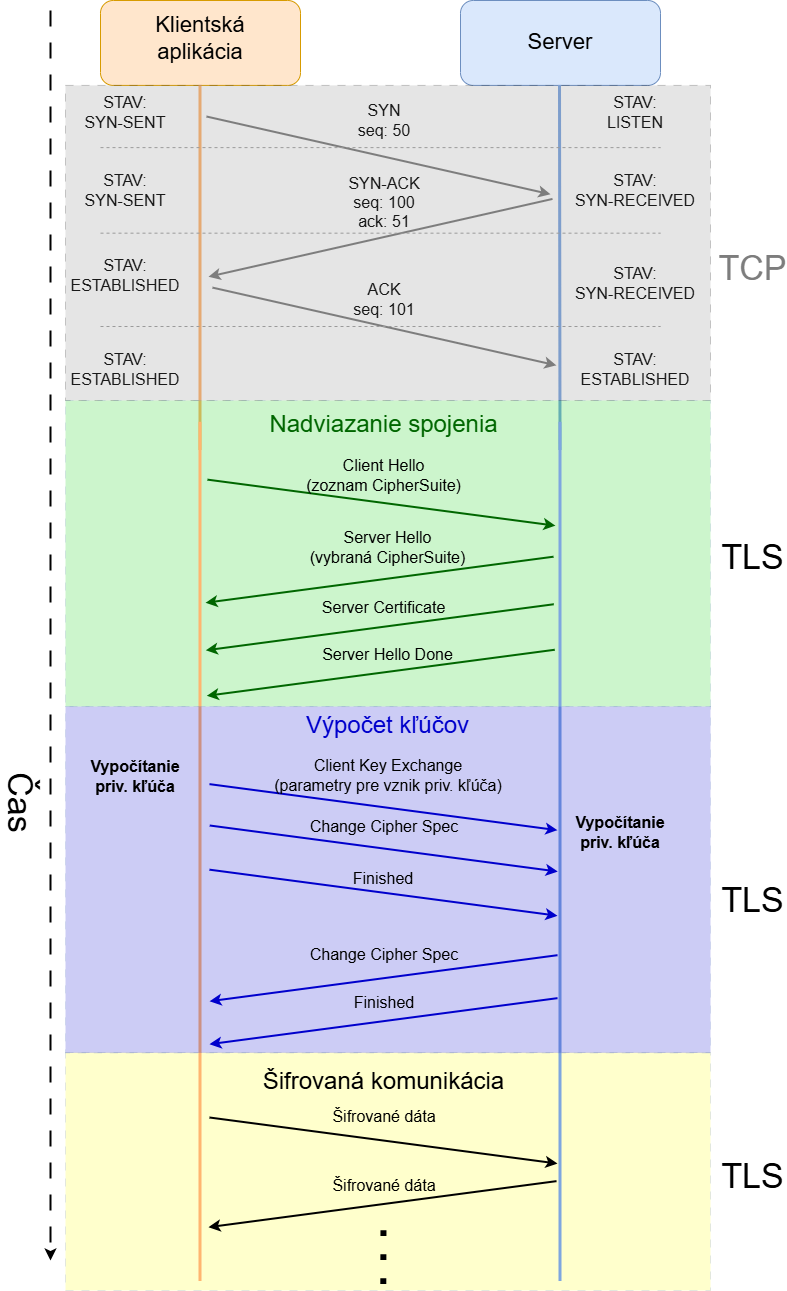
\includegraphics[width=0.7\linewidth]{obrazky-figures/TLSHandshake.png}
    \caption{Celý proces nadväzovania TLS komunikácie}
    \label{fig:TLShandshake}
\end{figure}

\chapter{Autoenkodéry}
Táto kapitola sa~zaoberá teoretickým popisom autenkodérových sietí, ktoré boli implementované za~účelom identifikácie aplikácií. Kapitola rozoberá základy neurónových sietí potrebné pre~pochopenie princípu autoenkodérov. Následne sú vysvetlené princípy práve tohoto typu neurónovej siete, odlišnosti medzi jednotlivými druhmi a~spôsoby ich trénovania na~extrakciu kľúčových príznakov zo~šifrovanej sieťovej prevádzky.

\section{Autoenkodéry ako neurónové siete}
Autoenkodéry sú špecifickým typom neurónových sietí, ktoré transformujú numerické dáta na~vstupe špecifickou kompresiou do~zúženého priestoru (latentného priestoru) a~následne rekonštruujú vstup len na~základe tohoto priestoru s~cieľom čo najmenšej straty informácií. Myšlienkou tohoto procesu je vyťaženie kritických a~najpodstatnejších informácií z~dát bez potreby rozsiahleho ľudského dohľadu (\textit{unsupervised learning}~\ref{th:unsupervised})~\cite{mienye2025deep}.

\subsection{Definícia a~rámec strojového učenia}
Popis tejto sekcie vychádza z~publikácie \textit{Deep Learning} od~Goodfellowa a~kol.~\cite{Goodfellow-et-al-2016} Strojové učenie nám prináša možnosť pre~riešenie problémov, ktoré sú príliš ťažké na~to, aby ich riešili programy navrhnuté ľuďmi. Každý model využíva nejaký \textbf{učiaci algoritmus}, ktorý má základnú štruktúru:
\begin{itemize}
    \item Vykonáva určitú \textbf{úlohu} -- v~našom prípade klasifikácia aplikácií.
    \item Meria svoj \textbf{výkon} -- úspešnosť vykonávania úlohy so zameraním na~nejaký parameter (\textit{Accuracy}, \textit{F1 score}, \textit{Recall} \dots).
    \item Zlepšuje (učí) sa~na~základe \textbf{skúseností} -- skúsenosti sú reprezentované trénovacími dátami, v~ktorých sa~modely snažia hľadať kľúčové príznaky a~súvislosti pre~vyriešenie daného problému. Existujú 2 druhy učenia: \textit{\textbf{Supervised}} (každým dátam je priradený štítok s~očakávaným výsledkom pre~danú vzorku) a~\textit{\textbf{Unsupervised}} (dáta sú neoznačené, model musí sám nájsť súvislosť)\label{th:unsupervised}.
\end{itemize}
\label{training_basics}Hlavným účelom učiaceho algoritmu je, aby natrénoval model do~stavu, kedy vie rozlíšiť nie len trénovacie dáta, ale aj nový vstup, ktorý ešte doteraz nevidel. Táto vlastnosť sa~označuje ako \textbf{generalizácia}\label{th:generalisation}. Pri~trénovaní modelov sa~teda snažíme dosiahnuť čo najmenšiu trénovaciu a~testovaciu chybu. Tu sa~stretávame s~2 častými problémami pri~strojovom učení:
\begin{itemize}
    \item \textbf{\textit{Underfitting}} (Podučenie) -- K tomuto javu dochádza, ak model nie je schopný dosiahnuť dostatočne nízku trénovaciu a~testovaciu chybu. Model je teda príliš jednoduchý vzhľadom na~trénovaciu sadu dát.
    \item \textbf{\textit{Overfitting}}\label{th:overfitting} (Preučenie) -- K tomuto javu dochádza, ak má model veľký rozdiel chybovosti medzi trénovaciu chybou (nízka) a~testovaciou chybou (vysoká). Model býva v~takomto prípade príliš komplexný vzhľadom na~trénovaciu sadu dát.
\end{itemize}
Na čo najlepšiu generalizáciu a~predchádzanie \textit{overfittingu} alebo \textit{underfittingu} sa~manipuluje s~modelovou \textbf{kapacitou}. Kapacita\label{th:capacity} modelu vyjadruje schopnosť hypotetického priestoru (množiny všetkých funkcií, ktoré sa~model môže naučiť) aproximovať rôzne typy matematických vzťahov v~dátach. Teoretický cieľ je dosiahnuť \textbf{reprezentačnú} kapacitu modelu, ktorá hovorí o tom, aké zložité funkcie by sieť teoreticky mohla vypočítať, ak by sa~model učil dokonalým algoritmom. Optimalizačný algoritmus však nedokáže nájsť v~konečnom čase najlepšie riešenie, ale sa~k~nemu iba približuje, a~teda v~praxi sme schopní dosiahnuť len tzv. \textbf{efektívnu} kapacitu, ktorá sa~líši od~ideálneho stavu.

\subsection{Štruktúra neurónových sietí}
Popis tejto sekcie taží taktiež z~publikácie \textit{Deep Learning} od~Goodfellowa a~kol.~\cite{Goodfellow-et-al-2016} Pojem neurónová sieť vychádza z~neurovedy, kde komplexný systém (mozog) je tvorený malými jednotkami (neurónmi), ktoré spolu komunikujú pomocou elektrických impulzov. \textbf{Neurón} tu predstavuje matematickú jednotku, ktorá prijíma vstupy, spracováva ich a~generuje výstup. V~technickom zmysle je neurón vnímaný ako skalárna funkcia, ktorá transformuje vstupný vektor na~jednu číselnú hodnotu. V~strojovom učení sa~snažíme priblížiť k~tomuto konceptu pomocou aproximačných funkcií, ktoré sú navrhnuté, aby dosiahli štatistickú \hyperref[th:generalisation]{generalizáciu}. 

Model sa~skladá z~\textbf{vrstiev}, kde jedna vrstva modelu predstavuje zoskupenie neurónov (reprezentované vektorom), ktoré pracujú paralelne, pričom každý z~nich možno interpretovať ako samostatnú výpočtovú jednotku reprezentujúcu funkciu transformujúcu vektorový vstup na~skalárnu hodnotu. Každá vrstva má určitú \textbf{šírku} (dimenziu), ktorá je definovaná ako počet neurónov, ktoré sa~v~nej nachádzajú. Vrstvy modelu sa~typicky radia hierarchicky za~sebou, kde výstup z~predchádzajúcej vrstvy slúži ako vstup pre~nadchádzajúcu vrstvu. Počet vrstiev udáva hĺbku modelu. Vrstva na~úplnom začiatku sa~nazýva vstupná a~na úplnom konci zoradenia je výstupná vrstva. Všetky vrstvy, ktoré sa~nachádzajú medzi nimi, sa~nazývajú skryté (\textit{hidden layers}).

Tento typ usporiadania reprezentuje \textbf{dopredné (\textit{feedforward}) neurónové siete}\label{th:feedforward}, ktorých špecifickou podskupinou sú aj autoenkódery. Cieľom týchto sietí je transformovať vstupný vektor dát na~požadovaný výstup, pričom výstup zo~skrytých vrstiev nie je jasne definovaný trénovacími dátami. Úlohou modelu je v~procese učenia správne optimalizovať vnútorné parametre (váhy a~biasy) tak, aby došlo k~čo najpresnejšej reprezentácii požadovaného výstupu v~poslednej vrstve siete.

\subsection{Princípy trénovania neurónových sietí}
Všeobecné základy pre~neurónové siete v~tejto sekcii opäť vychádzajú z~publikácie \textit{Deep Learning} od~Goodfellowa a~kol.~\cite{Goodfellow-et-al-2016} Ako bolo už spomenuté, neurónová sieť je tvorená pomocou neurónov usporiadaných vo~vrstvách, kde každý neurón je reprezntovaný ako predpis nejakej funkcie, ktorá má všeobecne tvar:
\begin{equation}
    f(x) = w \cdot x + b
\end{equation}
\begin{itemize}
    \item $x$ -- Vstupný vektor dát.
    \item $w$ -- Váhy pre~každý atribút (súradnicu vektora) vstupných dát.
    \item $b$ -- Posun (bias), skalár.
\end{itemize}
Všetky vektory majú dimenziu danú podľa dimenzie vstupných dát. Každý vektor vypočíta skalárny súčin pre~vstup $x$ so svojimi váhami $w$ a~pripočíta bias. Výsledok je jedno čislo (skalár), ktorý sa~posúva ako vstup pre~ďaľšiu vrstvu.
Takto fungujú neuróny v~každej vrstve modelu, a~teda rovnicu pre~celú jednu vrstvu môžeme vyjadriť ako:
\begin{equation}
    h(x) = q(W^T\cdot x + B)
\end{equation}
\begin{itemize}
    \item $W$ -- Matica váh pre~všetky neuróny vo~vrstve.
    \item $B$ -- Vektor biasov neurónov.
    \item $q$ -- Aktivačná funkcia. Aktivačná funkcia predstavuje nelineárnu transformáciu, ktorá sa~aplikuje na~výstup afinných operácií v~každom neuróne. Jej hlavnou úlohou je vniesť do~modelu nelinearitu, čo umožňuje sieti učiť sa~a~reprezentovať zložité vzťahy v~dátach.
\end{itemize}
Základná myšlienka trénovania neurónových sietí spočíva v~tom, že~nepoznáme presný predpis funkcie každej vrstvy, ktoré opisujú požadovaný výsledok, ale iba ho \textbf{iteračne} aproximujeme pomocou modifikácie parametrov $W$ a~$B$. Toto vykonávame pomocou tzv. \textbf{optimalizácie} pri~učení.

\subsubsection{Stratová funkcia (\textit{Loss function})}
Stratová funkcia (inak nazývaná aj \textit{cost} alebo \textit{error function}) kvantifikuje mieru chyby, ktorej sa~model dopustí pri~spracovaní trénovacích dát vzhľadom na~stanovený cieľ (tu klasifikáciu). V~praxi väčšinou nevyhovuje presne úlohe modelu, takže problém, ktorý model rieši, sa~optimalizuje nepriamo. Cieľom trénovacieho algoritmu je iteratívne nájsť takú konfiguráciu parametrov (váh a~biasov), ktorá minimalizuje hodnotu nákladovej funkcie v~celom trénovacom datasete.

\subsubsection{Gradient}
,,Gradient je zovšeobecnením pojmu derivácie pre~funkcie s~viacerými premennými (vektormi). Ak máme funkciu f, ktorej vstupom je vektor x, potom jej gradient je vektor obsahujúci všetky parciálne derivácie tejto funkcie podľa jednotlivých zložiek vektora x.''~\cite{Goodfellow-et-al-2016} Gradient má v~strojovom učení veľký význam, pretože udáva smer zmeny, ktorým ovplyvníme výsledok stratovej funkcie \textbf{najviac}, a~teda sme vďaka nemu schopní určiť, akým spôsobom optimalizovať váhy a~biasy vo~vrstvách modelu. 

Na výpočet gradientov neurónov sa~využíva technika nazývaná \textbf{\textit{backpropagation}}\label{th:backpropagation}. Táto technika funguje na~základe \textbf{reťazového pravidla}, ktoré hovorí, že~ak je daná funkcia $ y = g(x) $ a~od nej závislá funkcia $ z~= f(y) $, tak potom derivácia $z$ podľa $x$ sa~dá zapísať ako:
\begin{equation}
    \frac{dz}{dx} = \frac{dz}{dy} \cdot \frac{dy}{dx}
\end{equation}
Práve týmto spôsobom dokážeme vypočítať podiel na~zmene neurónov postupne od~\textbf{stratovej funkcie} (vychádza z~nej každá derivácia) cez poslednú a~skryté vrstvy až po~vstupnú (prvú) vrstvu. 

\subsubsection{Optimalizácia}\label{th:optim}
Akonáhle model pozná gradient pri~aktuálnej vykonanej úlohe, dokáže upravovať parametre svojich vrstiev.
\begin{equation}
    x' = x - \epsilon \cdot \nabla_xf(x)
\end{equation}
\begin{itemize}
    \item $x$ -- Vektor pre~váhy v~danej vrstve.
    \item $x'$ -- Nový optimalizovaný vektor pre~váhy v~danej vrstve.
    \item $\epsilon$ -- \textbf{\textit{learning rate}} -- Rýchlosť kroku, akou chceme meniť parametry jednotlivých neurónov.
    \item $\nabla_xf(x)$ -- Vektor gradientu nákladovej funkcie vzhľadom na~parametre x.
\end{itemize}
Tento základný optimalizačný algoritmus sa~označuje ako \textbf{\textit{Stochastic gradient descent}} (SGD)\label{th:sgd}. Hlavným princípom SGD je, že~mení váhy a~biasy vrstiev modelu opačným smerom ako je smer gradientu \textit{loss} funkcie, čím sa~efektívne snaží dosiahnuť jej minimum. Dôležitými premennými pre~stabilitu a~efektivitu učenia sú aj \textit{learning rate} a~\textit{batch size} (veľkosť dávky). Menšia \textit{learning rate} môže viesť k~pomalej konvergencii, zatiaľ čo príliš veľká môže spôsobiť osciláciu \textit{loss} funkcie, niekedy aj divergenciu. \textit{Batch size} udáva počet trénovacích vzoriek/dát, ktoré sú spracované a~je pre~ne vypočítaný gradient v~\textbf{jednom kroku}. Väčšia veľkosť dávky môže zaistiť presnejší gradient, no stáva sa~zložitejším na~výpočet~\cite{mienye2025deep}. Celý proces je možné vidieť na~obrázku \ref{fig:LR_Gradient} nižšie, kde je uvedený jednoduchý príklad neurónovej siete. Sieť najskôr vykoná úlohu na~trénovacích dátach a~vypočíta chybu. Ďalej pomocou \textit{backpropagation} vypočíta postupne všetky gradienty (vychadzajúc z~predpisu stratovej funkcie $L(y)$). Nakoniec optimalizátor aktualizuje váhy $w$ reverzným smerom ako je smer gradientu s~\textit{learning rate} $\eta$.
\begin{figure}[H]
    \centering
    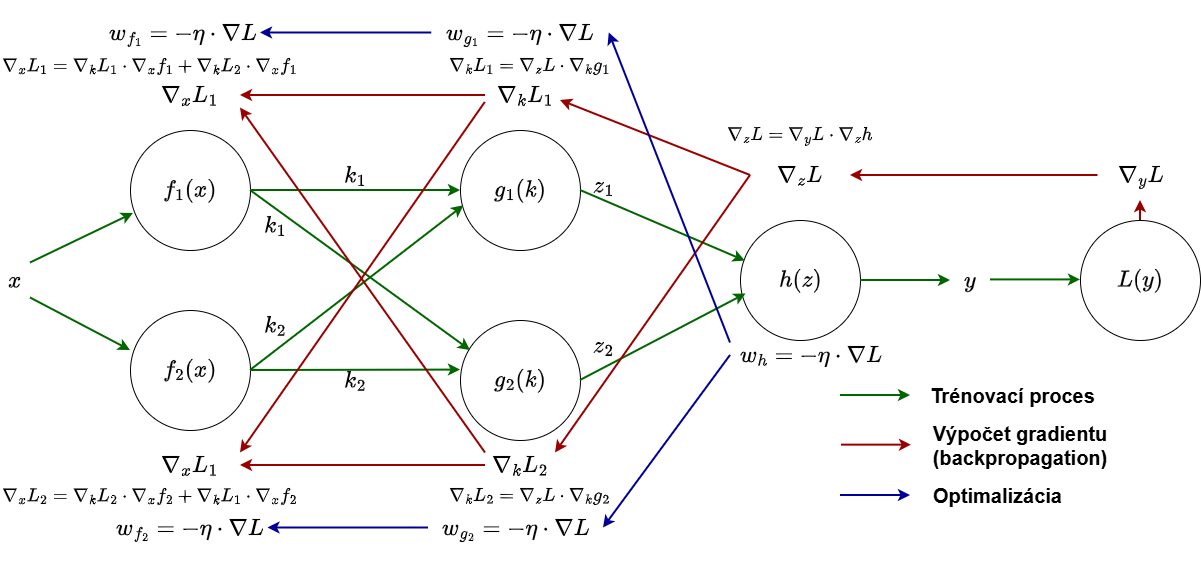
\includegraphics[width=0.9\linewidth]{obrazky-figures/LearningGradient.png}
    \caption{Proces trénovania neorónových sietí.}
    \label{fig:LR_Gradient}
\end{figure}

\subsection{Aktivačné funkcie}
Jednotlivé vrstvy modelu sú definované ako lineárne transformácie vstupov z~predchádzajúcej vrstvy. Bez ďalších transformácií by~bol takýto model schopný aproximovať iba~lineárne vzťahy. Z~tohto dôvodu sa do~architektúry vkladajú aktivačné funkcie s~\textbf{nelineárnym} predpisom, ktoré sieti umožňujú učiť sa~reprezentovať zložitejšie závislosti v~dátach~\cite{Goodfellow-et-al-2016}. Najznámejšia aktivačná funkcia je ReLU (\textit{Rectified Linear Unit}), ktorá má predpis $g(z) = max\{0,z\}$, kde $z$ reprezentuje výstup z lineárnej vrstvy modelu. Táto funkcia teda nuluje všetky záporné výsledky. Ďalšími funkciami sú napríklad Sigmoid: $\sigma(x) = \frac{1}{1+e^{-x}}$. Táto funkica stláča vstup do~intervalu $(0,1)$. Ďalšia známa funkcia je~$tanh(x) = \frac{e^x - e^{-x}}{e^x+e^{-x}}$, ktorá transformuje vstup do~rozsahu $(-1,1)$.

\section{Štruktúra autoenkodérov}
Autoenkodéry, ako už bolo spomenuté v~sekcii \ref{th:feedforward}, sú druh \textit{feedforward} neurónových sietí. Sú špeciálne vďaka svojmu unikátnemu usporiadaniu vrstiev, ktorého cieĺom je dosiahnuť extrakciu kľučových príznakov vstupných dát, vďaka ktorým ich model bude schopný čo najpresnejšie reprezentovať a~rekonštruovať. Táto reprezentácia je vyjadrená ako \textbf{latentný priestor} (\textit{bottleneck}) autoenkodéru, ktorý obsahuje transformované (zakódované) vstupné dáta. \textit{Bottleneck} má typicky najmenšiu dimenziu zo~všetkých vrstiev. Dáta sa~transformujú pomocou \textbf{enkodéra} a~spätne rekonštruujú pomocou \textbf{dekodéra}, ktoré sú tvorené skrytými vrstvami modelu. Enkodér má väčší vstup ako výstup, zatiaľ čo dekodér má dimenzie zrkadlovo opačne~\cite{mienye2025deep}. Schéma je ilustrovaná na~obrázku \ref{fig:autoencoders} nižšie. Na~obrázku je zobrazené, že~dimenzie vstupných vektorov pre~funkcie sú typicky dané nasledovne: $n > m > k$. Vektor $x_1$ až $x_n$ predstavuje vstupné dáta, vektor $b_1$ až $b_k$ predstavuje latentný vektor pre~daný vstup a~vektor $x'_1$ až $x'_n$ zrekonštruovaný výstup. 


\begin{figure}[H]
    \centering
    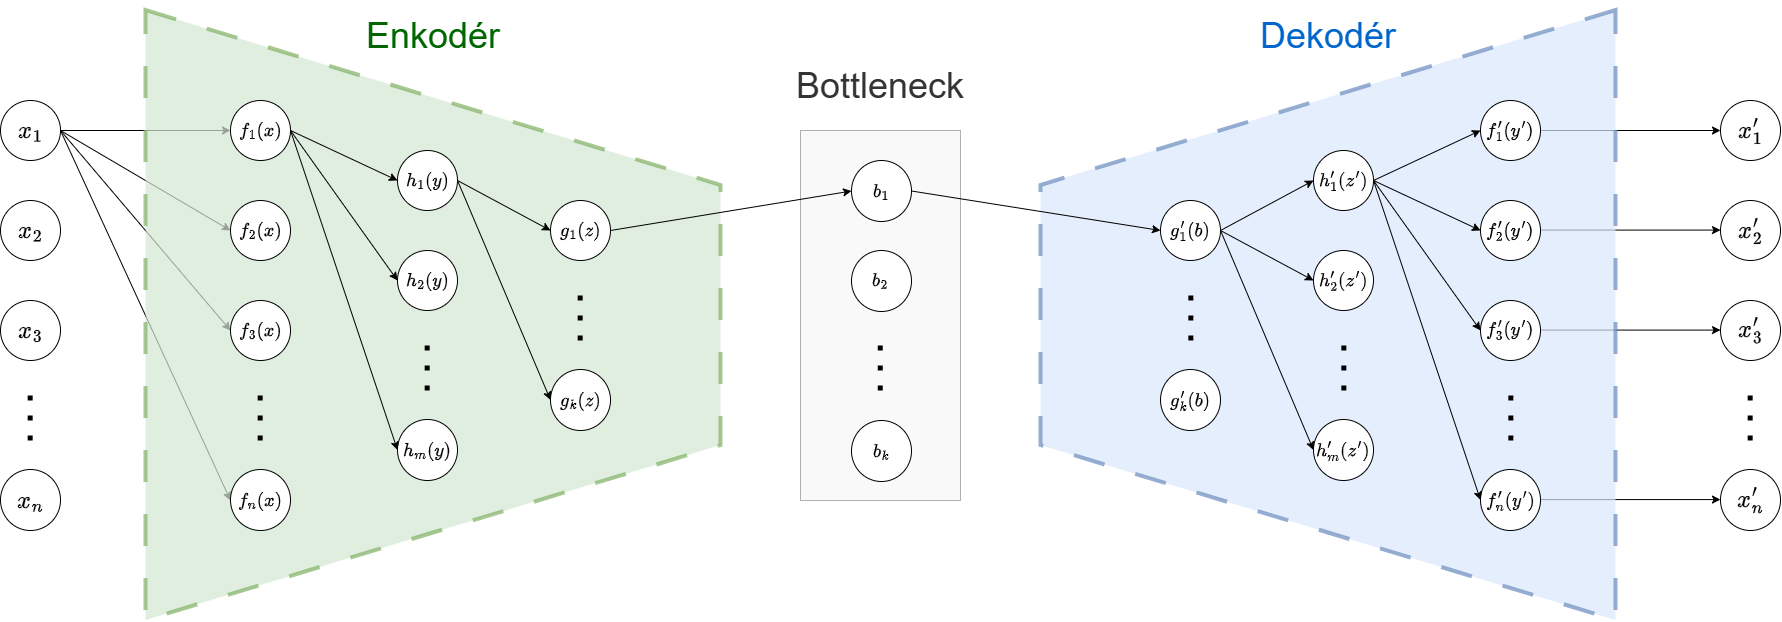
\includegraphics[width=0.95\linewidth]{obrazky-figures/Autoencoders.png}
    \caption{Typická štruktúra autoenkodéru}
    \label{fig:autoencoders}
\end{figure}

\section{Stratová funkcia autoenkodérov}\label{th:MSE}
Keďže autoenkodéry sa~snažia minimalizovať rozdiel medzi vstupným a~výstupným vektorom vo~všetkých súradniciach, často používaná stratová funkcia pre~dáta nebinárneho tvaru je \textbf{MSE} (\textit{Mean Squared Error}). Táto funkcia sa~dá popísať predpisom:
\begin{equation}
    L(\phi,\psi) = \frac{1}{n} \sum^n_{i=1}||x^i - \psi(\phi(x^i)||^2
\end{equation}
pričom $x^i$ je vstupný \textit{i}-ty vektor z~trénovacej dátovej sady, $\phi$ predstavuje funkciu enkodéra a~$\psi$ predstavuje funkciu dekodéra (funkciou sa~tu myslí transformácia cez všetky vrstvy enkodéra/dekodéra)~\cite{mienye2025deep}.

MSE nám pomáha vyzdvihnúť väčšie chyby v~súradniciach vektora od~menších práve vďaka 2. mocnine vo~vzorci. Taktiež poskytuje ľahký výpočet gradientov pri~optimalizácii, pretože funkcia MSE je spojitá~\cite{Goodfellow-et-al-2016}.



\section{Optimalizácia autoenkodérov}
Výpočet gradientu spočíva tak ako aj pri~všeobecných \textit{feedforward} neurónových sieťach z~techniky \textit{backpropagation} (sekcia \ref{th:backpropagation}), pričom sa~využíva v~SGD (sekcia \ref{th:sgd}). SGD je síce základ optimalizačných algoritmov, avšak v~moderných architektúrach sa~často využívajú špecifickejšie algoritmy, konkrétne s~adaptívnymi rýchlosťami učenia (\textit{learning rates}), čo klasický SGD neposkytuje. Medzi najznámejšie patrí algoritmus \textbf{Adam}\label{th:Adam}, ktorý bol použitý aj v~tejto práci.

Názov ,,Adam'' vychádza z~frázy ,,\textit{Adaptive Moment Estimation}'', čo znamená, že~sa počas aktualizovania váh vrstiev modelu prispôsobuje aktuálnym gradientom a~dynamicky mení váhy a~biasy. Toto dokáže na~základe tzv. pamäte. Adam si okrem aktuálneho gradientu uchováva aj informáciu o \textbf{priemere} (zotrvačnosti) a~\textbf{neistote} gradientov (variancii) pomocou 2 parametrov (momentov). Reyad a~kol. vo~svojej štúdii~\cite{reyad2023modified} opisujú algoritmus nasledovne:

\begin{itemize}
    \item $m_t$ -- 1. moment v~časovom kroku $t$, ktorý predstavuje priemer gradientov. Pomáha algoritmu udržiavať smer (zabezpečuje vplyv \textbf{všetkých} doposiaľ vypočítaných gradientov na~výpočet ďalšieho). Dá sa~vyjadriť:
        \begin{equation}
            m_t = \beta_1m_{t-1} + (1 - \beta_1)g_t
        \end{equation}
    \item $v_t$ -- 2. moment v~časovom kroku $t$, ktorý predstavuje rozptyl gradientov. Pomáha znížiť prudké oscilovanie gradientov (nestabilitu). Dá sa~vyjadriť:
        \begin{equation}
            v_t = \beta_2v_{t-1} + (1 - \beta_2)g_t^2
        \end{equation}
\end{itemize}
Pri prechádzaní jednotlivých neurónov sa~krok definuje premennou \textit{t}. Hyperparametre $\beta_1$ a~$\beta_2$ udávajú pomer vplyvu medzi aktuálnym a~predošlými gradientmi na~výpočet nasledujúceho. Premenná $g_t$ označuje súčastný gradient. 

Ďalej sa~vykoná korekcia vychýlenia z~inicializácie algoritmu, aby hodnoty neboli zo~začiatku príliš malé:
\begin{equation}
    \hat{m}_t = \frac{m_t}{1-\beta^t_1},~ \hat{v}_t = \frac{v_t}{1 - \beta^t_2}
\end{equation}
Finálne algoritmus optimalizuje váhy nasledujúcim spôsobom:
\begin{equation}
    \theta_{t+1} = \theta_t - \frac{\eta}{\sqrt{\hat{v}_t}+\epsilon} \hat{m}_t
\end{equation}
kde:
\begin{itemize}
    \item $\epsilon$ -- Malé číslo slúžiace iba proti delení 0.
    \item $\eta$ -- \textit{learning rate}.
    \item $\theta_t$ -- Aktuálna váha vrstvy.
    \item $\theta_{t+1}$ -- Nasledujúca váha vrstvy.
    \item $\hat{m}_t$ -- Smer zmeny váhy.
    \item $\hat{v}_t$ -- Adaptívny škálovací faktor, ktorý bráni oscilovaniu váh.
\end{itemize}
Týmto spôsobom adam zaistí efektívnejšiu a~chytrejšiu optimalizáciu váh, ktorá je menej citlivá na~nevhodné nastavenie počiatočných hyperparametrov v~porovnaní s~klasickým SGD.

\section{Základné typy autoenkodérov}\label{th:autoencoder_types}
Architektúra autoenkodéra je modulárna a~jej modifikáciou je možné dosiahnuť rôzne správanie modelu. Zatiaľ čo klasický poddimenzovaný (\textit{undercomplete}) autoenkodér využíva na~extrakciu čŕt úzke hrdlo, iné varianty využívajú regularizáciu, pridávanie šumu alebo pravdepodobnostné prístupy. Existuje mnoho typov autoenkodérov, pričom táto kapitola opíše iba pár základných, z~ktorých sa~v~tejto práci vyberalo.

\subsection{Undercomplete autoencoders}
Tento typ autoenkodéru je najzákladnejšia forma. Základná myšlienka je prinútiť model učiť sa~iba užitočné informácie, pričom skrytý priestor má menší rozmer ako vstup (\textit{undercomplete} znamená, že~\textit{bottleneck} je menší ako vstup). Proces učenia je definovaný ako minimalizácia stratovej funkcie $L(x,g(f(x)))$, ktorá penalizuje dekodér $g$ a~enkodér $f$ za~akúkoľvek odchýlku zrekonštruovaného výstupu od~pôvodného vstupu. Kľúčovým aspektom pri~návrhu tejto architektúry je voľba kapacity modelu. Ak by bol enkodér alebo dekodér príliš komplexný, model by sa~mohol naučiť reprodukovať vstup bez extrakcie užitočných vlastností distribúcie dát (\textit{overfitting}, sekcia \ref{th:overfitting})~\cite{Goodfellow-et-al-2016}.

\subsection{Sparse autoencoders}
Tento typ autoenkodéra je popísaný na~základe štúdie Mienye a~Swarta~\cite{mienye2025deep}. Sparse autoenkodér pracuje na~princípe \textbf{riedkosti} (\textit{sparse}) aktivovaných neurónov. Hlavným cieľom je prinútiť sieť, aby každý neurón reagoval len na~veľmi špecifický vzor v~dátach. Na~rozdiel od~základného autoenkodéra sa~tu nemení len architektúra, ale upravuje sa~stratová funkcia (Loss function). Pridáva sa~do~nej tzv. trest za~aktivitu, ktorý sa~dá popísať rovnicou:
\begin{equation}
    L_{sparse} = L + \beta \sum_k KL(\rho || \hat{\rho}_k)
\end{equation}
Tu sa~využíva práve \textbf{Kullback-Leiblerova (KL) divergencia}, ktorá porovnáva reálnu pravdepodobnostnú aktivitu neurónov ($\hat{\rho}$) s~požadovanou pravdepodobnosťou $\rho$. Týmto dosiahneme výrazné stúpanie chyby pri~aktivovaní viacerých neurónov, pričom váhu sme schopný regulovať parametrom $\beta$.

\subsection{Denoising autoencoders}
Ako uvádzajú Mienye a~Swart~\cite{mienye2025deep}, tento typ autoenkodéra sa~namiesto učenia na~čistých vstupných dátach učí rekonštruovať čistý výstup z~ich poškodenej verzie. Pred vstupom do~siete sa~dáta upravia tzv. \textbf{korupčnou funkciou} (napríklad pridaním Gaussovho šumu, maskovaním čŕt alebo šumom typu \textit{salt-and-pepper}). Takto upravené dáta vstupujú do~siete a~od autoenkodéra sa~očakáva, že~dokáže tieto chyby opraviť a~zrekonštruovať pôvodný originál. Týmto spôsobom sa~model učí ignorovať irelevantný šum a~sústredí sa~na~extrakciu významných štruktúr v~dátach.

\subsection{Variational autoencoders}
Tento typ autoenkodérov taktiež vychádza zo~štúdie od~Mienyeho a~Swarta~\cite{mienye2025deep}.
Na rozdiel od~\textbf{deterministických} modelov, ktoré boli spomenuté skôr, \textbf{generatívne} modely (ako aj variačný autoenkodér -- VAE) sa~neučia konkrétny výstup, ale vytvárajú (generujú) možných výstupov. Pri~VAE to~je pravdepodobnosť \textbf{normálneho rozdelenia}. VAE sa~teda učí zo~vstupu pomocou enkodéra vytvoriť strednú hodnotu a~rozptyl. Dekodér dostane na~vstup náhodný bod z~tohoto rozdelenia, ktorý rekonštruuje, a~teda dokáže vytvoriť nové dáta podobné pôvodným.

Chyba VAE sa~počíta pomocou konceptu \textbf{ELBO} (\textit{Evidence Lower Bound}, ktorý môžeme vyjadriť nasledovne: 
\begin{equation}
    \mathcal{L}(\theta, \phi; \mathbf{x}) = 
    \mathbb{E}_{q_\phi(\mathbf{z}|\mathbf{x})} [\log p_\theta(\mathbf{x}|\mathbf{z})] 
    - 
    D_{KL}(q_\phi(\mathbf{z}|\mathbf{x}) \parallel p(\mathbf{z}))
\end{equation}
pričom: 
\begin{itemize}
    \item $\mathbb{E}_{q_\phi(\mathbf{z}|\mathbf{x})} [\log p_\theta(\mathbf{x}|\mathbf{z})]$ -- Očakávaná logaritmická vierohodnosť. Udáva mieru, ako dobre dokáže dekodér zrekonštruovať pôvodný vstup zo~\textbf{vzorky} z~latentného priestoru.
    \item $D_{KL}(q_\phi(\mathbf{z}|\mathbf{x}) \parallel p(\mathbf{z}))$ -- KL divergencia. Meria rozdiel vytvoreného rozdelenia $q_\phi(\mathbf{z}|\mathbf{x})$ od~ideálneho rozdelenia $p(\mathbf{z})$ (typicky normálne rozdelenie $\mathcal{N}(0,1)$. Týmto sa~zahrnie aj chyba pri~vytváraní latentného priestoru.
\end{itemize}

\chapter{Kódovanie vstupných dát}\label{embedding}
Táto kapitola sa~venuje transformácií vstupných dát, ktoré slúžia ako základ pre~trénovanie autoenkodérov. Dôležitým kritériom pri~výbere transformácie je, aby sa~z~dát sieťovej prevádzky zachovali informácie identifikujúce aplikácie, a~preto sa~bude kapitola spočiatku venovať analýze dátovej sady.
Autoenkodéry ako každá neurónová sieť, pracujú s~číselnými dátami (najčastejšie vo~vektorovej podobe), takže následne budú predstavené navrhované techniky spracovania textových dát na~čísiel. Nakoniec bude predstavená finálna podoba transformovaného vektora reprezentujúca paranmetre charakterizujúce dané spojenie aplikácie.

\section{Analýza dátovej sady}
Zdroj {dátovej sady}\footnote{Dostupné na: \url{https://github.com/matousp/tls-fingerprinting/tree/main/datasets} [2024].} pochádza z~výskumu, ktorý realizovala Ing. Ivana Burgetová, Ph.D. a~kol~\cite{app_identification}. v~rámci ich práce zameranej na~identifikáciu sieťových aplikácií. Táto dátová sada obsahuje celkovo 43 aplikácií, pričom jedným z~hlavným kritériom, pre~kvalitu reprezentácie danej aplikácie pre~model je počet zachytených TLS spojení, ktoré v~celkovej dátovej sade osbahuje. Podľa tabuľky~\ref{tab:app_connections} (10 aplikácií na~ukážku v~tabuľke~\ref{tab:top_app_connections}) je možné vidieť, že~zastúpenie nie je rovnomerné, a~preto sa~ku každej aplikácii musí špecificky pristupovať. Na~experimenty uvedené neskôr v~kapitole~\ref{experiments} sa~využíva hlavne aplikácia AirDroid, ktorá má v~dátovej sade najväčšie zastúpenie. Mená jednotlivých aplikácií sú~prevzaté presne z~dátovej sady, pričom nereprezentujú oficálny názov aplikácií.

Cieľom práce je identifikovať aplikácie na~základe TLS parametrov, ktoré sú buď textové alebo číselné. Keďže sa~identifikujú \textbf{klientské} aplikácie, využívajú sa~parametre z~\textit{\textbf{Client Hello}} (sekcia 2.2.4.\ref{th:client_hello}) správy. Pri~výbere kandidátnych parametrov bolo hlavné kritérium unikátnosť (zobrazená v~tabuľke~\ref{tab:unique_entries}) a~význam hodnôt. 

\label{emb:ordering}
Niektoré číselné parametre spojenia obsahujú viacero hodnôt, ktoré sú buď neusporiadané, alebo zoradené podľa preferencií konkrétnej aplikácie, avšak v~rámci konkrétnej požiadavky na~server (teda jednoho TLS spojenia). V~rámci predspracovania sme sa~rozhodli pre~ich fixné usporiadanie (konkrétne vzostupne). Cieľom tohto kroku je umožniť modelu zamerať sa~na~samotný výskyt (nie na~spôsob usporiadania) jednotlivých TLS parametrov a~lepšie zachytiť vzťahy medzi tými, ktoré sa~v~rámci danej sady parametrov vyskytujú spoločne. Ukážku dostupných informácií o aplikáciách z~dátovej sady znázorňuje výpis~\ref{lst:tls_airdroid}.

\begin{table}[ht]
\centering
\caption{Počet záznamov pre~10 vybraných aplikácií v~dátovej sade}
\label{tab:top_app_connections}
\begin{tabular}{lr}
\toprule
\textbf{Aplikácia} & \textbf{Počet spojení} \\ \midrule
AirDroidAirDroid   & 1 774 \\
OerOer             & 1 441 \\
BiduTerBox         & 1 252 \\
TemSonrrSonrr      & 717   \\
MozillFirefox      & 637   \\
EstmobSendAnywhere & 607   \\
SotifySotify & 199 \\
BrveBrve & 150 \\
MirosoftEdge & 75 \\
CozyCloudCozyDrive & 72 \\
\bottomrule
\end{tabular}
\end{table}

\subsection{Výber parametrov}\label{emb:choose_params}
JA3 odtlačky sa~napriek vysokej unikátnosti nevyužili, pretože vznikajú zo~samotných zasielaných TLS parametrov, pričom sa~môže stratiť istá granularita (detailnosť) dát pri~hashovaní. Proces hashovania navyše spôsobuje, že~rôzne aplikácie môžu vygenerovať identický odtlačok~\cite{app_identification}, zatiaľ čo implementovaný model by mohol vďaka prístupu k~surovým dátam tieto aplikácie potenciálne rozlíšiť na~základe jemných rozdielov v~jednotlivých parametroch.

Ako textový parmeter sa~využil SNI (sekcia~\ref{SNI}), pretože sa~v~ňom nachádza názov hostiteľa, s~ktorým sa~klient pokúša nadviazať spojenie. Taktiež sa~ukázalo, že~aj identifikácia len vďaka samotnému rozšíreniu je úspešná~\cite{app_identification}.

Ďalej sa~využili \textit{extensions} (rozšírenia, sekcia~\ref{th:extensions}), ktoré definujú dodatočné schopnosti TLS protokolu nad rámec základnej špecifikácie. Tento parameter je zahrnutý v~každom JA3 či JA4 odtlačku~\cite{app_identification}, takže je pravdepodobné, že~veľkou mierou môže predstavovať reprezentáciu aplikácie.

Pridané parametere sú aj \textit{cipher suites} (sekcia 2.2.4.\ref{th:cipher_suites}), ktoré \textbf{nie sú} súčasťou rozšírení, ale sú súčasťou \textit{Client Hello}, takže potenciálne dokážu priniesť ďalšiu informáciu vzhľadom k~protokolu TLS.
\label{emb:portNumbers}
V rámci analýzy transportnej vrstvy boli do~vstupného vektora zahrnuté aj čísla portov (sekcia~\ref{th:ports}) protokolu TCP. Pri~detailnom skúmaní zdrojových portov (\textit{SrcPort}) sa~identifikoval špecifický vzor správania: v~rámci spojení jednej aplikácie dochádza k~častejším zmenám čísiel portov na~nižších cifrách (najmä na~pozícii jednotiek), zatiaľ čo začiatočné číslice portu zostávajú stabilné. 

Nakoniec sa~do~vstupu transformovaných dát doplnil ako samostatný atribút z~rozšírení \textit{Supported Groups} (podporované skupiny), ktorý mal podľa tabulky~\ref{tab:unique_entries} najväčšiu unikátnosť medzi parametrami v~TLS rozšíreniach hneď po~SNI.

Autoenkodéry ako už bolo spomenuté potrebujú numerický vstup pre~svoju sieť ako väčšina neurónových sietí. Vybrané parametre, ako je vidieť v~zozname \ref{lst:tls_airdroid}, majú rôznu štruktúru, a~preto bolo potrebné zakódovať jednotlivé parametre
unifikovaným spôsobom do~jedného vektora, ktorý bude mať podobné hodnoty v~každej dimenzii.

\section{Rozšírenia, podporované skupiny a~šifrovacie sady}\label{emb:list_embedding}
Tento typ parametrov obsahoval číselný \textbf{zoznam} hodnôt, ktorý sa~(spomenuté v~sekcii \ref{emb:ordering}) usporiadal. Tieto hodnoty by bolo možné použiť v~nespracovanej podobe, lenže takýto prístup by~mohol spôsobiť, že~model by~vyšším hodnotám TLS parametrov pripisoval neexistujúci význam alebo vyššiu váhu, hoci v~skutočnosti slúžia iba ako~identifikátor nejakej funkcionality. Existujú rôzne spôsoby ako túto vlastnosť odstrániť, napríklad \textit{one-hot-vector} kódovanie. Tento vektor tu však dosahuje obrovské dimenzie, keďže možností hodnôt TLS parametrov je veľa a~tento prístup definuje vektor s~veľkosťou všetkých možností dát~\cite{app_identification}. 

Preto bolo zvolené kódovanie pomocou modelu \textbf{word2vec}\label{emb:word2vec}, konkrétne varianta \textbf{skip-gram}, ktorá vytvára efektívnejšiu reprezentáciu TLS parametrov. Táto varianta tu je definovaná podľa práce Yoava Goldberga a~Omera Levyciho~\cite{word2vec}. Tento model vytvára väčšinou z~textového vstupu (všeobecne však z~reťazca hodnôt) číselný vektorový výstup pevnej dĺžky, pričom sa~snaží maximalizovať pravdepodobnosť, že~uvidí kontextové hodnoty okolo aktuálne kódovanej hodnoty. To znamená, že~výsledné vektory s~hodnotami, ktoré sa~vyskytujú často pri~sebe, budú minimálne vzdialené v~priestore. Optimalizované vektory sa~ukladajú v~slovníku, ktorý musí obsahovať vektor pre~všetky vstupné dáta. Keďže word2vec predstavuje neurónovú sieť, bolo potrebné najskôr natrénovať dané hodnoty na~trénovacej dátovej sade.  

Pred trénovaním sú dáta spracované pomocou kĺzavého okna. Pre~každý cieľový prvok (napr. TLS rozšírenie) sú vygenerované trénovacie dvojice \textit{(center,context)} pre~každé okno, čo zodpovedá architektúre Skip-gram. Tento proces transformuje sekvenčné dáta na~reláciu, ktorá definuje sémantickú blízkosť prvkov. Vznik týchto kĺzavých okien je možné vidieť na~schematickom obrázku~\ref{fig:sliding_window} nižšie. Z napríklad zeleného okna (veľkosť 2) vzniknú páry: 
$\{ (10,0), (10,5), (10,11), (10,13) \}$. Tieto páry sa~model bude snažiť priblížiť k~sebe.

\begin{figure}[H]
    \centering
    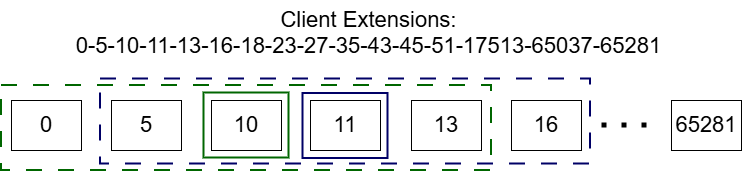
\includegraphics[width=0.8\linewidth]{obrazky-figures/sliding_window.png}
    \caption{Vznik párov $(center, context)$ pomocou kĺzavých okien}
    \label{fig:sliding_window}
\end{figure}

Ako kritérium, ktoré definuje vzdialenosť vektorov sa~použila \textbf{Euklidovská vzdialenosť}\label{emb:euclidean} (tiež známa ako $L_2$ normalizácia). Merchant, Shah a~Castleman vo~svojej publikácii~\cite{euclidean} definujú túto vzdialenosť vzťahom:
\begin{equation}
    d(x_1, x_2) = \sqrt{(X_{21} - X_{11})^2 + (X_{22} - X_{12})^2 + \dots + (X_{2i} - X_{1i})^2}
\end{equation}
kde $x_{2}$ a~$x_{1}$ sú porovnávané vektory. Euklidovská vzdialenosť je teda definovaná ako odmocnina zo~súčtu štvorcov rozdielov jednotlivých súradníc dvoch vektorov.

V spomenutej práci o word2vec~\cite{word2vec} sa~taktiež používa termín \textit{negative sampling} (negatívne vzorkovanie), ktoré je využité aj v~našom prípade. Autori týmto okrem optimalizácie donútili model, aby všetky vektory nemali v~konečnom dôsledku rovnaké hodnoty (toto by vyhovovalo kritériu najmenšej vzdialenosti). Hlavný účel negatívneho vzorkovania je, že~stratová funkcia nebude závisieť len na~vzdialenosti vektorov spadajúcich do~okna stredového vektora, ale aj na~umiestnení v~priestore. Toto sa~dosiahne pridaním náhodných vzoriek do~vyhodnotenia stratovej funkcie, pričom musia byť určitú vzdialenosť ďalej. Konečný predpis stratovej funkcie teda môžeme napísať rovnicou:
\begin{equation}\label{emb:loss_func_word2vec}
    L = \frac{1}{N} \sum_{i=1}^{N} d(v_{c}, v_{p}) + \frac{1}{M} \sum_{j=1}^{M} \max(0, m + d(v_{c}, v_{p}) - d(v_{c}, v_{n,j}))
\end{equation}
\begin{itemize}
    \item $L$ -- Celková hodnota stratovej funkcie (\textit{loss}), ktorú sa~model snaží minimalizovať.
    \item $N$ -- Počet pozitívnych párov.
    \item $M$ -- Počet negatívnych vzoriek pre~každý stredový prvok.
    \item $d(x_1, x_2)$ -- Euklidovská vzdialenosť medzi vektormi.
    \item $v_c, v_p, v_{n,j}$ -- Vektory pre~stredový, pozitívny a~$j$-tý negatívny prvok.
    \item $m$ -- Parameter \textit{margin}, ktorý predstavuje hranicu stability (mieru, o ktorú musí byť ďalej negatívna vzorka ako pozitívna).
\end{itemize}
Na optimalizáciu tohoto word2vec modelu sa~využije Adam optimalizátor, spomenutý v~sekcii~\ref{th:Adam}. Výsledný vektor je normalizovaný, pretože  modely ako word2vec majú tendenciu priraďovať objektom, ktoré sa~v~dátach vyskytujú častejšie, vektory s~väčšou dĺžkou. Cieľom je vyzdvihnúť význam unikátnych príznakov, ktoré sa~nemusia v~dátovej sade vyskytovať až tak často. 

Výsledný optimalizovaný slovník obsahuje kódovanie pre~každú hodnotu parametrov rozšírení, podporovaných skupín a~šifrovacích sád. Následný proces transformácie je vysvetlený nižšie na~príklade pre~konkrétnu hodnotu šifrovacej sady:
\begin{center}
    \texttt{[47, 53, 156, 157, 4865, 4866, 4867, 49171, 49172, 49195, 49196, 49199, 49200, 52392, 52393]}
\end{center}
\begin{enumerate}
    \item \textbf{Vyhľadanie v slovníku:} Každá hodnota je nahradená vektorom z~tabuľky natrénovaného modelu \texttt{word2vec} s dimenziou $d=16$. Príklad pre niektoré konkrétne hodnoty:
    \begin{itemize}
        \item $47 = [4.6517, 2.9216, -7.3098, 5.6010, \dots, 2.9550]$
        \item $53 = [4.1478, 2.7201, -7.3117, 4.9824, \dots, 3.4631]$
        \item $4865 = [0,4449, 0,7706, -6,2535, 0,6406, \dots, 6,6878]$
        \item $4866 = [-1,3111, 0,9946, -5,3234, -1,1976, \dots, 7,3069]$
        \item $49171 = [-4.5830, 1.8724, -2.0464, -5.1714, \dots, 5.6630]$
    \end{itemize}
    Tieto príklady hodnôt sa nachádzajú v~TLS spojeniach najčastejšie. Je možné vidieť, že~blízke hodnoty sú veľmi podobné a~zároveň vzdielné od~hodnôt, s~ktorými sa v~blízkosti často nevyskytujú -- práca pracuje so~zoradenými parametrami, takže väčšinou šif.~sada 47 bude ďalej od~sady 49171. Je~možné vidieť aj~plynulý prechod medzi určitými súradnicami so~zvyšujúcim sa číslom šif.~sady. 

    Niektoré hodnoty šif.~sád sa v~dátovej sade vyskytovali menej, na~ktorých bola často vidieť odchýlka od~spomenutého plynulého prechodu medzi postupnosťou čísel šif. sád. V~ukážke je možné vidieť napríklad menej zastúpenú sadu 159:
    \begin{itemize}
        \item $156 = [3,4118, 2,0199, -7,4019, 3,7070, \dots, 4,6916]$
        \item $157 = [2,1062, 1,8172, -7,2142, 2,0392, \dots, 6,1622]$
        \item $\textbf{159} = [ 6.321, 2.158,  -9.933,  -2.623,\dots, 9.950]$
    \end{itemize}
    
    \item \textbf{Sčítanie vektorov:} Aby sme získali fixný rozmer vstupu pre ľubovoľne dlhý zoznam, vypočítame súčet vektorov:
    \begin{center}
        $\vec{V}_{sum} = [-7.2514, -1.6404, -20.9970, -50.5000, \dots, 28.9763]$
    \end{center}

    \item \textbf{Normalizácia:} Vypočítaný vektorový súčet sa vykoná $L_2$ normalizácia a~pripojí sa k~nemu normalizovaná dĺžka. Pre jednotlivé parametre boli hodnoty pre~normalizáciu dát nastavené analýzou dátovej sady nasledovne: 
    \begin{itemize}
        \item Rozšírenia -- 30.
        \item Śifrovacie sady -- 40.
        \item Podporované skupiny -- 10.
    \end{itemize}

    Výsledný vektor (pre hodnotu normalizovanej dĺžky $l_{norm} = 0.375$) vyzerá pre daný príklad nasledovne:
   $$\vec{V}_{norm} = [-0.0499, -0.0113, -0.1444, -0.3472, \dots, 0.1992, 0.3750]$$
\end{enumerate}

\section{Server Name Indication (SNI)}\label{emb:SNI}
Toto rozšírenie, ako bolo už spomenuté vyššie, je v~textovom formáte. Obsahuje výhradne práve jednu cieľovú DNS adresu servera, s~ktorým má klientská aplikácia nadviazať TLS spojenie~\cite{rfc6066}. Táto DNS adresa sa~skladá z~domén oddelených bodkou, pričom nesmie obsahovať IP adresy a~na konci nesmie byť ukončená bodkou~\cite{rfc1034}.

Existuje mnoho spôsobov ako zakódovať textové dáta na~číselné vektory, ako napríklad aj modelom word2vec spomenutým v~sekcii~\ref{emb:list_embedding}. Tento model sa~tu však nevyužil pre~jeho vlastnosť \textit{vocabulary size} (veľkosť slovníku)~\cite{NLP}. SNI je veľmi variabliná hodnota, kde by bolo nepraktické uchovávať slovník kódovaní, ktorý má fixnú dĺžku ako to~robí word2vec, pretože by mohlo dojsť k~\textit{Out-Of-Words} (OOV) -- nenašlo by sa~kódovanie pre~danú hodnotu v~slovníku. Ďalším kandidátnym prístupom bol model \textit{fast text}. Tento model pridáva k~zakódovaniu rozdelenie slov na~n-gramy, čím odstraňuje problém OOV. To znamená, že~pri tréninku si model ukladá nielen kódovania pre~celé hodnoty (napr. reťazec znakov), ale aj ich častí (\textit{subwords}), a~teda hodnoty približuje morfologicky~\cite{fasttext}. Prvá myšlienka realizácie tohoto prístupu bola importovať už existujúci (ďalej referenčný) model (dostupný na~platforme GitHub~\cite{dns-vsm}). Tento model je však primárne natrénovaný na~doménových menách webových stránok, zatiaľ čo spracovávané dáta obsahovali vysoký podiel špecifických SNI z~aplikačných rozhraní (API). Taktiež bol implementovaný v~staršom rozhraní, ktoré nebolo kompatibilné s~novšou verziou knižnice (\texttt{gensim}~\cite{gensim_migration_guide}). 

Ďalej sa~vyskúšal natrénovať \textit{fast text} model na~dostupnej dátovej sade obsahujúcej prevažne práve API pre~jednotlivé aplikácie. Keďže pre~tento typ modelu nebol počet dát dostatočný (počet v~tab.~\ref{tab:app_connections}), natrénované vektory v~porovnaní s~referenčným natrénovaným modelom na~doménach webstránok ukazovali nízku \textbf{diskriminačnú schopnosť} (odlišnosť rôznych vektorov). To znamená, že~väčšina hodnôt pre~súradnice vektorov sa~nachádzali v~úzkom intervale blízko nuly. Nižšie je uvedené porovnanie pre~SNI \texttt{facebook.com}~\ref{emb:comparision_emb}. Z tohoto dôvodu bol zvolený konečný spôsob kódovania SNI pomocou metódy \textit{hashing trick} (HT).

\begin{lstlisting}[language=Python, caption={Porovnanie hodnôt zakódovaných vektorov pre~SNI \texttt{facebook.com}}, label={emb:comparision_emb}]
# Referencny model (vysoka variabilita/rozptyl)
[ 0.6697, -7.8766,  5.5109, -0.4774,  4.0160, -1.3340,  1.3555, -2.7615, ...]

# Implementovany model (nizka variabilita)
[-0.0779, -0.1497,  0.0155, -0.0263,  0.0231, -0.0253,  0.0154, -0.0785, ...]
\end{lstlisting}

Základom metódy HT je transformácia hondôt do~číselného vektora s~\textbf{fixnou} dĺžkou pomocou hashovania~\cite{scikit}. Algoritmus najskôr rozdelí vstup na~tokeny zadanej dĺžky (môžu sa~vyskytnúť aj kombinácie tokenov), s~ktorými následne pracuje. Algoritmus využíva 2 hashovacie funkcie, pričom obe príjmajú na~vstup práve jednotlivé tokeny a~nie celý dátový vstup. Následný postup je možné opísať v~4 krokoch (vizuálne zobrazené na~schéme \ref{fig:HashingTrick}):~\cite{scikit}

\begin{enumerate}
    \item Token spracuje funkcia $h(x) \rightarrow \{1, ..., n\}$. Táto funkcia vytvorí z tokenu hash, z~ktorého sa získa \textbf{index} (väčšinou operáciou modulo) do~výsledného vektora celého slova. 
    \item Token spracuje funkcia $\xi(x) \rightarrow \{ -1, 1 \}$. Táto funkcia slúži ako ochrana proti kolíziam. Ak je dĺžnka výsledného vektora malá vzhľadom na~veľkosť dátovej sady, je pravdepodobné, že~sa často namapujú dva odlišné tokeny na~rovnaký index funkciou $h(x)$. Náhodným, ale deterministickým priradením znamienka (alternovaním polarity) sa~zabezpečí, že~stredná hodnota chyby spôsobenej kolíziami je nulová, čím sa~predchádza vzniku systematického skreslenia.
    \item Následne sa~na~každý index vo~výslednom vektore, ktorý vznikol z~hashu n-gramu, pripočíta alebo odpočíta hodnota 1 (inkrementácia/dekrementácia) podľa výstupu z~funkcie $\xi(x)$. Ak sa~v~rámci jedného SNI reťazca ten istý index vygeneruje viackrát (či už kvôli opakovaniu n-gramu alebo kolízii), operácia sa~na~danej pozícii zopakuje. Výsledná súradnica vektora je teda daná súčtom všetkých inkrementácií a~dekrementácií prislúchajúcich danému indexu. Napríklad ak~by funkcia $h(x)$ definovala hodnotu 5 pre 3 rôzne tokeny, pričom funkcia $\xi(x)$ by pre~dané tokeny vygenerovala hodnoty $(1,1,-1)$, tak výsledná hodnota vytvoreného vektora na~indexe 5 by bola 1~($1 + 1 - 1$). 
    
    \item Finálnym krokom je normalizácia výsledného vektora. Tento proces zabezpečuje, že~reprezentácia SNI závisí predovšetkým od~relatívneho zastúpenia jednotlivých n-gramov a~ich kontextu, a~nie od~absolútnej dĺžky reťazca.
\end{enumerate}

\begin{figure}[H]
    \centering
    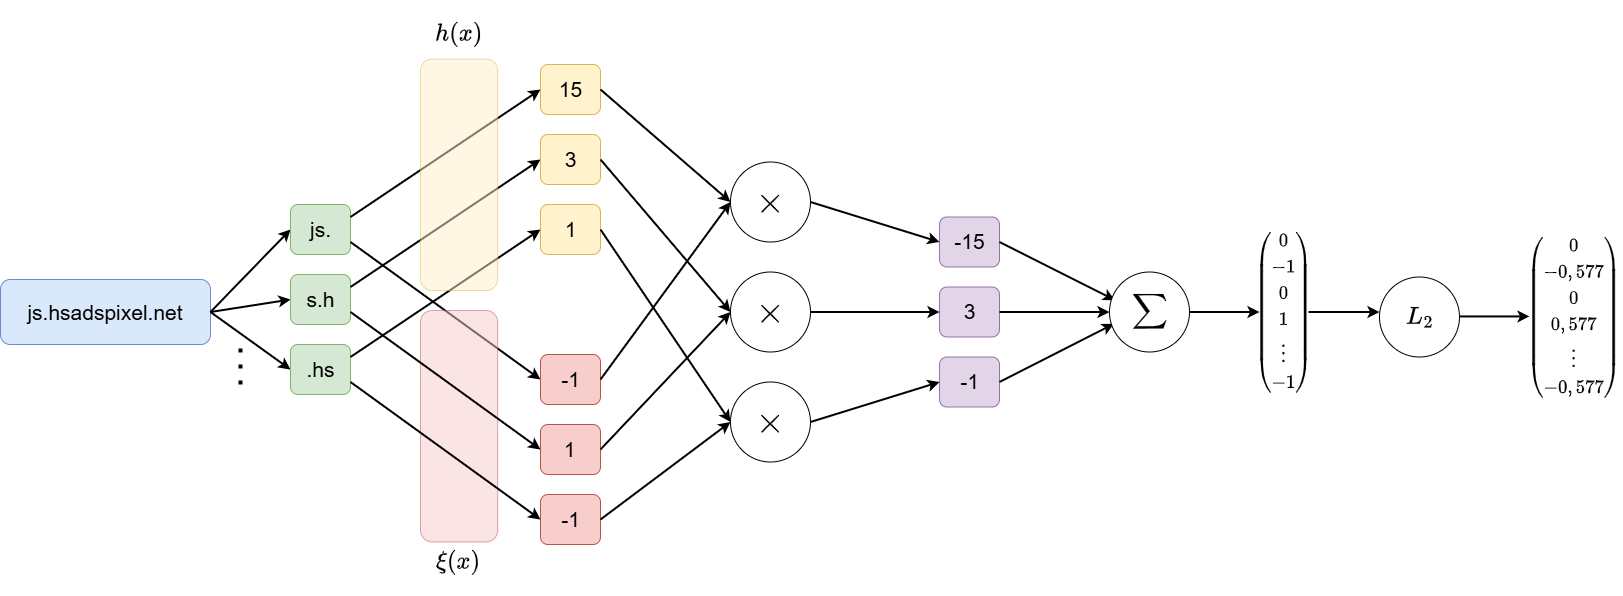
\includegraphics[width=1\linewidth]{obrazky-figures/HashingTrick.png}
    \caption{Kódovanie dát na~16 dimenzionálny vektor pomocou metódy \textit{hashing-trick}}
    \label{fig:HashingTrick}
\end{figure}

Výsledná dĺžka vektora je tzv. hyperparameter, ktorý si volí užívateľ. Je nemenná, pevne daná a~nesúvisí s~dĺžkou tokena. Doporučené hodnoty pre~tento hyperparameter bývajú mocniny čísla~2, práve vďaka zvýšeniu efektivity transformácie hashu funkcie $h(x)$ na~index cieľového vektora pomocou operácie modulo. Tento spôsob implementuje aj knižnica \texttt{Scikit}~\cite{scikit}, ktorú využijeme v~kapitole~\ref{implementation}. V~tejto práci sa určila dĺžka vektora na~16~dimenzií.

\section{Porty}
Ako bolo spomenuté v~sekcii~\ref{emb:portNumbers}, snaha je zakódovať čísla portov tak, aby sme priblížili k~sebe čísla podľa cifier, pričom sa~prioritne zohľadňujú cifry od~najvyššieho rádu po~najnižší. Pre~túto úlohu sa~využil algoritmus predstavený v~práci od~Sivakumara a~Moosaviho~\cite{port_embedding}. Algoritmus spočíva v~rovnici, ktorá definuje deterministickú hodnotu (váhu) pre~každé číslo:
\begin{equation}\label{emb:port_embedding}
    w_i = {\frac{2(N - i + 1) \times 3(N + 1 - i)(N + 2 - i)}{N(N + 1)(N + 2)}}
\end{equation}
\begin{itemize}
    \item $N$: počet cifier v čísle.
    \item $i$: poradové číslo cifry začínajúce od najvýnzamnejšej cifry.
\end{itemize}
Výsledné zakódované čílso portu $p$ môžeme potom zapísať nasledovne:
\begin{equation}
    p = \sum_{i=1}^N{d_i \cdot w_i}
\end{equation}
\begin{itemize}
    \item $d_i$: Cifra čísla portu.
    \item $\omega_i$: Váha pre cifru $d_i$.
\end{itemize}
    
Táto rovnica vytvára rádovo veľký rozdiel medzi jednotlivým ciframi, pričom vyššie cifry dosahujú rozhodujúce hodnoty pre~celé číslo, zatiaľ čo nižšie špecifikujú detaily. Pár príkladov kódovania je možné vidieť nižšie v tabuľke~\ref{tab:port_embedding_examples}:
\begin{table}[H]
    \centering
    \caption{Príklady transformácie a normalizácie hodnôt sieťových portov.}
    \label{tab:port_embedding_examples}
    \begin{tabular}{@{}rr@{}}
        \toprule
        \textbf{Číslo portu} & \textbf{Vypočítaná váha}  \\ \midrule
        420                  & 10.80                     \\
        10000               & 6.86                      \\
        49784               & 54.29                     \\
        65535               & 56.66                     \\ \bottomrule
    \end{tabular}
\end{table}

\section{Výsledný vektor}
Výsledný vektor, ktorý prestavuje už samotný vstup do~autoenkodéru, je tvorený spojením (konkatenáciou) všetkých vybraných parametrov. Pre~vektor bola zvolená dĺžka 182 dimenzií, pričom rozdelenie častí pre~jednotlivé parametre je nasledujúce (vizuálizácia procesu zobrazená na~obrázku~\ref{fig:embedding}):
\begin{figure}[H]
    \centering
    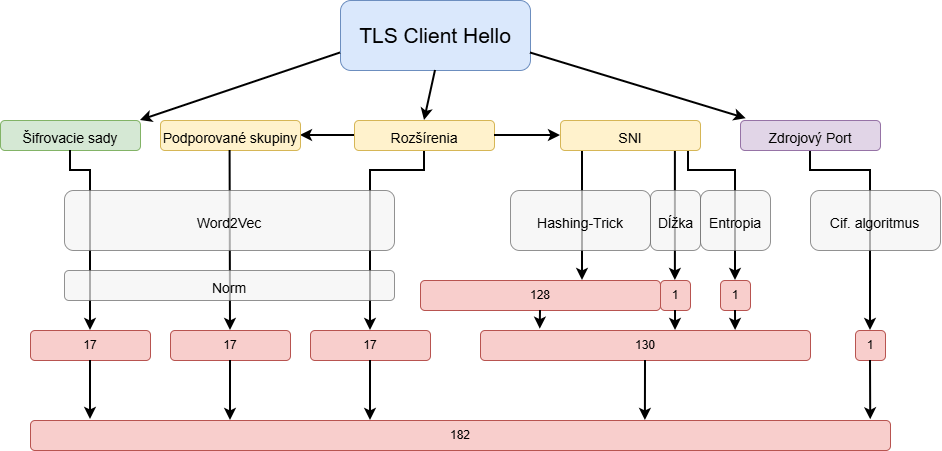
\includegraphics[width=1\linewidth]{obrazky-figures/embedded_vector.png}
    \caption{Proces spracovania dát a~vytváranie vstupného vektora}
    \label{fig:embedding}
\end{figure}
\begin{itemize}
    \item \textbf{SNI}: Tento parameter tvorí najväčšiu časť vektora. Ako bolo už spomenuté v~sekcii \ref{emb:SNI}, určuje DNS adresu servera, z~ktorým chce klientská aplikácia komunikovať, pričom veľakrát táto adresa obsahuje práve názov danej aplikácie. Preto sa~tomuto parametru pridelila dĺžka vo~vektore 128 + 2. 128 dimenzií reprezentuje samotný SNI a~zvyšné 2 dimenzie sú dĺžka SNI, definovaná ako počet znakov, (ktorá bola vynechaná pri~vytváraní kódovania SNI) a~entropia znakov v~názve.  Vybraná bola \textbf{Shannonova entropia}, ktorá bola pridaná z~dôvodu rozlíšenia náhodných domén (typicky malwarové sieťové spojenia) od~domén aplikácií (typicky ľudsky čitateľný názov).

    Táto entropia by mala spĺnať 3 axiómy:
    \begin{itemize}
        \item \textbf{Spojitosť:} Funkcia musí byť spojitá vzhľadom na~pravdepodobnosti $p_i$, čo zabezpečuje stabilitu miery pri~malých zmenách v~rozdelení (v~obore hodnôt funkcie nebudú veľké skoky).
        \item \textbf{Monotónnosť:} Pre~rovnomerne rozdelené javy musí entropia rásť s~počtom možných výsledkov $n$, čo odráža vyššiu neistotu pri~väčšom výbere.
        \item \textbf{Aditivita (Rozkladateľnosť):} Celková neistota musí byť nezávislá od~spôsobu, akým je proces rozhodovania rozdelený na~postupné kroky. To znamená, že~celkové množstvo informácie, ktorú získame, je rovnaké bez ohľadu na~to, či odpoveď na~komplexnú otázku dostaneme naraz, alebo ju vyskladáme postupne cez sériu čiastkových otázok. 
    \end{itemize}
                                               
    Funkcia pre~vyjadrenie entropie sa~dá zapísať nasledovne:
    \begin{equation}
        H(X) = - \sum_{i=1}^{n} P(x_i) \log_2 P(x_i)
    \end{equation}
    $P(x_i)$ reprezentuje pravdepodobnosť, že~sa znak bude v~SNI nachádzať (počet výskytov konkrétneho znaku z~počtu všetkých znakov). To znanmená, že~SNI, ktoré obsahuje veľa znakov, ktoré sa v~ňom opakujú, bude vykazovať nízku hodnotu entropie, práve vďaka nízkej hodnote logaritmu. Naopak, SNI zložené z~veľkého množstva unikátnych znakov bez jasného vzoru bude mať vysokú hodnotu entropie.

    \item \textbf{Rozšírenia, podporované skupiny, šifrovacie sady}: 
    Každému tomuto parametru je pridelených rovnomerne 16 + 1 dimenzií. 16 predstavuje reprezentáciu kódovania pomocou word2vec modelu (sekcia~\ref{emb:word2vec}). 1 dimenzia je vyhradená pre~dĺžku zoznamu daných hodnôt (tieto parametre bývajú v~TLS \textit{Client Hello} zoznamy), pretože pri~tréninku sa~vektor normalizoval. 
    
    \item \textbf{Porty}: Číslam portov bola priradená jedna dimenzia -- práve 1 číslo z~kódovacieho algoritmu. Čísla portov sú typicky vyberané operačným systémom, preto im nebolo pridelené veľké zastúpenie vo~výslednom vektore.
\end{itemize}

\chapter{Návrh štruktúry systému}\label{design}
Ako bolo už spomenuté v~sekcii~\ref{th:autoencoder_types}, existuje mnoho typov autoenkodérov, kde každý má špecifický účel, preto sa~táto kapitola bude venovať práve výberom konkrétneho typu autoenkodéra. Ďalej kapitola predstaví navrhnutý spôsob klasifikácie výstupu (reprezentácie aplikácií). 

\section{Typ modelu}
Cieľom tejto práce je overiť schopnosť autoenkodérov identifikovať konkrétne aplikácie výhradne na~základe parametrov správy \textit{Client Hello}. Vzhľadom na~to, že~sémantický význam a~dôležitosť jednotlivých TLS parametrov pre~neurónové siete tohoto typu nie sú doteraz plne preskúmané, v~experimentálnej časti sa~opierame hlavne o neúplnú (\textit{undercomplete}) architektúru. Táto voľba je motivovaná snahou prinútiť model hľadať skryté súvislosti v~komunikácii bez toho, aby sme ho vopred usmerňovali komplexnejšou modifikáciou dát, čo poskytuje objektívnejší pohľad na~úspešnosť samotnej identifikácie aplikáci.

\textit{Sparse} autoenkodér nebol využitý vzhľadom na~tvar vstupných dát. Samotný vektor pre~SNI je riedky, a~teda pridané vypínanie určitých neurónov zvyšuje riziko straty informácií.

\textit{Denoising} autoenkodér pridáva šum do~vstupných dát, pričom sieť sa~snaží tento šum odstrániť a~zreprodukovať pôvodné čisté vstupné dáta. Hodnoty z~\textit{Client Hello} sú variabilné, kde napríklad rozšírenia mávajú aj pre~rôzne aplikácie podobné hodnoty, ale napríklad hodnoty SNI môžu byť rôzne v~rámci jednej aplikácie. Pridanie šumu by mohlo spôsobiť stratu citlivosti na~\textbf{jemné} rozdiely medzi aplikáciami, ktoré tu považujeme za~rozhodujúci faktor pre~identifikáciu rôznych aplikácií.

Implementácia \textit{variational} autoenkodéra by~bola úspešná, keby sú dáta pre~jednotlivé aplikácie podobné v~zmysle ich štatistického rozdelenia. Keďže však TLS parametre reálnych aplikácií vykazujú vysokú mieru variability, modelovanie množiny dát na~normálne rozdelenie môže byť veľmi nepresné.

\section{Štruktúra modelu}
Autoenkodéry sú teda modely, ktoré rekonštrujú vstup na~čo najpresnejšiu podobu na~výstup, teda sa~ho snažia skopírovať. To znamená, že~systém má obsahovať vstupnú vrstvu a~výstupnú, ktoré majú podľa špecifikácie kódovania dát v~kapitole~\ref{embedding} rovnakú \textbf{fixnú} šírku -- 182 neurónov. Zo vstupnej vrstvy sa~dáta spracovávajú najskôr enkodérom do~latentného priestoru. Veľkosť tohoto priestoru sa~odhadla na~10 až 22 neurónov, pričom experimentálne (kapitola~\ref{experiments}) sa~stanovila konkrétna hodnota. Dekodér následne pomocou vlastných váh prevedie latentný priestor späť na~dimenziu vstupu o veľkosti 182 (samozrejme, s~cieľom zreplikovať hodnoty na~vstupe). Počet skrytých vrstiev bude variabilný, pretože úlohou tejto práce je navrhnúť ideálnu topológiu pre~dosiahnutie vhodnej kapacity modelu. 

Celý model sa~dá popísať ako nelineárne zobrazenie $g \circ f$, kde:
\begin{itemize}
    \item $f$ -- Funkcia enkodéra, definovaná ako: $f: \mathbb{R}^{182} \rightarrow \mathbb{R}^z$, pričom $z \in \langle 10, 22 \rangle $ predstavuje latentný priestor.
    \item $g$ -- Funkcia dekodéra, definovaná ako: $g: \mathbb{R}^z \rightarrow \mathbb{R}^{182}$.
\end{itemize}

Funkcie enkodéra a~dekodéra obsahujú medzi vrstvami aktivačné funkcie. Aj keď najčastejšie používaná aktivačná funkcia je ReLU, v~tejto štruktúre sa~bude používať Tanh. Funkcia ReLU sa~dá zapísať predpisom $f(x) = max(0,x)$ čo znamená, že~funkcia akýkoľvek záporný výsledok vynuluje~\cite{relu}. Toto by mohlo hneď zo~začiatku odstrániť niektoré kritické prvky vstupného vektora, keďže ako je spomenuté v~sekcii~\ref{emb:SNI}, SNI sa~transformuje s~alternujúcou polaritou. Aktivačná funkcia Tanh polaritu zachováva, pričom usmerňuje vstup do~balancovaného intervalu $(-1, 1)$~\cite{tanh}. Matematicky sa~funkcia dá zapísať predpisom:
\begin{equation}
    \text{Tanh}(x) = \frac{e^{x} - e^{-x}}{e^{x} + e^{-x}}
\end{equation}
Výhodou Tanh je jej symetria okolo nuly a~strmší gradient v~okolí počiatku, čo umožňuje citlivejšie reagovať na~jemné rozdiely v~kódovaných dátach. Taktiež Singh vo~svojom webovom článku~\cite{tanh} odporúča Tanh pre~binárnu klasifikáciu dát s~rôznymi polaritami. 

Celú schému systému je možné vidieť na~obrázku~\ref{fig:system_struct}, kde:
\begin{itemize}
    \item $z$: Veľkosť latnentého priestoru (\textit{bottleneck}). 
    \item $n$: Počet funkcií pre~enkodér aj pre~dekodér (majú rovnaký počet transformačných funkcií). Z tohoto vyplýva, že~daný autonekodér obsahuje $2n-1$ skrytých vrstiev (výstupný vektor už skrytý nie je).
    \item $k_i$: Veľkosť redukcie alebo expanzie v~jednom transformačnom kroku. Všeobecne pre~autoenkodéry platí, že~tento krok nemusí byť fixný, ale väčšinou platí, že~dekodér pozostáva z~presne opačných krokov, takže tvorí zrkadlový obraz enkodéra.
\end{itemize}

\begin{figure}[H]
    \centering
    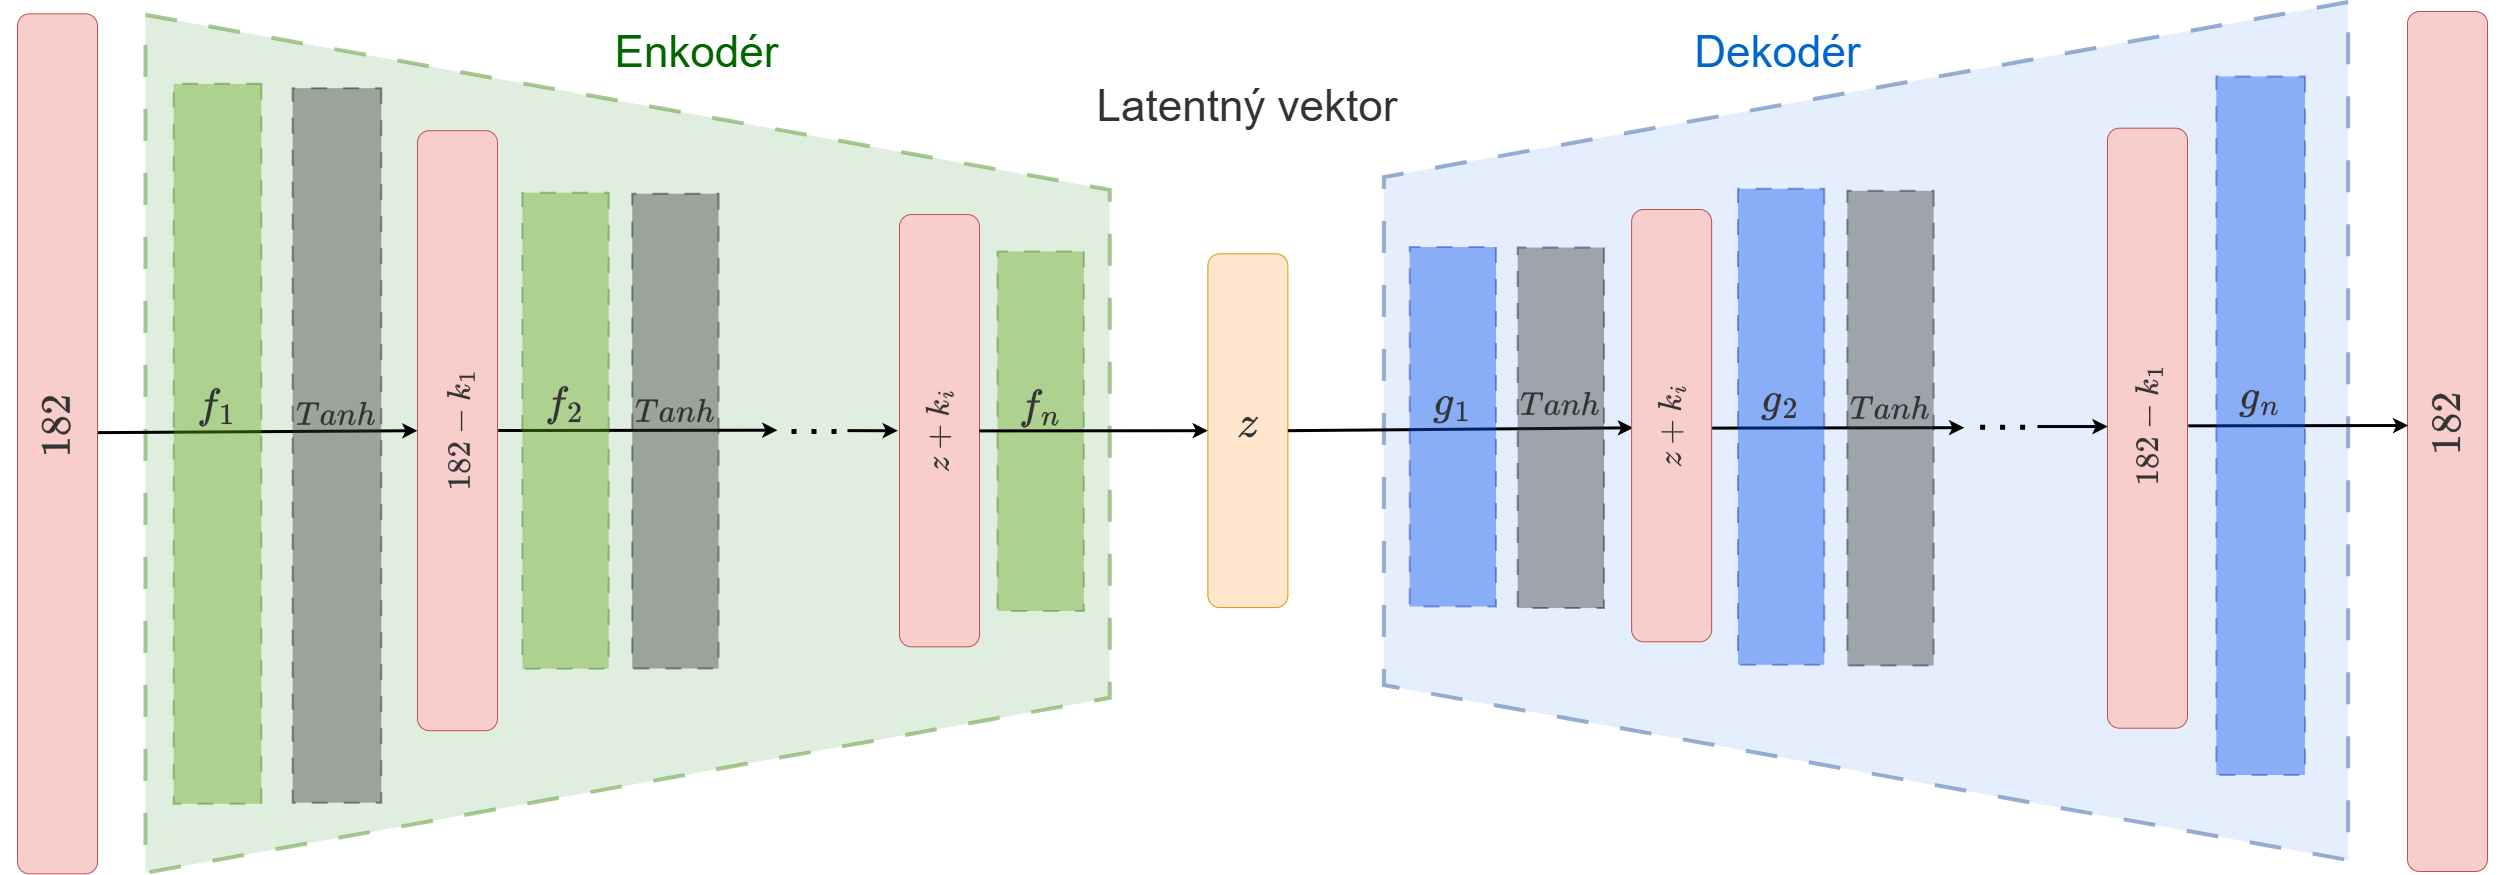
\includegraphics[width=1\linewidth]{obrazky-figures/system_struct.png}
    \caption{Schématické zobrazenie štruktúry systému}
    \label{fig:system_struct}
\end{figure}

\section{Spôsob klasifikácie a~vyhodnocovania}\label{des:classification}
Funkcia autoenkodérov spočíva iba v~rekonštrukcii dát, pričom latentná vrstva slúži hlavne ako prostriedok, ktorý prinúti model vďaka chybe dekodéra upraviť biasy a~váhy v~jednotlivých vrstvách modelu. Výsledná definícia latentného priestoru enkodérovými funkciami vracia úspešnosť učenia až vo~výstupe autoenkodéra, teda zrekonštruovaným vstup. Podobnosť na~vstupný vektor určíme pomocou stratovej funkcie (MSE, sekcia~\ref{th:MSE}), takže identifikácia aplikácií sa~bude vykonávať pomocou \textbf{miery anomality}. 

Kedže autoenkodéry sa~iba učia rekonštruovať dáta, jedná sa~o \textit{unsupervised} (sekcia~\ref{th:unsupervised}) metódu učenia, pretože pre trénovací proces nepotrebujeme mať v~trénovacích dátach \textbf{pridané} označenia (\textit{labely}) požadovaného cieľa. Samotný autoenkodér však nedokáže rozpoznať viacero cieľových aplikácii. Celý klasifikačný systém využije tieto modely k~reprezentícii jednotlivých aplikácií tak, že~jednotlivé aplikácie budú priradené modelom s~najmenšou rekonštrukčnou chybou. Tento proces priradenia dosiahneme natrénovaním modelov systému na~dátach konkrétnej aplikácie. V~tento moment môžme už trénovací proces označiť ako \textit{supervised}. V~prípade reprezentácie cieľovej množiny pomocou jedného modelu sa~jedná o \textbf{binárnu} klasifikáciu, v~prípade využitia viacerých modelov sa~jedná o \textbf{viactriednu} klasifikáciu.

\subsection{Binárna klasifikácia}
Binárna klasifikácia rozdeľuje dáta do~dvoch kategórii: cieľová a~necieľová množina. Modely sa~rozhodujú podľa nejakého medzníka (\textit{threshold}), ktorý bude v~tejto práci predstavovať určitú mieru chyby zo~stratovej funkcie. Na~určenie tejto hodnoty sa~využíva \textbf{0,95 kvantil} distribučnej funkcie strát zaznamenaných počas testovacej fázy na~trénovacích dátach. Tento prístup predpokladá, že~model bude mať úspešnosť na~trénovacích dátach $95\,\%$.

Vyhodnocovanie výsledkov bude prebiehať na~základe tzv. \textit{confusion matrix}, kotrá definuje 4 výsledky z~testovacej vzorky:~\cite{classification}
\begin{itemize}
    \item \textit{True Positive (TP)} -- model \textbf{správne} určil vzorku ako cieľovú aplikáciu.
    \item \textit{False Positive (FP)} -- model \textbf{nesprávne} určil vzorku ako cieľovú aplikáciu.
    \item \textit{True Negative (TN)} -- model \textbf{správne} určil vzorku ako cudziu aplikáciu.
    \item \textit{False Negative (FN)} -- model \textbf{nesprávne} určil vzorku ako cudziu aplikáciu.
\end{itemize}
Maticu je možné vidieť na~schéme~\ref{fig:confusion_matrix}, kde $A$ predstavuje cieľovú a~$\overline{A}$ predstavuje neznámu aplikáciu. 

\begin{figure}[H]
    \centering
    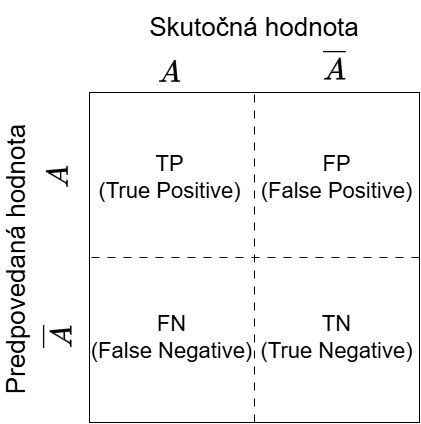
\includegraphics[width=0.4\linewidth]{obrazky-figures/Confusion_matrix.png}
    \caption{\textit{Confusion matrix}}
    \label{fig:confusion_matrix}
\end{figure}

Na vyhodnocovanie úspešnosti a~robustnosti modelov existuje mnoho metrík, pričom najznámejšie sú~\cite{result_statistics}:
\begin{itemize}
    \item \textit{Accuracy}:
    $$ACC = \frac{TN + TP}{FN + FP}$$
    Metrika určuje mieru pravdivých klasifikácií.

    \item \textit{Precision}:
    $$Precision = \frac{TP}{TP + FP}$$
    Metrika určuje pravdepodobnosť, že~ak model určí, že~vzorka je cieľová, tak má~pravdu.

    \item \textit{False positive rate} (FPR):
    $$FPR = \frac{FP}{FP+TN}$$
    Metrika určuje pravdepodobnosť, s~akou model nesprávne klasifikuje cudziu vzorku ako cieľovú~\cite{classification}.

    \item \textit{Recall}:
    $$Recall = \frac{TP}{TP + FN}$$
    Metrika určuje mieru schopnosti modelu správne identifikovať všetky relevantné prípady patriace do~cieľovej množiny (koľko cieľových aplikácií v~testovacej sade model zachytí).

    \item \textit{F1 score}:
    $$F1 = 2 \cdot \frac{Precision \cdot Recall}{Precision + Recall}$$
    Metrika určuje hramonický priemer medzi \textit{recall} a~\textit{precision}. Harmonický znamená, že~hodnota tejto metriky sa~snaží balancovať oba parametry, pričom zabraňuje zlepšeniu jednej na~úkor druhej.
    
    \item \textit{Matthews Correlation Coefficient (MCC)}:\label{des:mcc}
    $$ MCC = \frac{(TP \cdot TN) - (FP \cdot FN)}{\sqrt{(TP + FP)(TP + FN)(TN + FP)(TN + FN)}}$$
    MCC je považovaný za~jednu z~najlepších štatistických metrík pre~binárnu klasifikáciu, pretože ako jedna z~mála berie do~úvahy všetky štyri kvadranty matice zámien (TP, TN, FP, FN) rovnomerne.
\end{itemize}

Aj~keď metrika \textit{Accuracy} pôsobí ako~hlavný rozhodovateĺ o~výkonnosti modelu, nebude vhodná na~tento účeľ, vhľadom na~nevyváženosť dátovej sady. Z~tohto dôvodu sa v~experimentoch sústredíme primárne na~MCC, prípadne na~F1 skóre, ktoré poskytujú objektívnejší pohľad na~výkonnosť modelu~\cite{classification}. Dôležité bude brať ohľad aj na~metriky \textit{Precision}, \textit{Recall} a \textit{FPR} samotné k~identifikácii príčiny zníženej výkonnosti modelu, pretože práve tieto metriky ovplyvňujú hodnotu MCC.

\subsection{Multiclass klasifikácia}\label{des:multiclass}
Základný princíp multiclass klasifikácie je, že~klasifikačný model je schopný nielen rozlíšiť cieľovú vzorku od~cudzej, ale ju aj priradiť ku konkrétnej z~viacerých tried. Existuje viacero spôsobov ako implementovať viactriedne klasifikátory, pričom v~tejto práci sa~využíva \textbf{dekompozícia} na~binárne klasifikácie, ktoré sú popísané v~článku Mohameda Alyho~\cite{multiclass_classification}:
\begin{itemize}
    \item \textit{One-versus-all}\label{des:OVA} (OVA) -- Najjednoduchší spôsob, ktorý redukuje problém klasifikovania medzi $K$ triedami na~$K$ binárnych problémov. To znamená, že~sa vyžaduje $N = K$ klasifikátorov. Keď sa~testuje na~neznámom vzorku, klasifikátor s~najlepšou blízkosťou k~nemu sa~považuje za~víťaza a~vzorok sa~klasifikuje ako trieda, ktorú daný klasifikátor reprezentuje.
    \item \textit{All-versus-all} (AVA) -- Tento prístup redukuje multiclass problém na~$K(K-1)/2$ binárnych klasifikátorov, kde každý model je trénovaný na~rozlíšenie dvojice konkrétnych tried. Porovnávajú sa~tu teda všetky možné dvojice medzi každými triedami. Pri~testovaní neznámej vzorky sa~vzorka predloží všetkým binárnym modelom a~každé rozhodnutie sa~započíta ako hlas pre~danú triedu. Víťazom sa~stáva trieda s~najvyšším počtom získaných hlasov.
    \item \textit{Error-Correcting Output-Coding} (ECOC) -- Tento prístup prideľuje každej triede zo~všetkých $K$ tried ukikátny binárny kód dĺžky $N$, ktorý reprezentuje počet klasifikátorov. Tu musí platiť nerovnosť, aby bolo možné definovať kód pre~každú triedu:
    $$N \geq \log_{2}(K)$$
    Každý z~$N$ klasifikátorov má definovanú binárnu hodnotu $f(x) \in \{0,1\}$, ktorú produkuje na~výstup. Pri~detekcii neznámej vzorky je každému klasifikátoru pridelený vstup, kde výsledný kód vzniká spojením výstupov klasifikátorov. Vzorka sa~pridelí triede, ktorá má kód najmenej vzdialený od~kódu vzorky (napr. pomocou Hammingovej vzdialenosti). Konkrétny príklad je možné vidieť v~tabuľke~\ref{tab:ECOC}. Ak by klasifikátori $f_1$ až $f_7$ vytvorili kód napr. $(0,0,0,0,0,0,1)$, vzorka by sa~klasifikovala ako trieda 1.
    \begin{table}[H]
    \caption{Príklad ECOC klasifikácie}
    \label{tab:ECOC}
    \centering
    \begin{tabular}{|c|c|c|c|c|c|c|c|}
    \hline
            & $f_1$ & $f_2$ & $f_3$ & $f_4$ & $f_5$ & $f_6$ & $f_7$ \\ \hline
    Trieda 1 & 0     & 0     & 0     & 0     & 0     & 0     & 0     \\ \hline
    Trieda 2 & 0     & 1     & 1     & 0     & 0     & 1     & 1     \\ \hline
    Trieda 3 & 0     & 1     & 1     & 1     & 1     & 0     & 0     \\ \hline
    Trieda 4 & 1     & 0     & 1     & 1     & 0     & 1     & 0     \\ \hline
    Trieda 5 & 1     & 1     & 0     & 1     & 0     & 0     & 1     \\ \hline
    \end{tabular}
    \end{table}
\end{itemize}
V našom prístupe využívame OVA, kde každej aplikácii je pridelený model autoenkodéra. Model pre~aplikáciu vzniká konečným trénovaním na~dátach obsahujúcich výhradne TLS spojenia aplikácie. Môže však nastať situácia, že~aplikácia bude mať vysokú rekonštručnú chybu pre~všetky modely (nebude vyhovovať \textit{thresholdu}). V~tomto prípade sa~neklasifikuje aplikácia do~žiadnej cieľovej skupiny, ale ako \textbf{neznáma}.

\chapter{Implementácia klasifikátorov}\label{implementation}
Táto kapitola sa~bude zaoberať už samotnou implementáciou navrhnutého systému v~jazyku \texttt{Python} a~využitých knihovien. Ako prvé kapitola predstaví základnú štruktúru systému pozostávajúcu z~niekoľkých skriptov. Ďalej sa vysvetlí implementácia pre~jednotlivé kódovania vybraných parametrov TLS spojenia. Následne sa~rozoberie spôsob realizácie trénovania modelov a~dynamického vytvárania jednotlivých štruktúr modelov autoenkodérov za~účelom nájdenia optimálnej verzie. 

\section{Základná štruktúra}
Štruktúra implementačnej časti práce vychádza z~postupu riešenia určeného zadaním práce. Prvou časťou bola analýza dát. V~tejto časti sa využívali knižnice \texttt{csv} a \texttt{Pandas}, s~ktorými sa implementovali nasledujúce skripty:
\begin{itemize}
    \item \texttt{dataset\_show.py}: Skript spracováva zdrojovú dátovú sadu do~čitateľnej podoby, čo~sa využilo spočiatku pri analýze dát a~výberu vhodných TLS parametrov. Skript taktiež filtruje dáta podĺa vybraných parametrov. Toto sa využilo pri filtrovaní TLS spojení pre cieľové aplikácie, na~ktorých dátach sa trénovali modely.
    \item \texttt{apps\_show.py}: Skript analyzuje zastúpenie jednotlivých aplikácií v~poskytnutom súbore.
    \item \texttt{join\_docs.py}: Skript spája viacero dokumentov do~jedného na~základe zhody hodnoty v~určenom parametry.
    \item \texttt{shuffle\_csv.py}: Skript náhodne zamieša spojenia v~danom dokumente. Tento skript sa spúšťa.
    \item \texttt{sort\_params.py}: Skript prechádza súbor TLS spojení a~zoraďuje zoznamy číslených hodnôt vybraných TLS parametrov na~kódovanie (rozšírenia, podporované skupiny, šifrovacie sady) pre každé TLS spojenie.
\end{itemize}

Po analýze dát sa implementovala časť kódovania dát. V~tejto časti sa implementovali jednotlivé triedy pre kódovanie každého typu dát (\texttt{PortEmbedder}, \texttt{SNIEmbedder} a~\texttt{EmbeddingViewer}), ktoré sú vysvetlené neskôr. Každá táto trieda poskytuje rozhranie pre zíksanie kódovanie parametru, ktorý reprezentuje. Vytvorenie výsledného zjednoteného vektora z~poskytnutých TLS spojení poskytuje trieda \texttt{ConnectionEmbedder}, ktorá využíva jednotlivé moduly parametrov a~spája ich výsledky pre každé poskytnuté TLS spojenie.

Posledná časť práce sa venovala implementácii modelov a~ich vohodnocovaniu. K~tomuto boli využité triedy \texttt{Undercomplete} a~\texttt{Classifier}. Objekty triedy \texttt{Undercomplete} reprezentujú inštancie autoenkodérov, ktoré sú testované skriptom \texttt{evaluate.py}. Tento skript využíva triedu \texttt{Classifier}, ktorá po~načítaní všetkých požadovaných modelov (uvedených v~konfiguračnom súbore) vykoná klasifikáciu podľa definície v~sekcii~\ref{des:classification}. Celú schému štruktúry systému je možné vidieť v~prílohe~\ref{fig:code_struct}.

\section{Implementácia kódovania TLS parametrov}
Ako bolo uvedené v~kapitole~\ref{embedding}, vybraných bolo 5~parametrov TLS \textit{Client Hello} správy (rozšírnia, podporované skupiny, šifrovacie sady, SNI a~porty), ktoré sa~kódujú rôznymi spôsobmi. Pri~týchto parametroch boli uvedené dve kategórie kódovania:
\begin{itemize}
    \item Učené -- Týmto spôsobom sa~kódujú rozšírnia, podporované skupiny a~šifrovacie sady.  Využíva sa~tu už spomenutý word2vec (sekcia~\ref{emb:word2vec}) model, ktorý sa~učí približovať hodnoty, ktoré sú často v~blízkosti k~sebe. Tento spôsob dynamicky modifikuje sémantiku dát a~pridáva im nelineárne vzťahy, čo môže autoenkodéru priniesť ďalšiu informáciu.
    \item Deterministické -- Týmto spôsobom sa~kódujú čísla portov a~SNI, pričom sa~mení hlavne štruktúra dát. Pre~každé zakódovanie je sémantika dát fixne daná, a~teda~nelineárne vzťahy tu v~tejto podobe ešte neexistujú.
\end{itemize}

\subsection{Učené kódovanie}
Word2vec je model, ktorý (ako bolo už spomenuté v~sekcii~\ref{emb:word2vec}) funguje na~základe optimalizácie vektorov pre~každé slovo v~tréningovej sade. Keďže tento model potrebuje pre~každé slovo záznam v~slovníku vektorov, pri~inicializácii sa~vytvára tabuľka. Vzhľadom na~to, že~môžu existovať rozdiely v~testovacej a~trénovacej sade, pri~testovaní model môže naraziť na~hodnotu, ktorú pri~tréningu nevidel, a~teda je potrebné aby všetky možné hodnoty boli v~tabuľke definované. Preto sa~pred~trénovaním pridajú nielen hodnoty obsiahnuté v~trénovacích dátach, ale aj hodnoty, ktoré sú \textbf{definované} v~registroch IANA~\cite{iana_tls_parameters, iana_tls_extensions}. Toto zabezpečuje modul \texttt{TableCreator}, ktorý je možné spustiť skriptom \texttt{Table\_creator.py}. Výsledná tabuľka je uložená pomocou knižnice \texttt{PyTorch} ako vyhľadávacia tabuľka implementovaná triedou \texttt{nn.Embedding}. Táto vrstva obsahuje viacrozmerné pole váh typu \textbf{\texttt{torch.Tensor}} (ďalej tenzor) a~pri použití vracia zodpovedajúce kódované vektory.

Akonáhle sa vytvorí tabuľka s~náhodnými hodnotami, pomocou modulu \textit{SkipGramTrainer} model prechádza na~proces tréningu. Po načítaní tabuliek sa~vytvoria z~trénovacých dát zo~vstupu páry pre~kĺzavé okno. Tieto páry sa trénujú pomocou \textit{triplet loss} funkcie, ktorá roprezentuje návrh negatívneho vzorkovania v~sekcii~\ref{emb:word2vec}. Ako optimalizátor sa~používa Adam (sekcia ~\ref{th:Adam}) z~knižnice \texttt{torch.optim}. Následne sa~vypočíta vzdialenosť od~pozitívnych vektorov a~negatívnych vektorov (od ktorých sa~model snaží stredový vektor vzdialiť) pomocou euklidovej vzdialenosti (sekcia~\ref{emb:euclidean}) s~tým, že~počet negatívnych vektorov je 10. Tento proces sa~v~jednej epoche (iterácii) vykoná niekoľkokrát, pretože sa~využíva učenie po~dávkach (\textit{batches}). To znamená, že~sa tabuľka neoptimalizuje až po~vypočítaní chyby pre~všetky trénovacie vzorky, ale hneď po~určitom počte vzoriek (dávke), konkrétne 64 vzoriek. Stratová funkcia pre~optimalizáciu sa~implementovala podľa rovnice~\ref{emb:loss_func_word2vec}.

\subsection{Deterministické}
Pri kódovaní čísel portov sa~využíva algoritmus definovaný v~kapitole~\ref{emb:port_embedding}, ktorý implementuje trieda \texttt{PortEmbedder}. Tento algoritmus bol však príliš zhovievavý vzhľadom na~váhu nižších cifier, čo zapríčinilo že~niektoré čísla portov s~väčšou hodnotou mali v~konečnom súčte cifier menšiu celkovú hodnotu ako čísla menšie (viz. tabuľka~\ref{tab:port_comparison}). Preto je v~implementácii algoritmus upravený na~nasledujúci vzorec pre~váhu každej cifri čísla portu:
\begin{equation}
    w_i = \frac{2^{N - i} \cdot 3^{(N + 1 - i)(N + 2 - i)^{v}}}{N(N + 1)(N + 2)}
\end{equation}
Výsledné kódovanie $p$ sa vypočíta rovnako ako v~pôvodnom algoritme:
\begin{equation}
    p = \sum_{i=1}^N{d_i \cdot \omega_i}
\end{equation}
Tento vzorec zväčšuje vplyv vyššej cifry exponenciálne, čo zabraňuje prekrývaniu významu jednotlivých rádov a~zabezpečuje, že~zmena na~vyššej pozícii čísla portu má vždy dominantnejší dopad na~výslednú hodnotu než \textbf{akékoľvek} zmeny na~nižších pozíciách. Výsledná hodnota sa~následne \textbf{normalizuje} hondotou pre~port 65535, čo zabezpečí rozsah v~intervale $(0,1)$. Premenná $v$ vo~vzorci predstavuje istý váhový faktor pre~vzorec, ktorým sa~reguluje vplyv nižšej cifry, keďže bez nej algoritmus úplne potlačil vplyv nižších cifier. Čím nižsiu má hodnotu, tým menší je rozdiel medzi kódovaním na~nižších a~vyšších pozíciach.

SNI sa~kóduje technikou \textit{hashing-trick} (HT) (sekcia~\ref{emb:SNI}), ktorú implementuje trieda \texttt{SNIEmbedder}. Tu sa~využíva trieda \texttt{HashingVectorizer} z~knižnice \texttt{scikit-learn}~\cite{scikit}. Objekt tejto triedy vykoná HT s~dĺžkou n-gramov rovnej 3 a~zredukuje celé slovo do~normalizovaného vektora s~veľkosťou 128. Tento vektor je typu \texttt{numpy.array} z~knižnice \texttt{NumPy}, ktoré sa~následne prekonvertuje na~pole typu tenzor z~knižnice \texttt{PyTorch}. Následne sa~vypočíta entropia pre~dané slovo, ktorá je implementovaná ako Shannonova-entropia~\cite{ShannonEntropy}. 

Celý vektor pre~SNI vzniká spojením HT kódovania, čísla entropie pre~dané SNI a~jeho dĺžkou. Tento vektor je uložený do~poľa tenzor.

\subsection{Výsledný vektor}
Výsledný vektor vzniká ako konkatenácia všetkých kódovaní v~nasledujúcom poradí: SNI, zdorjový port klientskej aplikácie, klientská šifrovacia sada, rozšírenia a~podporované skupiny. Tento proces vytvára inštancia triedy \texttt{ConnectionEmbedder}, ktorá postupne prechádza parametre pripojenia a~jednotlivo ich kóduje a~ukladá do~poľa typu tenzor.

\section{Implementácia modelu}
Pred spúšťaním skriptov pre~interakciu a~vytváranie modelov sa~v~zložke nachádza súbor \texttt{config.json}, v~ktorom sa~nastavujú rôzne parametre, ako napríklad požadovaná štruktúra modelu, názov modela, s~ktorým sa~aktuálne pracuje, rýchlosť učenia\dots Pre~implementáciu modelu bola využitá hlavne knižnica \texttt{PyTorch}. Model príjma na~vstup zakódované dáta, a~teda pred~tréninkom sa~celá trénovacia a~testovacia sada zakóduje pomocou skriptu \texttt{make\_test\_data.py}, ktorý vytvorí tabuľku kódovaní pre~model. Model je implementovaný v~triede \texttt{Undercomplete}, ktorá dedí z~triedy \texttt{nn.Module}~\cite{nn.module}. Táto rodičovská trieda z~knižnice \texttt{PyTorch} poskytuje základné rozhranie/triedu pre~neurónové siete. Po vytvorení a~natrénovaní sa~model ukladá do~súboru typu \texttt{PyTorch model file}, kde sa~ukladajú nielen optimalizované váhy a~biasy, ale celá štruktúra (konkrétne objekt) modelu. V~prípade tejto práce sa~využívajú aj ďalšie triedy, ktoré z~\texttt{nn.Module} dedia:
\begin{itemize}
    \item \texttt{nn.Sequential} -- Tento modul slúži ako kontajner, ktorý spája moduly tak, že~výstup z~funkcie ihneď presmeruje na~vstup do~nasledujúcej~\cite{pytorch.sequential}. V~tejto práci sa~využíva na~spájanie jednotlivých vrstiev enkodéra a~dekodéra, teda celkový model obsahuje 2 takéto podmodely.  
    \item \texttt{nn.Linear} -- Predstavuje plne prepojenú vrstvu neurónovej siete, ktorá vykonáva lineárnu transformáciu vstupu podľa vzorca $y = x A^T + b$~\cite{pytorch.linear}. Matica $A$ tu predstavuje vrstvu neurónov, kde jeden riadok matice reprezentuje váhy pre~jeden neurón. Vektor $b$ reprezentuje vektor biasov, kde jedna hodnota patrí práve jednému neurónu. Práve tieto parametre sú reprezentované ako \textit{Variables} (neskôr v~sekcii~\ref{imp:forward_pass}).
\end{itemize}

Model sa~zostavuje dynamicky podľa štruktúry uvedenej v~\texttt{congfig.json}. Najskôr sa~zostaví \texttt{nn.Sequential} funkcia pre~enkodér, do~ktorej sa~podľa dimenzií a~počtu vrstiev modelu vložia dvojice \texttt{nn.Linear} s~\texttt{nn.Tanh}. Takto sa~postupne prepojí selá topológia, pričom posledná funkcia enkodéru bude \texttt{nn.Linear}. Vytvorenie dekodérovej funkcie prebieha zrkadlovo opačne, pričom sa~začína od~latentnej dimenzie a~pokračuje až do~dimenzie vstupu. Celkovo teda správanie modelu vieme definovať jednou zloženou funkciou (nazývanou \texttt{forward()}) definovanou:
\begin{lstlisting}[language=Python, caption={Hlavná funkcia autoenkodéru}]
def forward(self, input):
    encoded = self.encoder(input)
    decoded = self.decoder(encoded)
    return decoded
\end{lstlisting}

Akonáhle sa~vstupný tenzor spracuje, na~výstupný tenzor sa~zavolá funkcia \texttt{backward()}, ktorá nastaví gradienty pre~všetky premenné (parametre), ktoré sa~podieľali na~výpočte a~majú nastavenú vlastnosť \texttt{requires\_grad=True} (viz. obrázok~\ref{fig:LR_Gradient}). Gradienty sú po výpočte uložené v atribúte \texttt{.grad} každého objektu premennej, ktorý reprezentuje váhy alebo biasy modelu.

\subsection{Dopredný prechod (\textit{forward pass})}\label{imp:forward_pass}
Trieda \texttt{nn.Module} umožňuje definovať metódu \texttt{forward()}, ktorou sa~špecifikuje správanie modelu pri~spracovaní vstupných dát. Metóda je špeciálna v~tom, že~v~prostredí triedy \texttt{nn.Module} si model sleduje všetky operácie vykonané so vstupnými tenzormi, ktoré následne využíva metóda \textbf{AutoGrad} opísaná v~dokumentácii knižnice \texttt{PyTorch}~\cite{AutoGrad, pytorch.autograd}.

Knižnica tu využíva tzv. \textbf{výpočtový graf} (\textit{Directed Acyclic Graph} -- DAG), potrebný na~spätný výpočet gradientov pri~\textit{backpropagation} (sekcia~\ref{th:backpropagation}), ktorý je tvorený:
\begin{itemize}
    \item \textbf{Uzlami}: Predstavujú objekty typu \texttt{torch.autograd.Function}, teda definíciu funkcie neurónu.  kde vytvára z~gradientov na~výstupe gradient pre~vstup.
    \item \textbf{Hranami}: Reprezentujú tok dát (smer od~vstupu do~výstupu).
    \item \textbf{Premennými} (\textit{Variables}): Premenlivé objekty, ktoré definujú výsledky funkcií počas \textit{forward pass}, pričom si uchovávajú aj históriu výpočtu (ktorý neurón ich vypočítal). Tieto objekty obsahujú teda nasledovné parametre:~\cite{pytorch.autograd, pytorch.leaf_vs_nonleaf}

    \begin{itemize}
    \item \texttt{data}: Reprezentuje samotné tenzorové úložisko s~numerickými hodnotami.
    \item \texttt{grad}: Pole určené na~ukladanie gradientov vypočítaných počas spätnej propagácie.
    \item \texttt{grad\_fn}: Ukazovateľ na~objekt \texttt{Function} (uzol grafu), ktorý premennú vygeneroval. Pri~vstupných (\textit{leaf}) premenných má hodnotu \texttt{None}.
    \item \texttt{is\_leaf}: Logický príznak, ktorý odlišuje vstupné parametre od~medzivýsledkov výpočtového grafu.
    \item \texttt{requires\_grad}: Príznak riadiaci mechanizmus automatickej diferenciácie. Ak je \texttt{True}, operácie s~touto premennou sa~zaznamenávajú do~dynamického grafu.
    \end{itemize}
    
\end{itemize}
Tento graf sa~vytvára tzv. \textit{define-by-run execution}, čo znamená, že~uzol je vytvorený v~momente, keď sa~prechádza neurónom siete (počas \textit{forward pass} -- vykonávanie funkcie neurónu). Tento spôsob vytvárania nedefinuje predom štruktúru grafu. 

\subsection{Spätný chod (\textit{backward pass})}\label{imp:backward_pass}
Akonáhle sa~vstupný tenzor spracuje, na~výstupný tenzor sa~zavolá funkcia \texttt{backward()}. Táto funkcia spôsobí, že~\texttt{PyTorch} začne prechádzať graf výpočtu od~posledného uzla, pričom postupne pomocou reťazového pravidla (sekcia~\ref{th:backpropagation}) počíta gradienty uzlov typu \texttt{Variable} (konkrétne dátový typ tenzor). Ako je spomenuté vyššie, tieto objekty obsahujú parameter \texttt{is\_leaf}, čo indikuje, či sa~jedná o tzv. \texttt{\textbf{leaf node}}. \texttt{PyTorch} sa~snaží byť totiž efektívny pri~využívaní pamäte, a~keďže výpočty prebiehajú na~GPU, ukladá iba tie gradienty, ktoré sú vypočítané pre~\texttt{leaf} uzly a~obsahujú $requires\_grad=True$~\cite{AutoGrad, pytorch.autograd}. \texttt{Non-leaf} uzly slúžia iba ako medzikrok a~po ich využití v~tomto procese sa~ich vypočítané gradienty uvoľnujú z~pamäte. Inak povedané, \texttt{leaf} uzly sú uzly, ktoré nevznikli výpočtom, ale sú pevne dané a~slúžia ako vstupujúce hodnoty do~grafu. 

Nižšie na~obrázku~\ref{fig:AutoGrad} je možné vidieť ukážku vzniku gradientov pre~jeden neurón (celkovo vrstvu) s~dimenziou vstupu~3. Dopredný prechod ukazujú biele šípky, pričom sa vypočítavajú hodnoty pre~jednotlivé premenné grafu. Každá premenná má~nastavené \texttt{requires\_grad} na~hodnotu True (okrem vstupov), aby ich optimalizátor mohol ovplyvniť. Všetky premenné obsahujú taktiež atribút \texttt{.grad}, kde sa~ukladá vypočítaná hodnota gradientu pri \textit{backpropagation}. Nelistové premenné majú uvedený aj~atribút \texttt{grad\_fn}, ktorý referuje na funkciu pomocou ktorej boli vytvorené. Samotný neurón je reprezentovaný fialovým rámom, ktorý obsahuje váhy pre každý vstup a~jednotný bias. Po~spracovaní výstupu stratovou funkciou sa zavolá funkcia \texttt{backward()}, ktorá inicializuje proces \texttt{backpropagation}. Tento proces postupne od~konca dopredného chodu (od~stratovej funkcie s~počiatočnou hodnotou gradientu~1) vypočítava reťazovo gradienty (červená šípka) pre~jednotlivé premenné s~využitím derivácie funkcie, ktorá ich vytvorila (\texttt{grad\_fn}) a~hodnoty gradientu predchádzajúcej z~predchádzajúceho uzla. Vypočítané hodnoty sa uložia do~\texttt{.grad} parametru premennej (zelená šípka). Tento proces iteruje dokiaľ nemajú váhy a~biasy neurónu/vrstvy definované gradienty pre~optimalizátor.  
\begin{figure}[H]
    \centering
    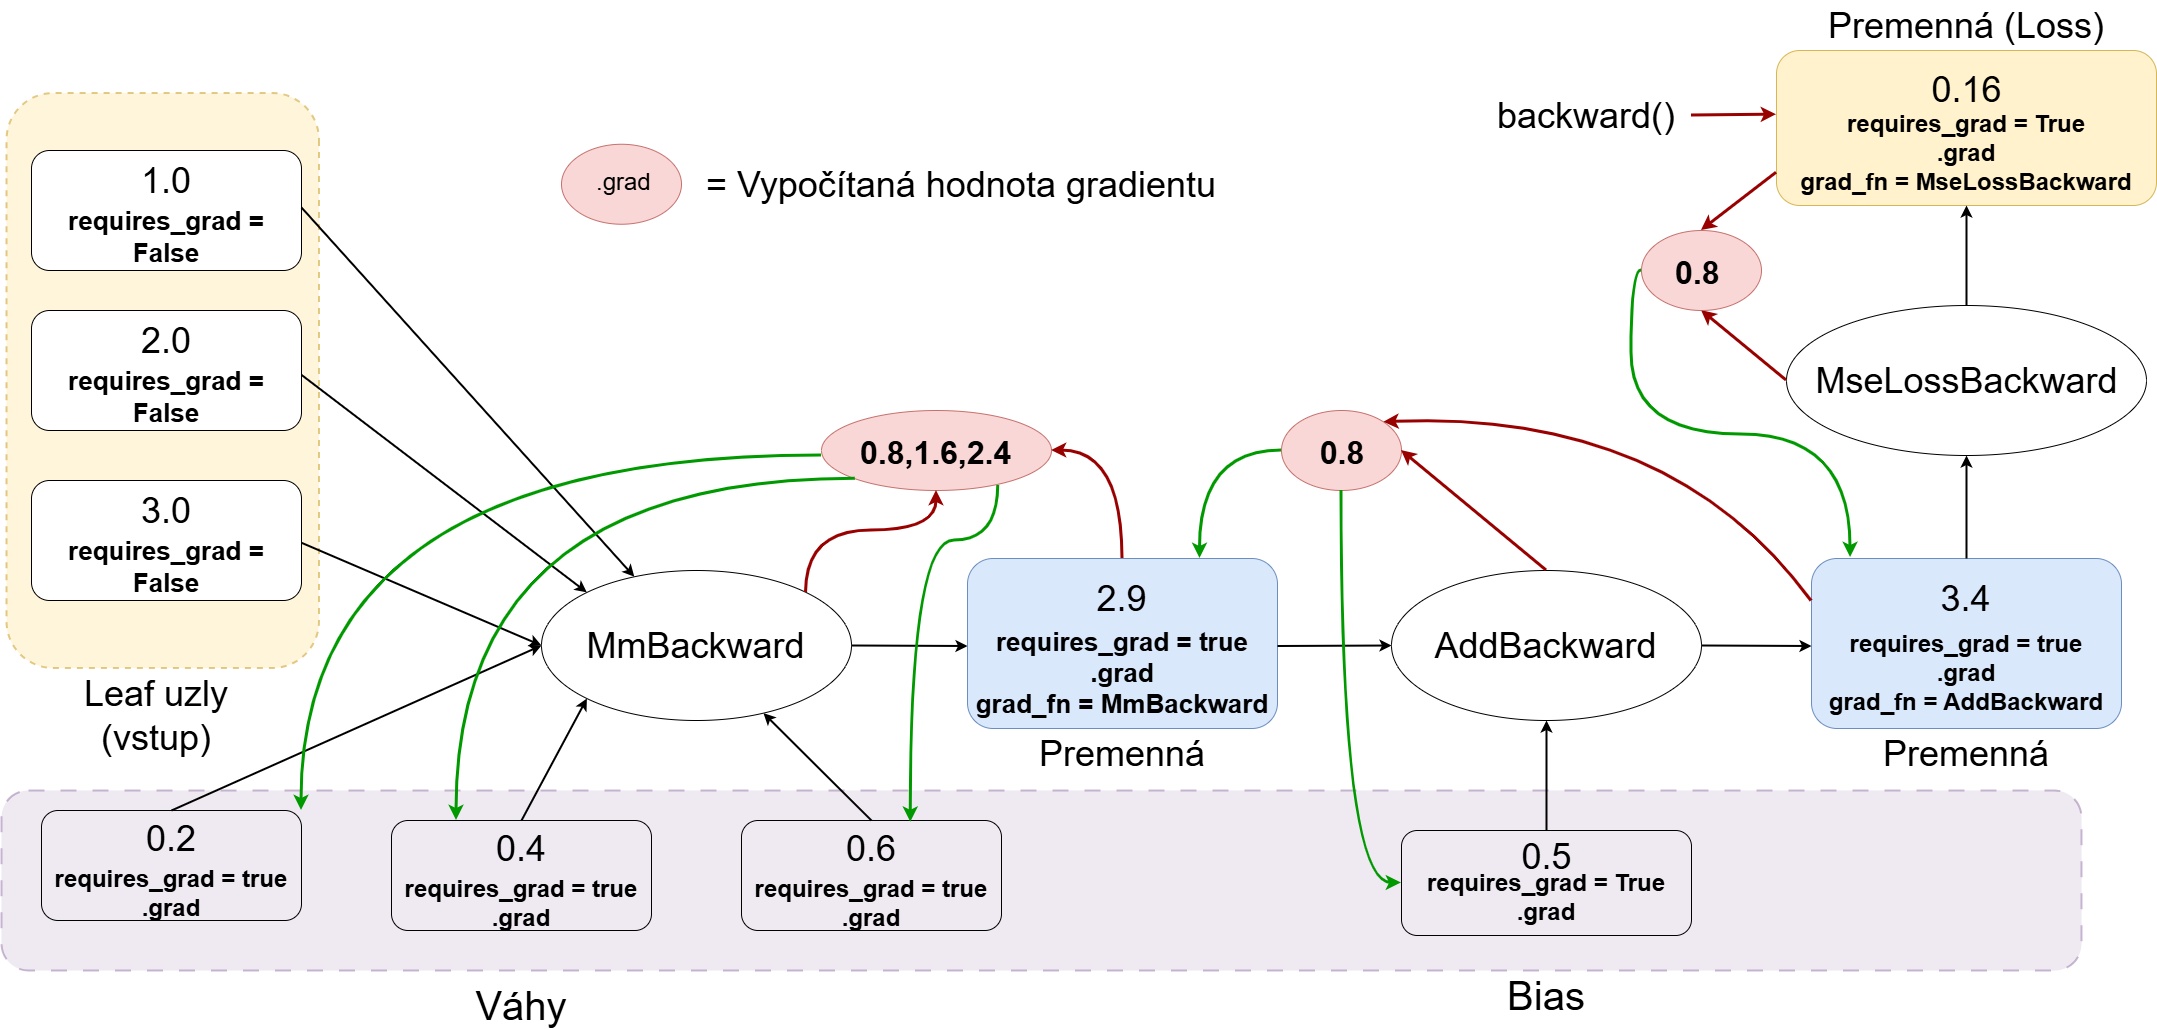
\includegraphics[width=1\linewidth]{obrazky-figures/GradientPyTorch.png}
    \caption{Ukážka vzniku gradientov pre~jeden neurón/vrstvu.}
    \label{fig:AutoGrad}
\end{figure}

\subsection{Optimalizácia}\label{imp:optimalisation}
Na optimalizáciu sa~využíva optimalizátor Adam (sekcia~\ref{th:Adam}) implementovaný knižnicou \texttt{torch.optim}~\cite{pytorch.optim}, ktorý je reprezentovaný objektom \texttt{torch.optim.Adam}. Do tohoto objektu sa~pri~inicializácii vkladajú tenzori modelu, ktoré má sledovať a~optimalizovať, a~\texttt{learning rate} (miera učenia). Ďalej všetky optimalizátory tejto knižnice ako aj Adam implementujú metódu \texttt{optim()}, ktorá definuje metóda samotného optmializačného procesu na~základe typu optimalizátora. Táto metóda sa~volá hneď po~metóde \texttt{backward()}.

\subsection{Proces trénovania modelu}
Keďže model dedí z~triedy \texttt{nn.Module}, pred~zaznamenávaním priechodu vstupných dát sieťou je potrebné nastaviť model do~trénovacieho režimu metódou \texttt{train()}. Keďže \texttt{PyTorch} nevymazáva výsledné gradienty v~listových uzloch, je potrebné pred~každou epochou vynulovať vypočítané gradienty metódou optimalizátora \texttt{zero\_grad()}. Následne trénovací proces prebieha v~niekoľkých epochách, pričom jedna epocha sa~skladá zo~všetkých činností popísaných v~sekciach~\ref{imp:forward_pass},~\ref{imp:backward_pass},~\ref{imp:optimalisation}.

Počas trénovania sa~využíva metóda \textit{\textbf{early stopping}}\label{early_stopping}, ktorá slúži na~predčasné zastavovanie tréningu, pokiaľ sa~model už pri~učení nezlepšuje o nejakú minimálnu odchýlku. Pre~toto sa~využíva knižnica \texttt{Ignite}, ktorá poskytuje triedy \texttt{Engine} a~\texttt{EarlyStopping}:
\begin{itemize}
    \item \texttt{Engine} -- Táto trieda predstavuje jadro knižnice a~slúži ako abstrakcia trénovacej slučky, ktorá opakovane spúšťa používateľom definovanú funkciu (v~našom prípade to~bude celá činnosť jednej epochy). Riadi sa~systémom udalostí (\textit{Events}), ktoré umožňujú spúšťať špecifické akcie v~rôznych momentoch trénovania (napr. na~začiatku iterácie, po~skončení epochy alebo pri~ukončení celého procesu). V~každom kroku engine aktualizuje svoj vnútorný stav (\texttt{State}), v~ktorom uchováva aktuálne metriky a~parametre behu~\cite{pytorch.ignite_engine}.
    \item \texttt{EarlyStooping handler} -- Táto trieda implementuje logiku pre~\textit{early stopping}. Pred spustením objektu \texttt{Engine} sa~mu pridá tento handler, s~požadovanými parametrami ako je trpezlivosť, skórovacia funkcia pre~porovnanie a~minimálna odchýlka.
    Handler po~každej epoche zavolá \texttt{score\_function} a~ak sa~toto skóre nezlepší o viac ako \texttt{min\_delta} počas stanoveného počtu po~sebe idúcich epoch (tento počet definuje trpezlivosť), \texttt{EarlyStopping} automaticky nastaví príznak pre~ukončenie behu \texttt{Engine}~\cite{pytorch.ignite_handlers}.
\end{itemize}

Na konci tréninku sa~ukladá prah chyby (\textit{threshold}), ktorý je dostupný taktiež v~súbore \texttt{thresholds.json}, kde je možné ho pre~daný model modifikovať. Tento prah sa~vytvára po~tréningu ako 0.95 percentil pre~sadu poskytnutých trénovacích dát.

\subsection{Klasifikácia}\label{imp:classification}
Klasifikácia prebieha pomocou triedy \texttt{Classifier}. Táto trieda využíva modely zo~súboru \texttt{config.json}, pričom každému spracovanému spojeniu priradzuje najbližší model, teda model s~najmenšou rekonštručnou chybou. 

V prípade binárnej klasifikácie je potrebné zapísať mená súborov využitých modelov do~\texttt{config.json}, konkrétne do~parametru \texttt{test\_models\_name}, a~k nim príslušné aplikácie v~tvare: \texttt{''Model.pth'':} \texttt{''DestAppName''}. Taktiež do~parametru \texttt{dest\_app\_name} je potrebné uviesť \textbf{hľadanú} aplikáciu, pretože klasifikácia považuje za~cieľové aplikácie iba tie, ktoré sú uvedené v~tomto parametry. Trieda v~tomto režime pridelí spojeniu daný model, ak rekonštrukčná chyba neprekračuje prah definovaný pre~uvedený model.

V prípade viactriednej klasifikácie je potrebné do~parametru \texttt{test\_models\_name} uviesť všetky dvojice (meno testovaného modelu: hľadaná aplikácia) a~všetky hľadané aplikácie do~parametru \texttt{dest\_app\_name}. V~tomto režime trieda \texttt{Classifier} implementuje systém OVA (sekcia~\ref{des:OVA}). Každému spojeniu je pridelených niekoľko kandidátnych modelov, pre~ktoré má rekonštrukčná chyba dostatočne nízku hodnotu. Ak existujú kandidátne modely, za~reprezentujúceho pre~aplikáciu sa~vyberie model s~najnižšou chybou. Ak kandidátne modely neexistujú, aplikácia sa~považuje sa~neznámu.

Pre vyhodnotenie výsledkov slúži skript \texttt{evaluate.py}. Tento skript vytvára objekt \texttt{Classifier}, pomocou ktorej vyhodnocuje, či správny model správne vyhodnotil svoju aplikáciu za~cieľovú. Definícia systému, kedy model považuje predikciu aplikácie za~úspešnú je uvedená nižšie v~tabuľke~\ref{tab:decision_logic}. Špecifický prípad je situácia, keď je aplikácia neznáma a~je priradená modelu, ktorý hľadá \textbf{necieľovú} (neznámu) aplikáciu. Tento prípad sa~považuje za~TN, pretože sa~testuje systém s~danými autoenkodérmi ako \textbf{celok}, ktorý správne detegoval aplikáciu za~neznámu.

\begin{table}[H]
\centering
\caption{Rozhodovacia logika klasifikácie a~priradenie k~matici zámien}
\label{tab:decision_logic}
\begin{tabularx}{\textwidth}{l l c X}
\toprule
\textbf{Skutočnosť} & \textbf{Predikcia systému} & \textbf{Výsledok} & \textbf{Odôvodnenie} \\ \midrule
Hľadaná & Správny model & \textbf{TP} & Úplná zhoda medzi skutočnou aplikáciou a~jej modelom. \\ \addlinespace
Hľadaná & Iný model / Žiadny model & \textbf{FN} & Systém hľadanú aplikáciu neidentifikoval alebo priradil nesprávne. \\ \addlinespace
Cudzia & Model hľadanej aplikácie & \textbf{FP} & Falošné označenie cudzej prevádzky za~hľadanú aplikáciu. \\
Cudzia & Model cudzej aplikácie / Žiadny & \textbf{TN} & Správne ignorovanie prevádzky, ktorá nie je predmetom záujmu. \\ \bottomrule
\end{tabularx}
\end{table}

Podľa súboru s~konfiguračnými paramterami \texttt{config.json} je možné natrénovať aj niekoľko variant modelov sekvenčne spustením skriptu \texttt{train\_model\_variants}, ktorý natrénuje modely jedným z~dvoch spôsobov, ktoré udáva parameter \texttt{proportional\_scaling} (PS):
\begin{itemize}
    \item Proporcionálne (PS = \texttt{True}):\label{imp:proportional} Vrstvy enkodéra pre~jednotlivé modely sa~vytvárajú postupne od~najväčšej po~najmenšiu s~tým, že~medzi každou vrstvou je veľkostne rovnaký rozdiel v~počte neurónov. Používateĺ tu zadáva iba počet vrstiev do~parametra \texttt{max\_layers}, krok medzi vrstvami sa~vypočíta na~základe uvedenej štruktúry. Takto sa~vytvorí niekoľko modelov, pričom počet vrstiev od~vstupnej (vrátane) po~latentnú sa~inkrementuje až do~hodnoty uvedenej v~parametri \texttt{max\_layers}. Šírka jednotlivých vrstiev je teda premenlivá a~závisí od~celkového počtu vrstiev modelu a~veľkosťou latentného priestoru (veľkosť vstupnej vrstvy je fixná). Príklad vytvorenia proporcionálneho modelu s~5 vrstvami a~latentným priestorom veľkosti 14 je pri~fixnom vstupe 182 vypočítaný krok $\Delta d = 42$, čím vzniká symetrická architektúra enkodéra s~rozložením neurónov:
    $$182 \xrightarrow{-42} 140 \xrightarrow{-42} 98 \xrightarrow{-42} 56 \xrightarrow{-42} 14$$
    \item Lineárne (PS = \texttt{False}):
    V~parametri \texttt{mid\_layers\_to\_test} sa staticky definujú vrstvy enkodéra, do~ktorého používateľ zadáva cieľovú postupnosť dimenzií (napr. \texttt{[182, 128, 96, 20]}). Skript následne nevygeneruje iba jeden model, ale sériu modelov, kde v~každom kroku pridá jednu ďalšiu vrstvu zo~zadanej postupnosti, pričom platí postupnosť vrstiev od~najväčšej po~najmenšiu (182-20, 182-128-20, 182-128-96-20 podľa uvedeného príkladu). Tento spôsob sa~vykoná, ak je parameter \texttt{combine\_dimensions} nastavený na~\texttt{False}.
    
    \item Kombinovane (PS = \texttt{False}): Tento režim vygeneruje modely pre~všetky možné podmnožiny vrstiev definovaných v~parametri \texttt{mid\_layers\_to\_test}. Jedinou podmienkou pri~generovaní je opäť zachovanie klesajúcej tendencie počtu neurónov smerom k~latentnému priestoru (v~smere enkodéra). Príklad pre hodnotu \texttt{[182, 128, 96, 20]}:
    \begin{itemize}[label=\tiny$\blacksquare$]
    \item \textbf{182 -- 20}
    \item \textbf{182 -- 128 -- 20}
    \item \textbf{182 -- 96 -- 20}
    \item \textbf{182 -- 128 -- 96 -- 20}
    \end{itemize}
\end{itemize}

Pomocou skriptu \texttt{test\_model\_directory.py} je možné otestovať viaceré vytvorené varianty modelov. Tento skript otestuje každý model v~priečinku (súbor končiaci sa~príponou \texttt{.pth}) na~súbore so vzorkami TLS spojení. Tento skript sa~využíval hlavne v~sekcii~\ref{exp:architecture}.

\chapter{Experimenty s~kapacitou modelov}\label{experiments}
Táto kapitola popisuje metodiku a~priebeh experimentov, ktorých cieľom bolo nájsť optimálnu architektúru autonekodéra. Hlavným kritériom cieľa bol balans medzi kapacitou a~efektivitou modela. Kapitola taktiež vyhodnocuje úspešnosť výsledného systému ako celku, s~využitím jednotlivých autoenkodérov.  

\section{Spôsob trénovania}
Cieľom práce je trénovať modely, aby vedeli rozpoznávať svoju cieľovú aplikáciu nachádzajúcu sa~v~súbore cudzích aplikácií. Základom dobre navrhnutého trénovacieho procesu je, aby model dosiahol ideálnu kapacitu vzhľadom na~dostupnosť dát a~aby pri~ňom nedošlo k~javom ako \textit{over-}/\textit{underfitting} (sekcia~\ref{training_basics}). Model s~určitou kapacitou sa~dokáže natrénovať s~limitujúcou presnosťou, pričom pri~zvyšujúcemu počtu epoch sa~znižuje konvergencia modelu. K určení hranici, ktorá udáva počet epoch pre~dostatočné natrénovanie modelu s~danou štruktúrou aby efektívne dosiahol svoj maximálny potenciál sa~využíva \textit{early stopping} popísaný v~sekcii~\ref{early_stopping} (ES).

\subsection{Predtrénovanie}\label{exp:pre-training}
Ako je uvedené v~tabuľke~\ref{tab:app_connections}, aplikácie majú v~rámci celej dátovej sady výrazne odlišné zastúpenie. Pri~aplikáciách s~nízkym počtom spojení hrozí, že~model nedokáže generalizovať všeobecnú štruktúru sieťovej prevádzky a~naučí sa~iba konkrétnu štruktúru poskytnutých trénovacích vzoriek (\textit{overfitting}). 

Tento problém sa~snaží práca riešiť metódou prenosu učenia (\textit{transfer learning}). Model je najskôr predtrénovaný na~vzorkách všetkých dostupných aplikácií, čím si vytvorí robustný základ pre~rozpoznávanie sieťových vzorov, a~následne je dotrénovaný na~dáta konkrétnej cieľovej aplikácie. Vplyv predtrénovania bol testovaný na~súbore aplikácií s~počtom pripojení nižším ako $500$. 

\subsection{Konfigurácia trénovacieho procesu}
Pre všetky experimenty bola zvolená symetrická architektúra autoenkodéra s~topológiou $182\text{--}91\text{--}45\text{--}16$, ktorá v~predbežných testoch vykazovala najvyššiu stabilitu (podrobnejšia analýza architektúr sa~nachádza v~sekcii~\ref{exp:architecture}). Proces učenia bol riadený mechanizmom ES v~dvoch konfiguráciách:

\begin{enumerate}
    \item \textbf{Fáza globálneho predtrénovania:} 
    Nastavenie bolo zvolené s~ohľadom na~zachytenie hlavných trendov v~dátach bez ladenia na~šum:
    \begin{itemize}
        \item Minimálna zmena straty ($\min\Delta$): $2 \times 10^{-5}$
        \item Trpezlivosť (\textit{patience}): $50$ epoch
        \item Rýchlosť učenia (LR): $0.001$
        \item Maximálny počet epoch: $150$
    \end{itemize}
    
    \item \textbf{Fáza ladenia (\textit{Fine-tuning}) a~samostatného trénovania:} 
    V~tejto fáze boli podmienky sprísnené, aby sa~umožnilo presnejšie prispôsobenie modelu k~špecifickej distribúcii dát cieľovej aplikácie:
    \begin{itemize}
        \item Minimálna zmena straty ($\min\Delta$): $5 \times 10^{-7}$
        \item Trpezlivosť (\textit{patience}): $100$ epoch
        \item Rýchlosť učenia (LR): $0.0001$
        \item Maximálny počet epoch: $2000$
    \end{itemize}
\end{enumerate}

\subsection{Výsledky experimentov s~predtrénovaním}
Trénovanie navrhnutých modelov prebiehalo časovo rýchlo vďaka na~nízkemu počtu dát pre~jednotlivé aplikácie, preto zložitosť trénovania je tu definovaná na~základe počtu epoch, ktoré model vykonal až do~straty konvergencie. Výsledky je možné vidieť na~grafu~\ref{graph:PTEpochs}. Aplikácie sú zoradené vzostupne vzhľadom na~počet spojení v~dátovej sade. Osy y udávajú počet epoch vykonaných počas trénovania. K predtrénovaným modelom je potrebné pristupovať už s~nádskokom tréningu okolo $95$ epoch s~\textit{learning rate} nastaveným na~$0.001$, ktorý potreboval všobecný model na~tréning. Na~základe grafe je však možné vidieť, že~modely pre~jednotlivé aplikácie potrebovali \textbf{výrazne} menej epoch na~pochopenie štruktúry dát, a~teda z~hľadiska efektivity tréningu je tento prístup výhodný. 
\begin{figure}[ht]
    \centering
    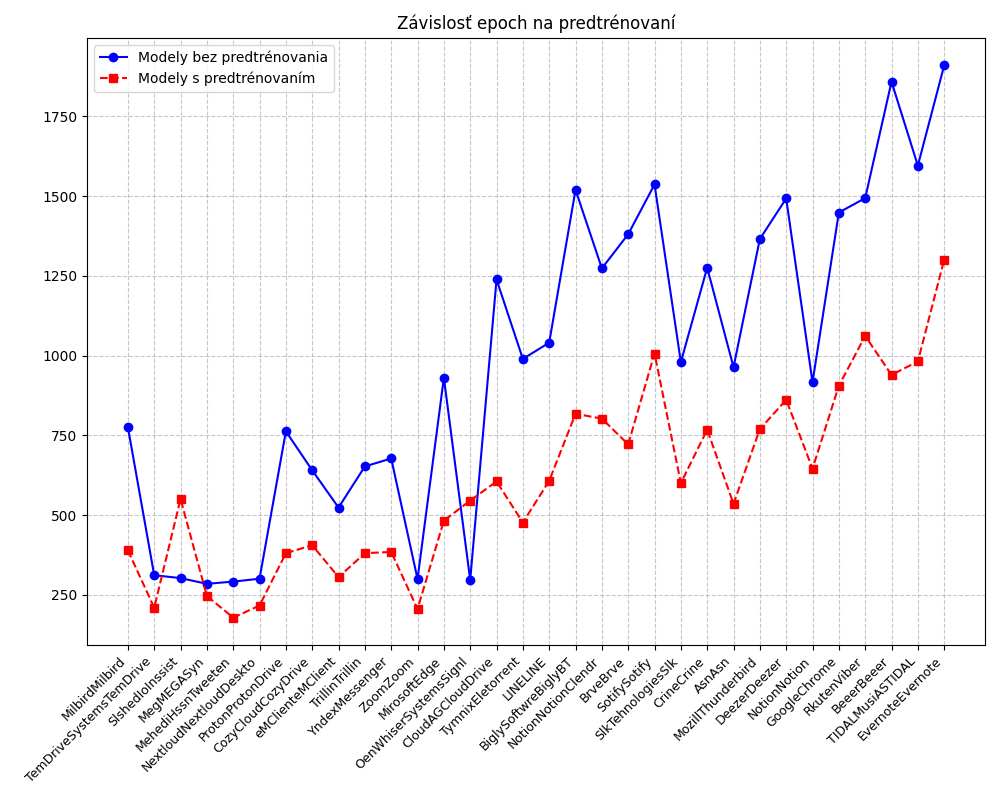
\includegraphics[width=0.9\linewidth]{obrazky-figures/PTEpochs.png}
    \caption{Graf vplyvu predtrénovania na~tréning modelov s~nižším počtom spojení cieľovej aplikácie v~dátovej sade.}
    \label{graph:PTEpochs}
\end{figure}

Pri analýze celkovej úspešnosti boli hodnoty pre~metriky ako precíznosť, presnosť, F1 score a~MCC takmer identické vzhľadom na~nízku variabilitu a~počet TLS spojení pre~dané aplikácie. Zmena bola viditeľná hlavne v~nastavení prahu pre~identifikáciu danej apliokácie, ktoré je viditeľné na~grafu~\ref{graph:PTThreshold}. Z grafu je vidieť, že~väčšina predtrénovaných modelov má prah pre~rekonštrukciu a~rozhodnutie medzi cieľovou a~cudzou aplikáciou nastavený nižšie. Toto znamená, že~model má menší rozptyl rekonštrukčnej chyby a~je vnútorne stabilnejší, čo mu umožňuje stanoviť si prísnejšiu hranicu medzi normálnou prevádzkou a~anomáliou bez toho, aby bol negatívne ovplyvnený šumom v~malých datasetoch.
 \begin{figure}[ht]
    \centering
    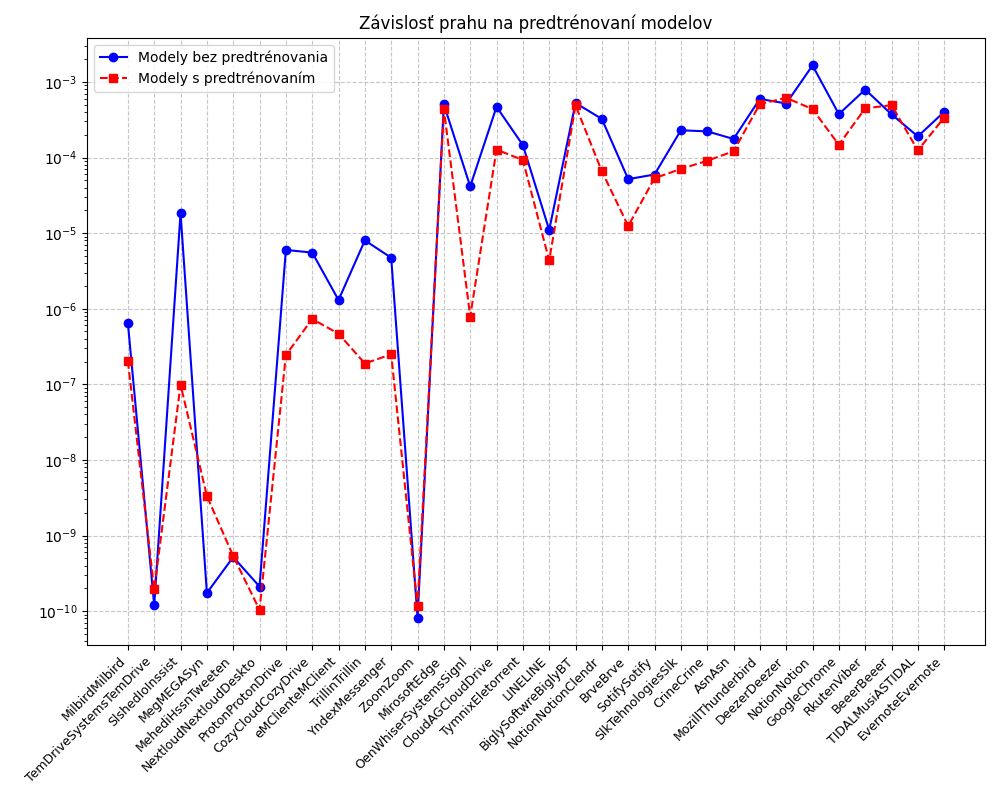
\includegraphics[width=0.9\linewidth]{obrazky-figures/PTThreshold.png}
    \caption{Graf vplyvu predtrénovania na~prah modelov s~nižším počtom spojení cieľovej aplikácie v~dátovej sade.}
    \label{graph:PTThreshold}
\end{figure} 

Odlišnosť vykazovala aj metrika Recall, ktorá pri~modeloch trénovaných od~nuly vykazovala značnú nestabilitu s~hlbokými prepadmi pri~špecifických aplikáciách, zatiaľ čo~predtrénované modely si dokázali udržať vyrovnanejší výkon. Zmeny je možné sledovať na~grafe~\ref{graph:PTRecall}.

Finálne sme sa~v~tejto práci rozhodli využívať predtrénovanie modelov na~zlepšenie konzistentnosti dát a~lepšie všeobecné pochopenie celkovej štruktúry TLS parametrov. V~ďalších sekciach budú experimenty používať tento spôsob trénovania.

\begin{figure}[H]
    \centering
    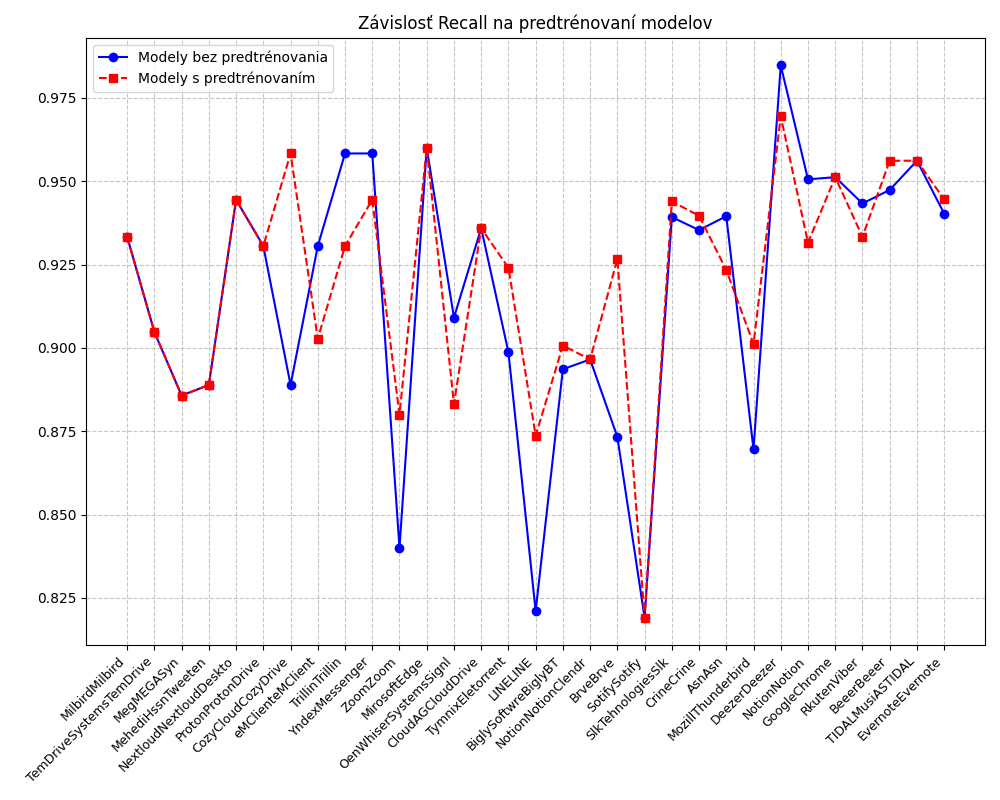
\includegraphics[width=0.9\linewidth]{obrazky-figures/PTRecall.png}
    \caption{Graf vplyvu predtrénovania na~Recall metriku modelov s~nižším počtom spojení cieľovej aplikácie v~dátovej sade.}
    \label{graph:PTRecall}
\end{figure}

\section{Hľadanie ideálnej štruktúry autoenkodéra}\label{exp:architecture}
Autoenkodéry ako každé neurónové siete sú závislé nielen od~svojej kapacity, ale aj od~dát, ktoré sú im sprostredkované. Limitujúcim fakotrom pre~dostupnú dátovú sadu (uvedenú v~tabuľke~\ref{tab:app_connections}) je nižšia veľkosť pre~vstup do~nerónovej siete. Neurónové siete si totiž vyžadujú väčší vstup dát pri~vyššej kapacite, a~preto sa~vybrali aplikácie s~najväčším zastúpením v~dátovej sade. 

Najviac zastúpenou aplikáciou bola AirDroid, ktorá taktiež obsahuje najviac variabilné hodnoty pre~SNI, ktorý má najväčšie zastúpenie v~zakódovaných parametrov. Zaujímavým zistením je, že~hoci aplikácia vykazuje vysoký počet spojení, parametre ako CipherSuite (2) a~Extensions (3) zostávajú relatívne konštantné. To potvrdzuje predpoklad, že~konkrétna verzia klientskej aplikácie používa fixnú knižnicu pre~TLS handshake, zatiaľ čo cieľové domény a~porty sa~dynamicky menia podľa aktuálnej potreby služby. Okrem aplikácie AirDroid boli do~analýzy zahrnuté aj aplikácie OerOer, BiduTerBox a~AdmntMessenger. Aplikácie disponujú počtom vzoriek väčším ako 1000, pričom obsahujú odlišné distribúcie sieťových parametrov, čo umožňuje otestovať robustnosť modelu v~rôznych scenároch.

\begin{table}[H]
    \centering
    \caption{Zúžený prehľad unikátnych TLS parametrov pre~aplikácie s~najväčším počtom TLS spojení}
    \label{tab:app_unique_params}
    \begin{tabular}{lrrrrr}
        \toprule
        \textbf{Aplikácia} & \textbf{SNI} & \textbf{SrcPort} & \textbf{CipherS.} & \textbf{Ext.} & \textbf{Groups} \\ 
        \midrule
        AirDroidAirDroid   & 43 & 149 & 2 & 3 & 17 \\
        OerOer             & 24 & 185 & 3 & 5 & 17 \\
        BiduTerBox         & 21 & 168 & 3 & 4 & 18 \\
        AdmntMessenger     & 23 & 115 & 1 & 3 & 16 \\
        OenMedi4KStogrm    & 27 & 109 & 1 & 2 & 16 \\
        OenMedi4KTokkit    & 27 & 113 & 1 & 2 & 16 \\
        TemSonrrSonrr      & 14 & 92  & 2 & 3 & 17 \\ 
        \bottomrule
    \end{tabular}
\end{table}

\subsubsection{Počet vrstiev}
V tejto časti sa~experimentuje s~počtom skrytých vrstiev, ktoré model obsahuje. Počet vrstiev sa~definuje pre~enkodér, pričom dekodér má \textbf{vždy} štruktúru vrstiev definovanú ako zrkadlový obraz enkodéra. Veľkosť latentného priestoru sa~pre~experimenty spočiatku odhadla okolo 10 až 20 dimenzií, preto sa~zvolila počiatočná veľkosť 16. Konfigurácia ES sa~mierne zmodifikovala, keďže komplexnejšie modely s~viacerými vrstvami sa~optimalizovali pomalšie s~menšími krokmi. Toto bolo spôsobené problémom, ktorým trpia autoenkodérmi nazývaným \textit{\textbf{vanishing gradient}} (miznúci gradient)~\cite{mienye2025deep}. Ako bolo vysvetlené v~sekcii~\ref{th:optim}, gradient sa~počíta pomocou reťazového pravidla, pri~ktorom môže pri~nízkych hodnotách nastať situácia, že~gradient propagujúci sa~do~nižších vrstiev postupne nadobúda limitne nulovú hodnotu. Modifikácia ES tu spočíva v~zmierňovaní podmienky pre~zastavenie tréningu, konkrétne \textbf{dynamickou}\label{exp:dynamic_delta} zmenou \texttt{min\_delta} a~nastavením minimálneho počtu epoch pre~stabilizáciu tréningu. Dynamická zmena pre~\texttt{min\_delta} je vyjadrená vzťahom:
\begin{equation}
    min\_delta = \frac{base\_delta}{\sqrt{N + 1}}
\end{equation}
\begin{itemize}
    \item $base\_delta$: Vyjadruje počiatočne nastavenú minimálnu zmenu pre~ES v~konfigurácii. Experimentálne sa~nastavila najstabilnejšia nájdená hodnota $5\times10^{-6}$.
    \item $N$: Predstavuje počet skrytých vrstiev modelu. 
\end{itemize}
Pre všeobecný model sa~\texttt{min\_delta} zväčší 50-krát, aby prenos učenia na~všeobecných vzorkách slúžil ako fáza hrubej inicializácie váh neurónovej siete. 

S týmito nastaveniami v~skripte \texttt{train\_model\_variants.py} sa~trénovali vybrané aplikácie, pričom sa~vyskúšali veľkosti modelu od~2 až do 8 vrstiev (0 až 6 \textbf{skrytých} vrstiev). Pre~vytváranie vrstiev modelov bolo nastavené proporcionálne rozloženie veľkostí popísané v~sekcii~\ref{imp:proportional}. Ďalšie experimentálne zvyšovanie hĺbky modelu neviedlo k~nárastu presnosti, ako je možné vidieť na~grafoch v~prílohe~\ref{append:layers_structs_graph} alebo na~obrázku~\ref{graph:AirDroidLayersExample}. Analýza závislosti MCC a~počtu epoch od~počtu vrstiev modelu potvrdzuje existenciu bodu nasýtenia (koncu výraznej konvergencie modelu pri~tréningu). Zatiaľ čo zvyšovanie počtu vrstiev z~2 na~4 prináša zlepšenie klasifikačnej schopnosti modelu (MCC rastie z~$0,2$ na~$0,53$), ďalšie prehlbovanie siete (nad 5 vrstiev) vedie k~nárastu výpočtovej náročnosti tréningového procesu. Počet potrebných epoch sa~po prekročení 5. vrstvy zdvojnásobil, bez zaznamenania výrazného nárastu metriky MCC. Z hľadiska efektivity tréningu a~komplexnosti modelu sa~preto ako optimálna javí 4-vrstvová alebo 5-vrstvová architektúra, ktorá predstavuje ideálny balans medzi presnosťou modelu a~náročnosťou jeho tréningu.

\begin{figure}[H]
    \centering
    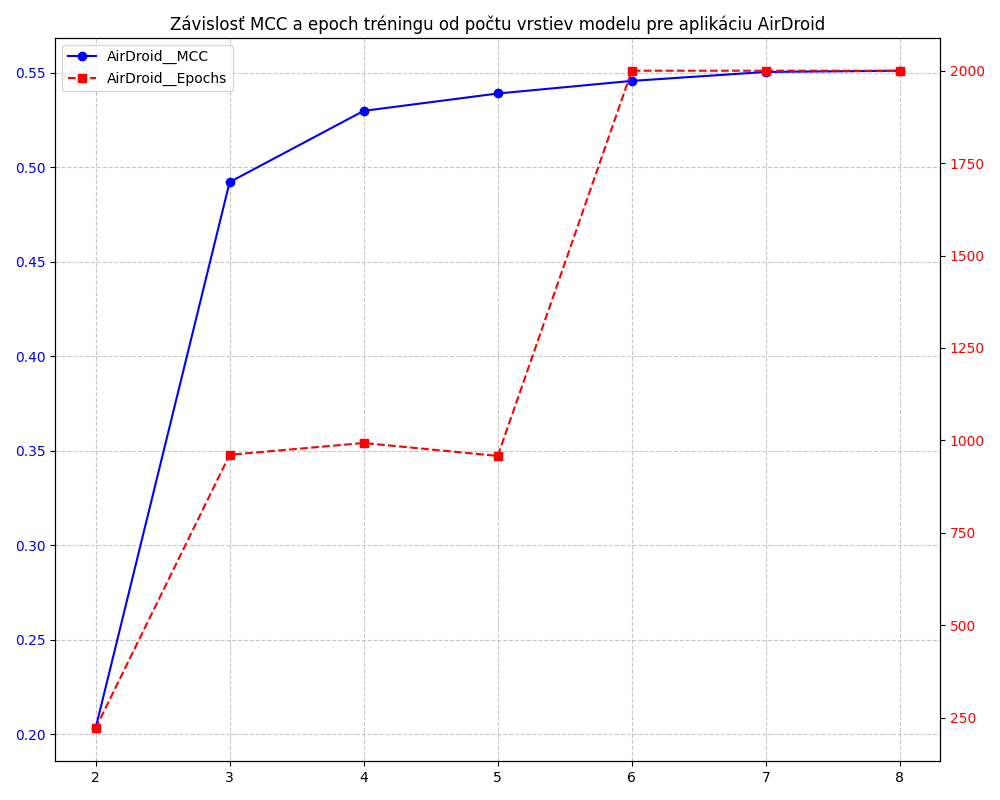
\includegraphics[width=0.5\linewidth]{obrazky-figures/AirDroidMCC.png}
    \caption{Ukážka vplyvu vrstiev na~úspešnosť a~efektivitu tréningu pre~aplikáciu AirDroid}
    \label{graph:AirDroidLayersExample}
\end{figure}

\subsubsection{Veľkosť latentnej vrstvy}\label{exp:latent}
Po určení optimálneho počtu vrstiev bolo cieľom experimentov zistiť vplyv veľkosti latentného priestoru na~presnosť klasifikácie. Latentná vrstva predstavuje najužšie miesto siete, ktoré núti model komprimovať vstupné príznaky do~reprezentatívnej formy. Pre~tento test boli zvolené architektúry so 4, 5 a~6 vrstvami, pričom veľkosť \textit{bottlenecku} sa~menila v~rozsahu od~8 do~20 neurónov. Z výsledkov testu viditeľných v~prílohe~\ref{graph:latent_size_graphs} alebo v~ukážke~\ref{fig:combined_latent_analysis} je možné vidieť, že~hodnoty 12, 14 a~16 sa~javia ako najstabilnejšie. Modely od~6 vrstiev, ako bolo ukázané v~sekcii~\ref{exp:pre-training}, potrebujú veľký počet epoch pre kvalitný tréning a~zabránenie javu \textit{vanishing gradient}, čo je vidieť aj v~ukážkach~\ref{graph:Latent6MCC},~\ref{graph:Latent6F1} pre~model so 6 vrstvami. Modely s~počtom vrstiev 4 a~5 majú relatívne nízky počet epoch po~latentný priestor veľkosti 14 dimenzií, a~teda z~tohoto pohľadu je veľkosť 14 najlepšia varianta.

\begin{figure}[H]
    \centering
    \begin{subfigure}[b]{0.48\textwidth}
        \centering
        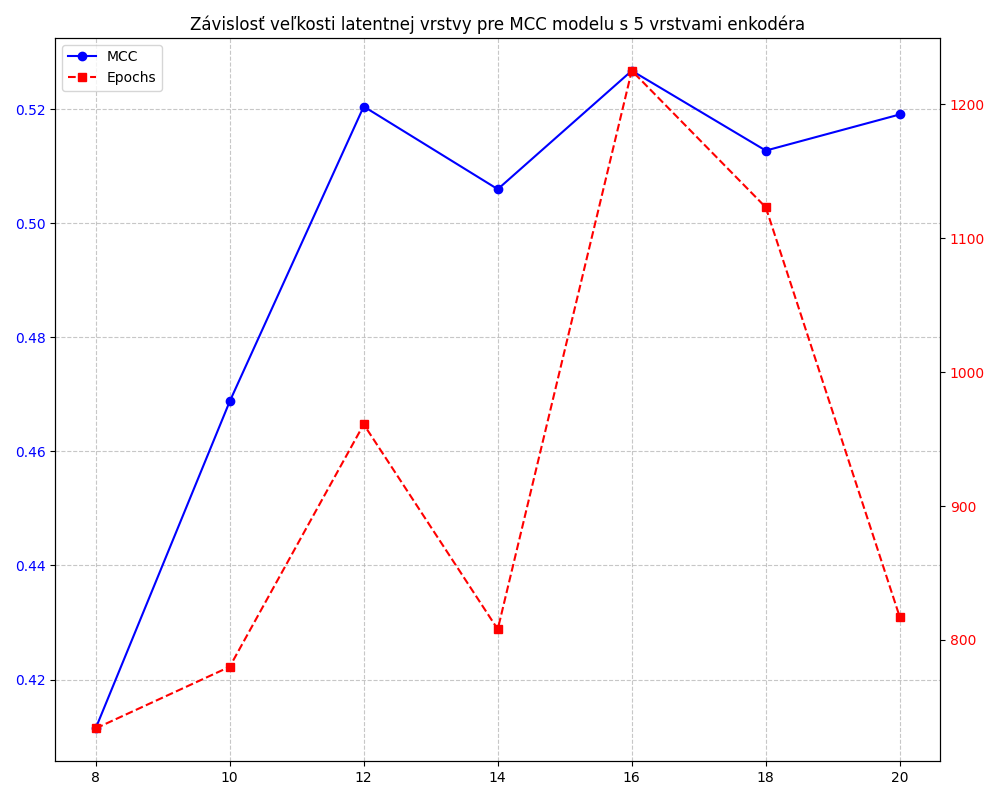
\includegraphics[width=\textwidth]{obrazky-figures/Latent5.png}
        \caption{Vplyv veľkosti \textit{bottlenecku} na~MCC.}
        \label{graph:5LayersMCCExample}
    \end{subfigure}
    \hfill
    \begin{subfigure}[b]{0.48\textwidth}
        \centering
        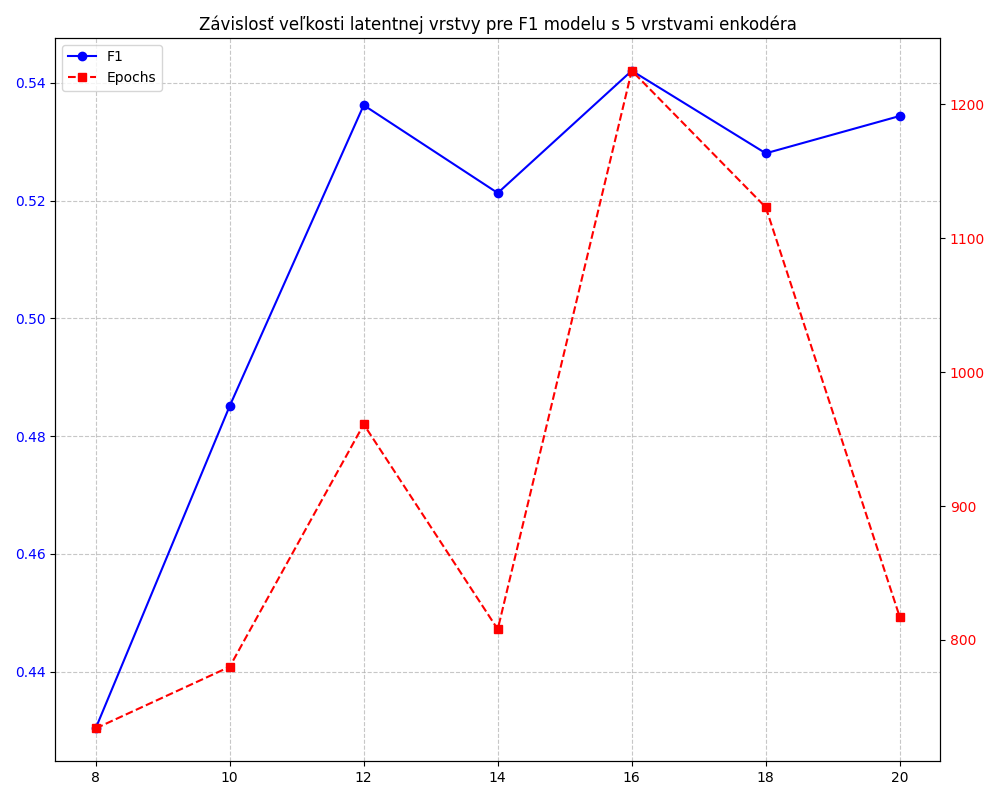
\includegraphics[width=\textwidth]{obrazky-figures/Latent5F1.png}
        \caption{Vplyv veľkosti \textit{bottlenecku} na~F1.}
        \label{graph:5LayersF1Example}
    \end{subfigure}
    \caption{Analýza parametrov pre~5-vrstvový model:..}
    \label{fig:combined_latent_analysis}
\end{figure}

Ako je uvedné v~sekcii~\ref{des:mcc}, 
MCC koeficient berie ohľad na~všetky polia \textit{confusion matrix}. F1 skóre sa~líši od~tohto koeficientu práve tým, že~neberie do~úvahy pole \textit{True Negative} (TN). Z grafov v~prílohe~\ref{graph:latent_size_graphs} alebo v~ukážke~\ref{fig:combined_latent_analysis} je možné vyčítať, že~metriky F1 a~MCC majú takmer identický priebeh grafu, čo znamená, že~počet TN, ktorý F1 skóre vynecháva, je v~rámci klasifikácie stabilne vysoký a~model tak vykazuje minimálnu chybovosť pri~identifikácii necieľových aplikácií. Z grafov v~prílohe~\ref{graph:latent_size_graphs_Precision} alebo v~ukážke~\ref{graph:5LayerPrecisionRecallExample} pre~5-vrstvový model je možné vidieť závislosť metrík precision a~recall. Tieto metriky úzko súvisia s~výpočtom MCC a~F1, práve ktorými hodnotíme úspešnosť modelu. Z testovaní je~zrejmé, že~metrika recall má pre~všetky modely stabilné a~pozitívne výsledky, narozdiel od~metriky precision, ktorej zmeny podľa vrstiev sú rádovo väčšie. Metrika precision dosahovala nízke hodnoty, ktoré nepresiahli 50\,\%, a~práve preto táto metrika ovplyvňuje úspešnosť modelu najviac. Z uvedeného vyplýva, že~model vykazuje vysokú mieru pokrytia cieľových aplikácií, avšak za~cenu nižšej miery spoľahlivosti jednotlivých predikcií.

\begin{figure} [H]
    \centering
    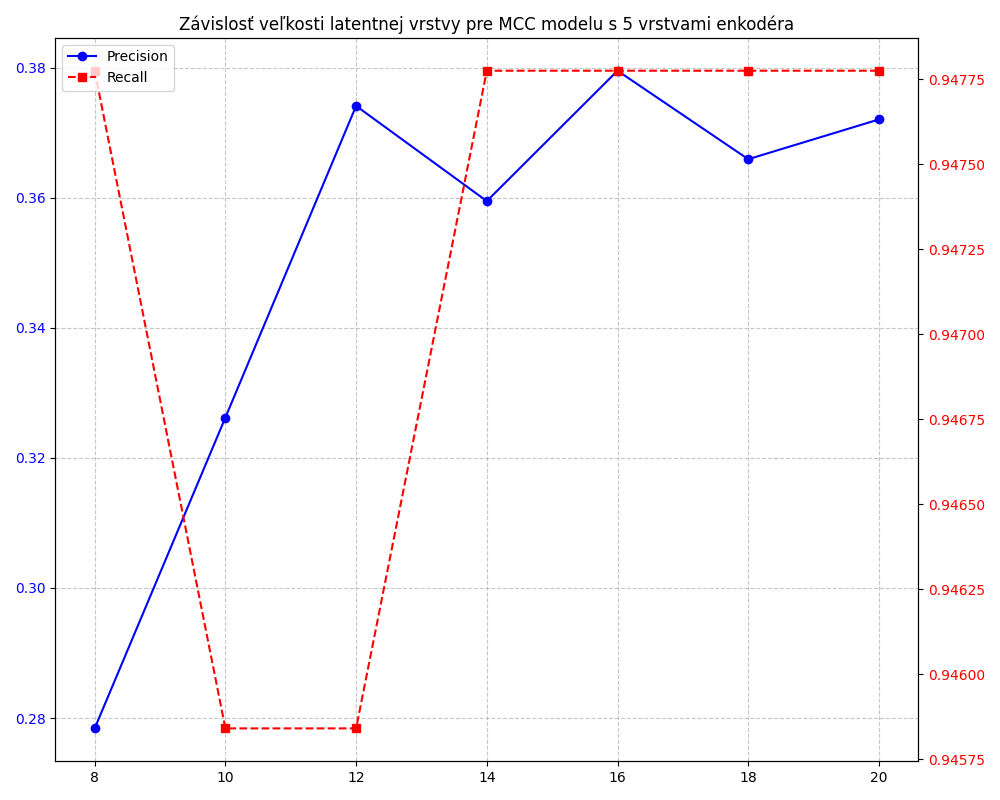
\includegraphics[width=0.5\linewidth]{obrazky-figures/PrecisionRecall5.png}
    \caption{Ukážka závislosti Precision a~Recall od~veľkosti \textit{bottlenecku} pre~5-vrstvový model.}
    \label{graph:5LayerPrecisionRecallExample}
\end{figure}

\section{Testovanie modifikácie prahovej hodnoty}
V predchádzajúcej sekcii sme určili ako hlavný problém zníženej úspešnosti autoenkodérov nízku precision. Tento problém je spôsobený nielen len vysokou variabilitou TLS parametrov zvolenej cieľovej aplikácie (AirDroid), ale aj vysokou pravdepodobnosťou zhody TLS parametrov pre~TLS spojenia iných aplikácie. V~tejto sekcii sa~snažíme experimentálne zúžovať hranicu medzi množinou cieľových a~cudzích aplikácií za~účelom zvýšenia pravdepodobnosti, že~rekonštrukčná chyba pre~cudzie aplikácie bude väčšia ako určený prah pre~natrénovaný model. Trénovaný model mal štruktúru 182-140-98-56-14, čo znamená, že~obsahoval 5 vrstiev neurónov (3 skryté) s~veľkosťou latentného priestoru 14. Po natrénovaní sa~vykonaly testy, kde pri~každom teste sa~znižovala hodnota prahu, s~ktorým model binárne klasifikuje množinu vstupných dát. Prah sa~znižoval postupne o 5\,\% základného prahu, pričom sa~pokračovalo týmto spôsobom až do~50\,\% základného prahu. 

Výsledky testov je možné vidieť na~grafe~\ref{graph:AirDroidThreshold}. So znižujúcim prahom sa~skutočne zvyšuje metrika precision, avšak pochopiteľne na~úkor recall. Recall sa~v~tomto prípade radikálnejšie znišuje, čo je pravdepodobne spôsobené väčším podielom cudzích TLS spojení aplikácií v~testovacích dátach. Táto nevyvážená nepriama úmera je pozorovateľná na~grafe~\ref{graph:AirDroidThresholdMCC}, kde koeficient úspešnosti MCC postupne klesá. Na~základe uvedených faktov je najlepšou voľbou zníženie prahu na~rozsah hodnôt 90 až 85\,\%.

\begin{figure}[H]
    \centering
    \begin{subfigure}[b]{0.48\textwidth}
        \centering
        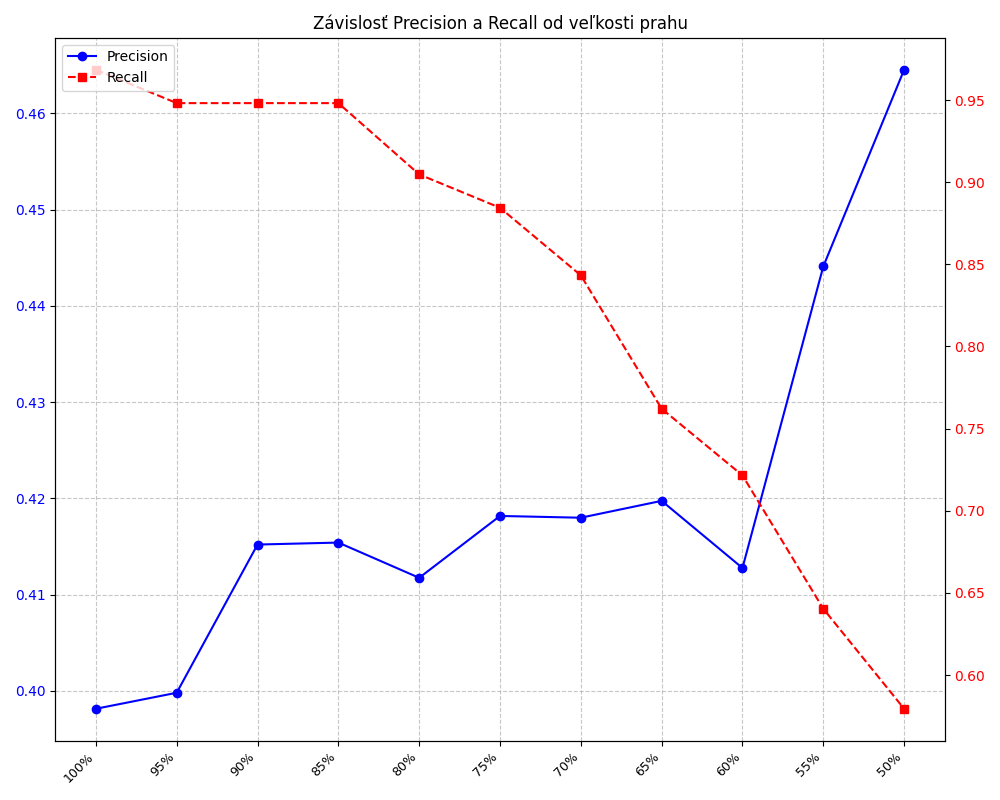
\includegraphics[width=\textwidth]{obrazky-figures/AirDroidThreshold.png}
        \caption{Vplyv prahu na~precision a~recall.}
        \label{graph:AirDroidThreshold}
    \end{subfigure}
    \hfill
    \begin{subfigure}[b]{0.48\textwidth}
        \centering
        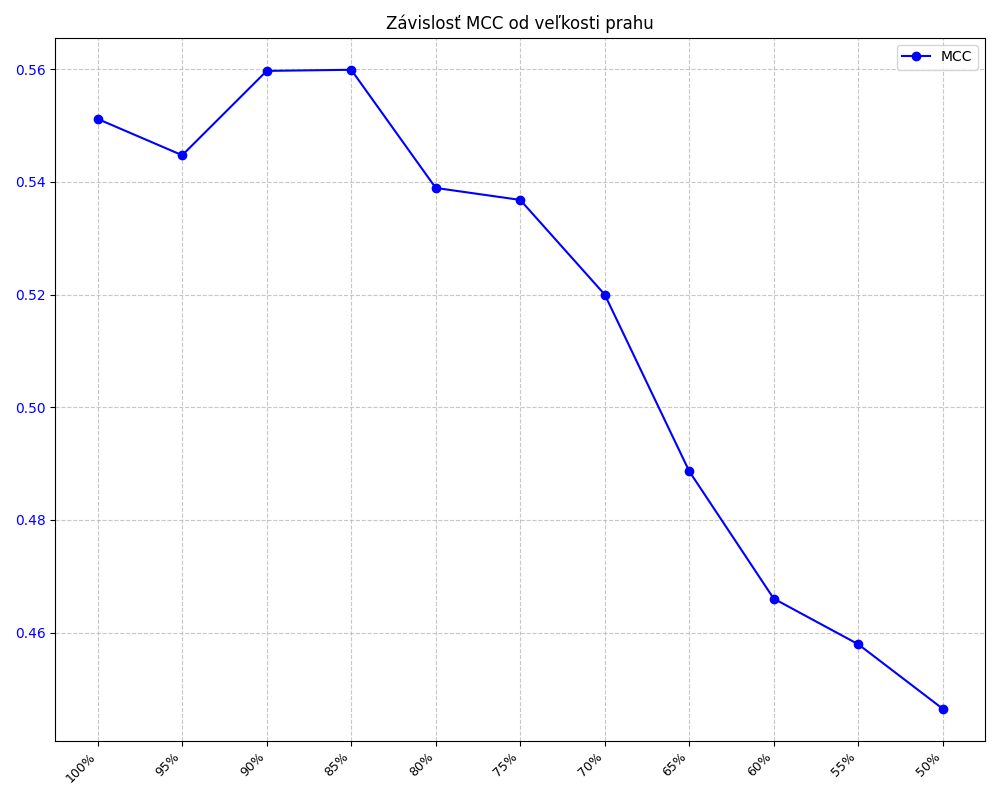
\includegraphics[width=\textwidth]{obrazky-figures/AirDroidThresholdMCC.png}
        \caption{Vplyv prahu na~MCC.}
        \label{graph:AirDroidThresholdMCC}
    \end{subfigure}
    \caption{Analýza vplyvu zníženia prahu pre~model aplikácie AirDroid so štruktúrou 182-140-98-56-14.}
    \label{fig:combined_threshold}
\end{figure}

\section{Klasifikácia s~viacerými modelmi}
V tejto sekcii sa~bude analyzovať úspešnosť systému viacerých autoenkodérov, pričom sa~snažíme zvýšiť výkonnosť vzhľadom na~klasifikáciu s~použitím iba jedného modelu. Budeme experimentovať s~výkonnosťou systému pri~binárnej klasifikácii a~viactriednej klasifikácii. 

\subsection{Binárna klasifikácia s~využitím viacerých modelov}\label{exp:binary}
V tejto časti sa~zameriame na~testovanie systému zloženého z~viacerých modelov identifikujúcich TLS spojenia pre~svoju aplikáciu, pričom sa~zameriame na~klasifikáciu iba jednej z~nich. Týmto prístupom chceme zaviesť mechanizmus prirodzenej filtrácie: vzorky cudzej prevádzky, ktoré by pri~použití samostatného modelu generovali falošne pozitívne detekcie (FP), sú v~tomto prípade priradené relevantnejšiemu modelu. Týmto spôsobom chceme znížiť hlavný problém nižšej úspešnosti modelu -- nízka precíznosť. Do systému budeme postupne pridávať modely jednotlivých aplikácii v~poradí, akom sú uvedené v~grafe~\ref{graph:ModelsMCC}, ktorý reprezentuje ich jednotlivú výkonnosť. Ďalšie metriky modelov sú uvedené v~tabuľke~\ref{tab:each_model_all_metrics}. 

\begin{figure}[ht]
    \centering
    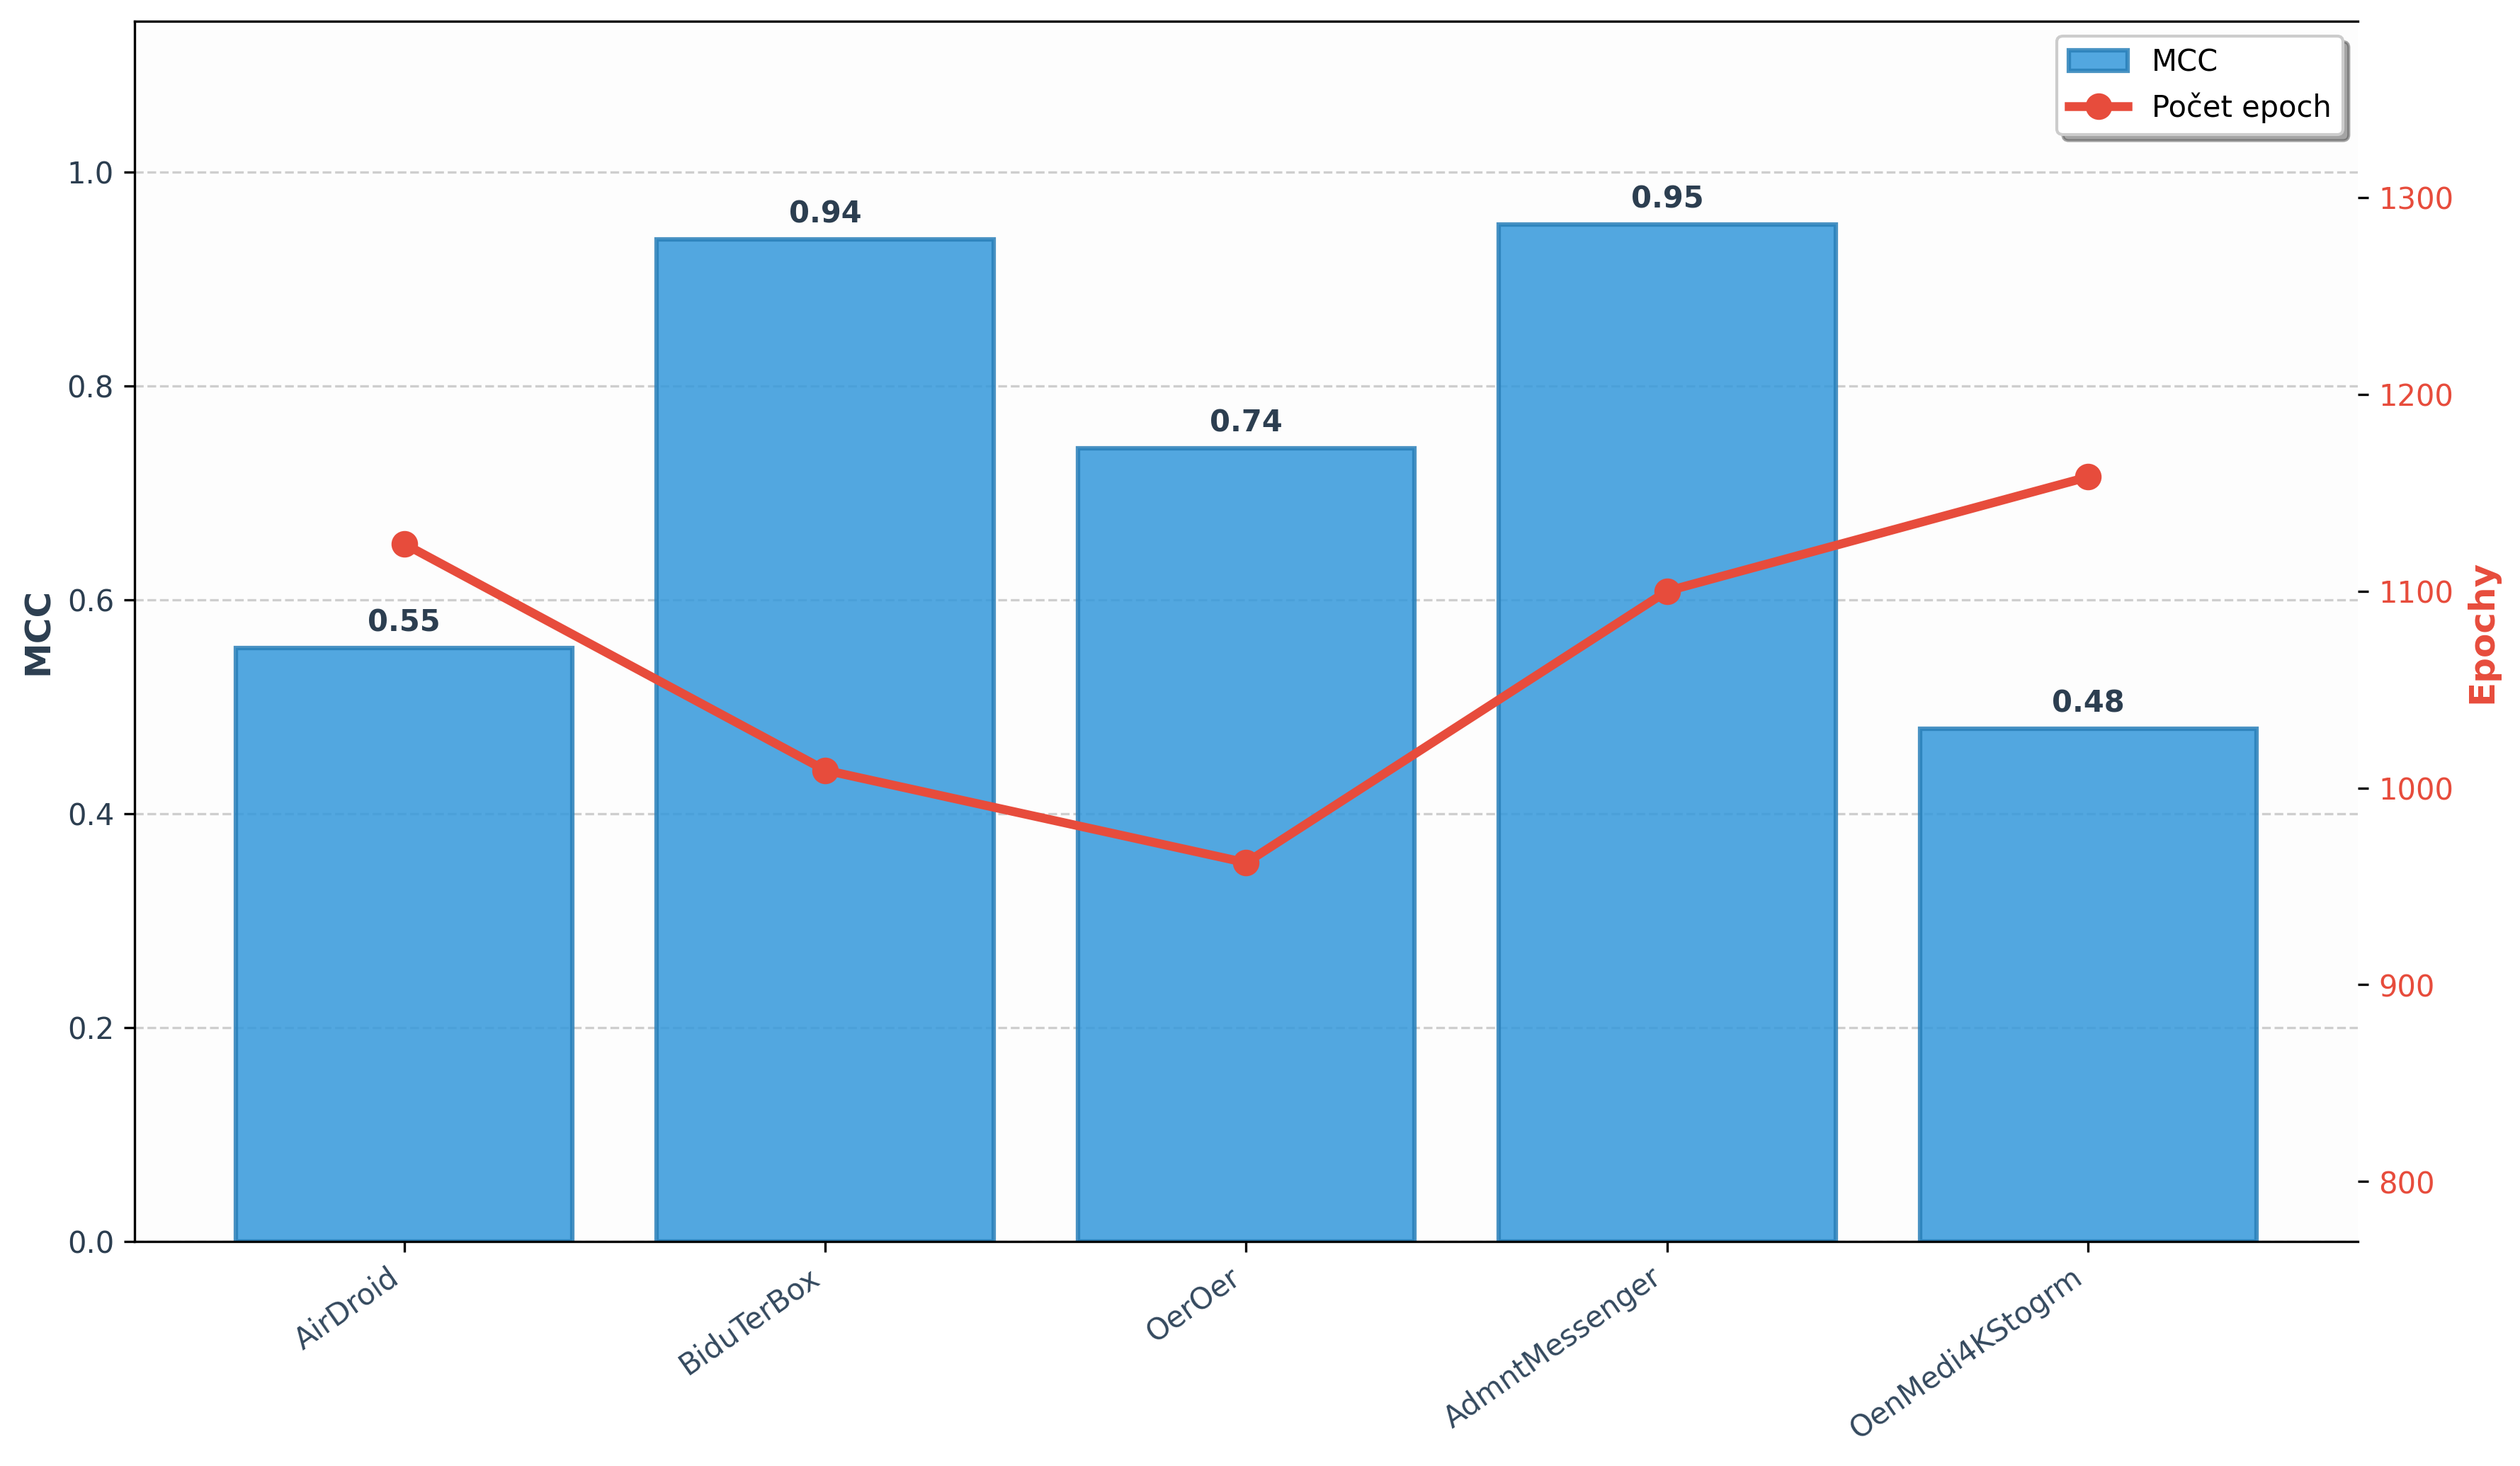
\includegraphics[width=0.8\linewidth]{obrazky-figures/MultipleModelsMCC.png}
    \caption{Výkonnosť jednotlivých modelov so štruktúrou 182-140-98-56-14, ktoré sa~používajú v~tomto teste.}
    \label{graph:ModelsMCC}
\end{figure}
Výsledok testov je možné vidieť na~grafoch~\ref{graph:multiple_binary_test_results}. Pridanie modelov, ako bolo predpokladané, má pozitívny vplyv na~celkovú výkonnosť modelov meranou pomocou koeficientu MCC, čo znamená, že~sa zlepšila metrika precíznosti (precision).

Hoci tento filtračný mechanizmus zvyšuje čistotu detekcie (precision), dochádza k~nemu za~cenu mierneho nárastu falošne negatívnych výsledkov (FN), keďže niektoré vzorky cieľovej aplikácie môžu byť chybne klasifikované konkurenčným modelom s~podobnými charakteristikami váh neurónov. Toto zapríčiňuje pokles metriky recall, ktorý je možný vidieť na~grafe~\ref{graph:MultipleRecall}. Pridávanie ďalších modelov do~systému hodnotíme, aj napriek poklesu senzitívnosti, ako pozitívny prínos, hlavne vďaka zlepšeniu hodnôt pre~koeficient MCC.

\begin{figure}[H]
    \centering
    \begin{subfigure}[b]{0.48\textwidth}
        \centering
        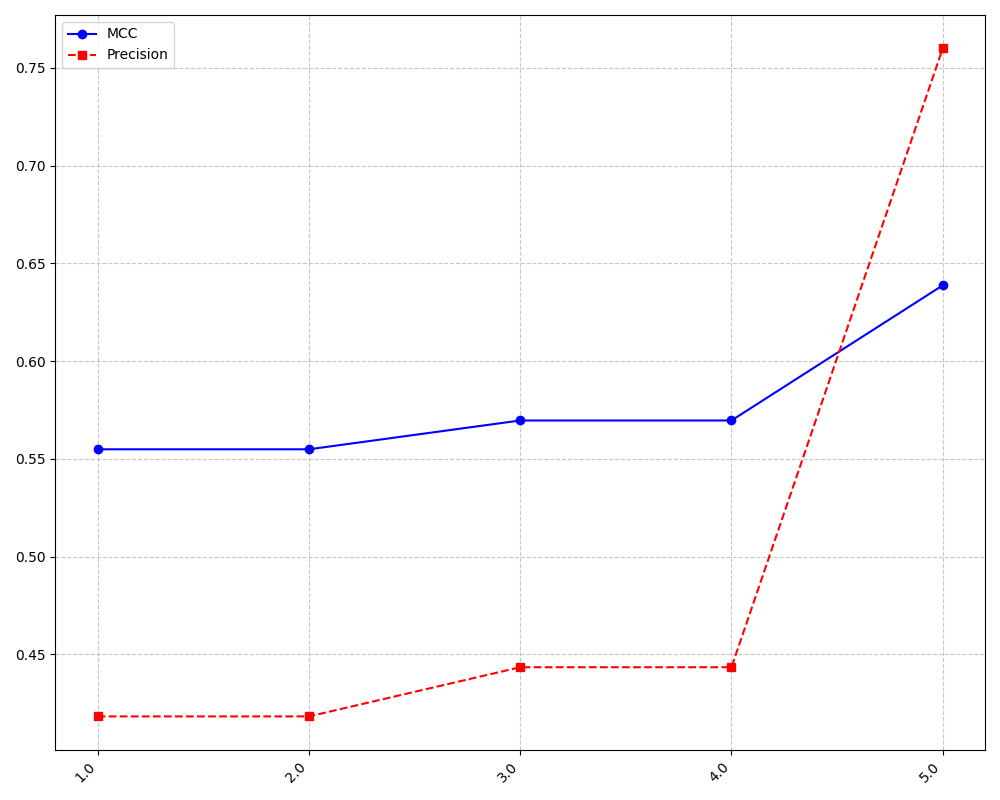
\includegraphics[width=\textwidth]{obrazky-figures/MultipleBinaryMCC.png}
        \caption{Vplyv počtu modelov na~MCC a~precision.}
        \label{graph:MultipleBinaryMCC}
    \end{subfigure}
    \hfill
    \begin{subfigure}[b]{0.48\textwidth}
        \centering
        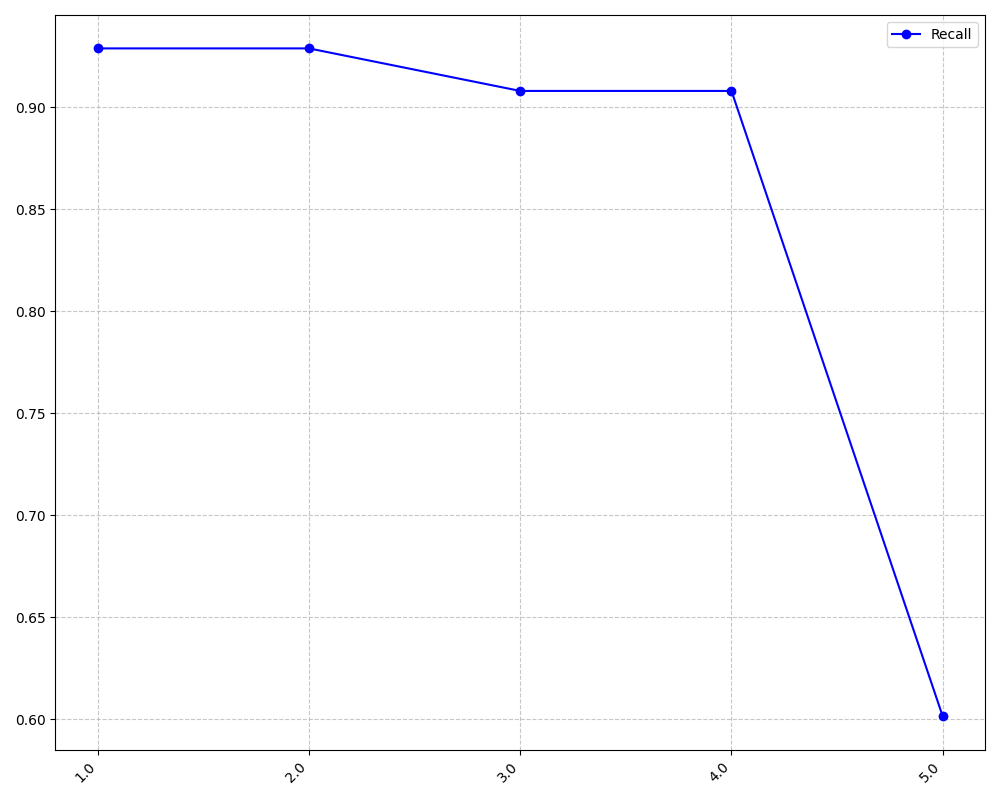
\includegraphics[width=\textwidth]{obrazky-figures/MultipleBinaryRecall.png}
        \caption{Vplyv počtu modelov na~recall.}
        \label{graph:MultipleRecall}
    \end{subfigure}
    \caption{Výsledky testov využitia viacerých modelov pre~binárnu klasifikáciu.}
    \label{graph:multiple_binary_test_results}
\end{figure}

\subsection{Viactriedna klasifikácia}
Ako bolo uvedené v~sekcii~\ref{imp:classification}, pri~viactriednej klasifikácii budeme využívať systém OVA, čo znamená, že~klasifikačný systém sa~bude skladať z~binárnych klasifikátorov pre~jednotlivé aplikácie. Pri~testovaní sa~postupne pridávali modely trénované na~klasifikáciu jednotlivých aplikácií, pričom sa~všetky aplikácie klasifikačných modelov označili ako cieľové.  

Pri zvyšovaní počtu modelov sa~znižovala presnosť systému (\textit{accuracy}). Množina cieĺových aplikácií sa~totiž zväčšuje vzhľadom na~celú dátovú sadu a~množina cudzích aplikácií sa~zmenšuje, čo znamená nárast metriky FPR (\textit{false positive rate}). Tento jav je spôsobený faktom, kde zvýšenie počtu modelov v~systéme vytvorí väčšiu šancu na~to, aby sa~klasifikovala ako vzorka pre~jedného z~využitých modelov, práve kvôli problému opísanom v~sekcii~\ref{exp:latent}. Ako je možné vidieť v~grafe~\ref{graph:MultipleACCFPR}, takýmto spájaním modelov do~jedného klasifikačného systému sa~chyba postupne propaguje.   

\begin{figure}[H]
    \centering
    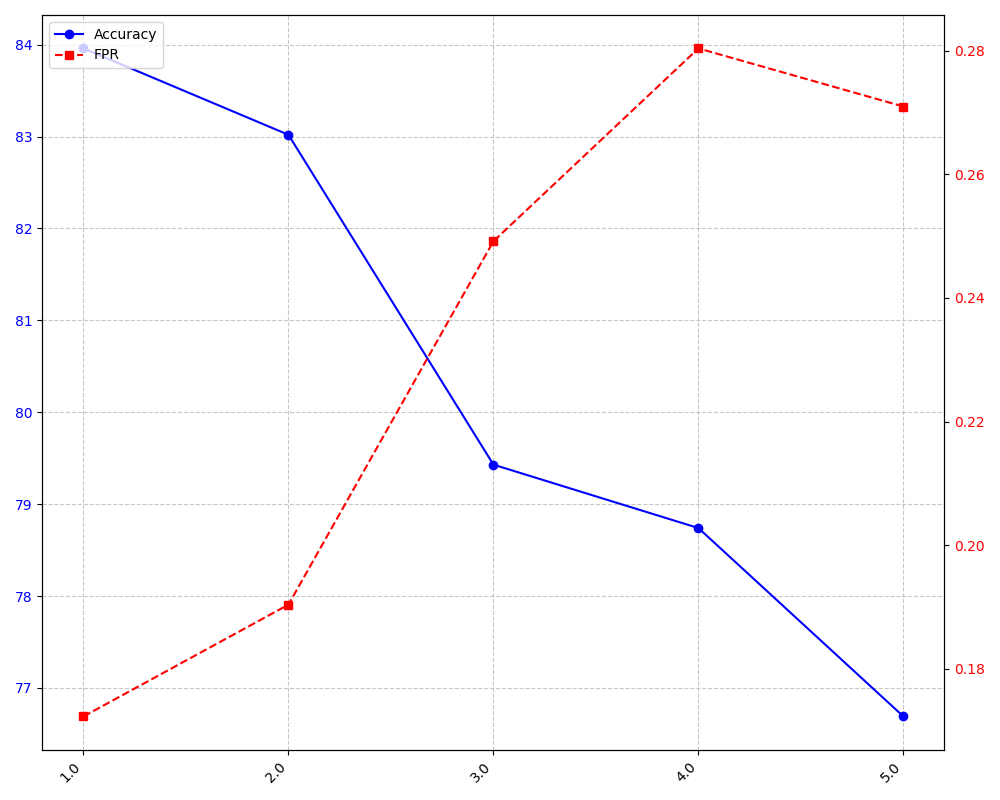
\includegraphics[width=0.7\linewidth]{obrazky-figures/MultipleMulticlassAccFPR.png}
    \caption{Graf ukazujúci vplyv počtu modelov na~metriky accuracy a~FPR.}
    \label{graph:MultipleACCFPR}
\end{figure}

Ako ve uvedené v~sekcii~\ref{exp:binary}, pridávanie modelov zvyšuje precíznosť systému. To môžeme vidieť aj v~prípade viactriednej klasifikácie podľa grafu~\ref{graph:MutliplePreRec}. Metriky \textit{accuracy} (presnosť) a FPR sú navzájom nepriamo úmerné, pričom rozdiel nastáva v~momente, keď model neslúži len ako filter cudzích aplikácií. Modely, ktoré zachytia väčší počet vzoriek z~trénovacích dát, zvyšujú celkový počet správnych detekcií (TP), čím v~prostredí viactriednej klasifikácie kompenzujú straty spôsobené medzimodelovou interferenciou, teda faktom, že~dokážu prebrať klasifikáciu cieľovej aplikácie modelu, ktorý je na~ňu trénovaný.

\begin{figure}[H]
    \centering
    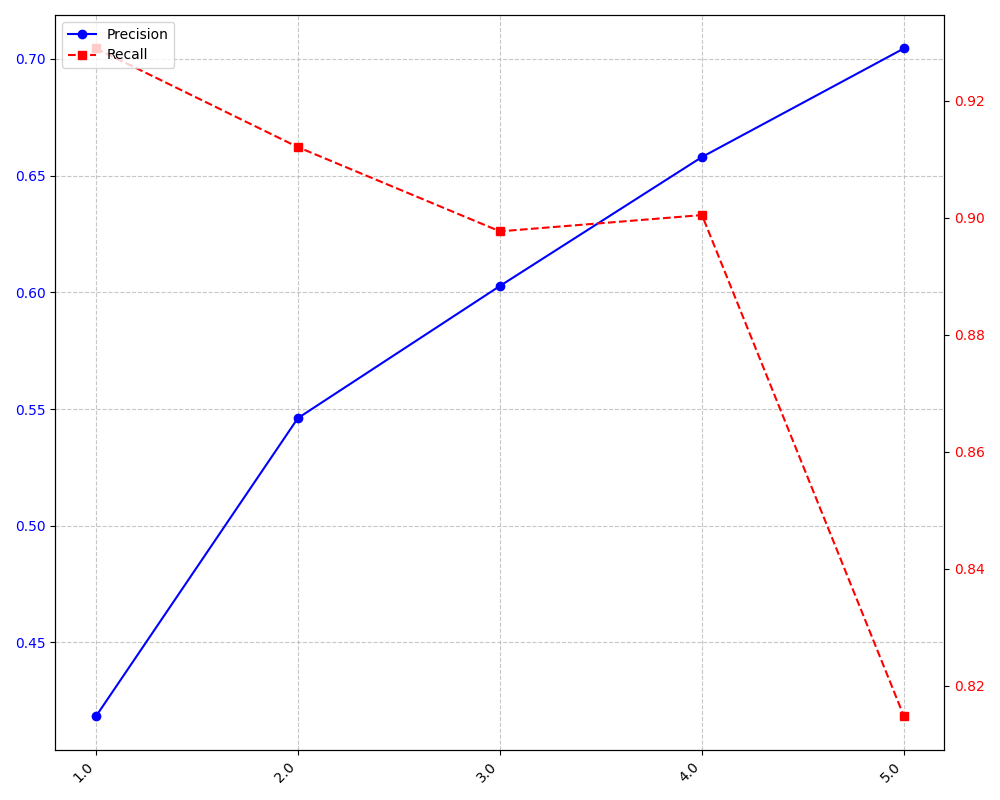
\includegraphics[width=0.7\linewidth]{obrazky-figures/MultipleMulticlassPreRec.png}
    \caption{Graf ukazujúci vplyv počtu modelov na~metriky precision a~recall.}
    \label{graph:MutliplePreRec}
\end{figure}

V poslednom grafe~\ref{graph:MCCF1} je možné vidieť celkovú úspešnosť systému reprezentovanú metrikami F1 a~MCC. Práve tu je jasne vidieť rozdiel medzi F1 skóre a~MCC koeficientom, ktorý hodnotí systém kritickejšie. Nárast F1-skóre je primárne spôsobený rozširovaním cieľovej množiny dát a~výrazným zlepšením precíznosti systému. Keďže F1-skóre sa~zameriava výhradne na~úspešnosť detekcie pozitívnej triedy, odráža narastajúcu schopnosť systému rozpoznávať známe TLS spojenia. Táto metrika však neberie do~úvahy schopnosť systému rozpoznávať cuzdzie TLS spojenia (TN), ktorá je zohľadnená koeficientom MCC. Z grafu je rozpoznateľné, že~hondoty pre~MCC relatívne stagnujú (pri 5. modely dokonca hodnota klesá), čo ukazuje skutočnú výkonnosť klasifikačného systému, ktorá má podobný charakter ako kombinácia výkonnosti jednotlivých modelov (vidieteľný podobný priebeh koeficientu ako na~grafe~\ref{graph:ModelsMCC} reprezentujúci samostatné modely). Kombinácia modelov teda pri~viactriednej klasifikácii neprináša lepšiu výkonnosť systému, ale iba umožňuje rozšírenie jeho \textbf{detekčného spektra} o ďalšie špecifické triedy aplikácií.

\begin{figure}[H]
    \centering
    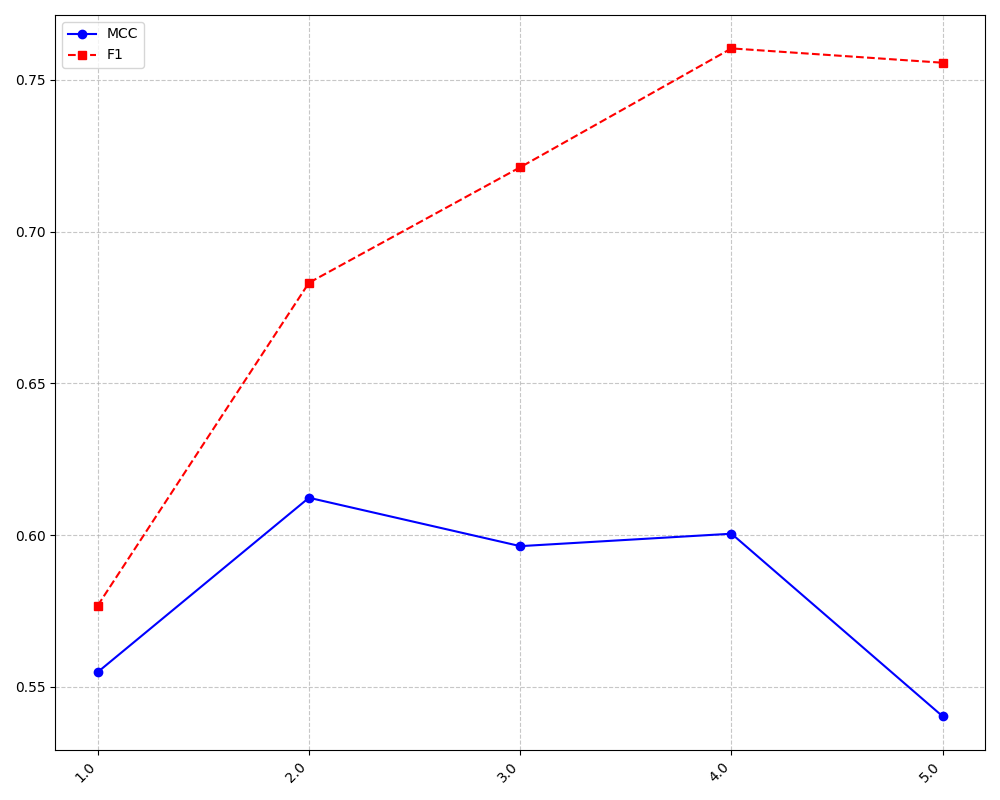
\includegraphics[width=0.7\linewidth]{obrazky-figures/MultipleMulticlassMCCF1.png}
    \caption{Graf ukazujúci vplyv počtu modelov na~metriky MCC a~F1.}
    \label{graph:MCCF1}
\end{figure}

\section{Porovnanie s~exitujúcimi riešeniami}
Pri porovnaní s~výsledkami publikovanými v~štúdii~\cite{app_identification} je potrebné rozlišovať medzi metodikou vyhodnocovania. Nami navrhnutý systém pridáva triedu neznámej aplikácie, pri~ktorej sa~tiež vyhodnocuje úspešne a~neúspešné priradenie, pričom štúdia sa~snaží každú aplikáciu vždy priradiť k~známej triede a~neznámu aplikáciu jednoducho nezaraďuje (neprispieva k~pozitívnej alebo negatívnej predikcii).

Štúdia prezentuje výsledky pre~multiclass klasifikáciu, kde dosahuje Accuracy v~rozsahu 75\,\% až 86,3\,\% (pre SNI identifikáciu) a~F1-skóre blížiace sa~k~hodnote 0,9. Nami navrhnutý systém viacerých autoenkodérov dosahuje v~multiclass scenári (pri použití 5 modelov s~najväčším zastúpením svojich cieľových aplikácií) F1-skóre 0,76, čo je hodnota porovnateľná s~metódami identifikácie s~využitím JA4+JA4S (presnosť 54\,\% až 80\,\%) uvedenými v~referenčnej štúdii. Môžeme teda potvrdiť, že~použitie autoenkodérov pri~\textbf{\textit{multiclass}} klasifikácii dosahuje výsledky porovnateľné s~metódami v~referenčnej štúdii, pričom sa~nejaví ako najlepšia možnosť, ale je použiteĺný v~reálnej sieťovej prevádzke. Menšia výkonnosť môže byť spôsobená práve aj zavedením korektnosti identifikácie neznámych aplikácii, čo reprezentuje MCC koeficient, ktorý v~štúdii uvedený nie je.

\chapter{Záver}
Cieľom tejto bakalárskej práce bola identifikácia aplikácií na~základe ich inicializačných parametrov pre~TLS spojenie s~využitím autonkodérových neurónových sietí. Návrh a~implementácia riešenia mala priniesť čo najpresnejší systém klasifikácie, pričom bola predstavená nielen binárna klasifikácia s~využitím jednotlivých modelov, ale aj viactriedna klasifikácia, ktorá sa~realizovala kombináciou viacerých modelov.

Práca sa~zaoberala najskôr analýzou a~spracovaním dát, pričom spôsob transformácie dát do~vektorovej podoby sa~prejavil ako efektívny a~relatívne úspešný pre~reprezentáciu aplikácií v~jednotnej číselnej podobe normalizovanej okolo 0. Rozdelenie váh dát pre~jednotlivé TLS parametre vychádzali z~úspešnosti jednotlivých metód z~referenčnej štúdie~\cite{app_identification} a~z~významu ich hodnoty. Ďalej práca navrhla a~implementovala klasifikačný systém s~využitím autoenkodérov, pričom hlavným cieľom tohoto systému bolo nájsť optimálnu štruktúru a~hodnoty pre~dostupnú dátovú sadu. Hodnotenie úspešnosti sa~realizovalo experimentálne zvyšovaním komplexnosti systému pridávaním modelov pre ďalšie aplikácie, pričom sa~bral ohľad na~nevyváženosť dátovej sady, a~teda použité modely boli trénované na~aplikácie s~najväčším zastúpením. 

Navrhnutý spôsob implementácie vykazuje solídne výsledky, kde koeficient MCC ako hlavný indikátor výkonnosti systému dosahoval nadpriemerné hodnoty pre~samostatné modely (viz.~\ref{tab:each_model_all_metrics}). Kombinácia modelov sa~ukázala v~binárnej klasifikácii ako pozitívny prínos pre~klasifikačný systém, kde pri~identifikácii najspoľahlivejšej aplikácie s~najväčším počtom vzoriek je vidieť nárast koeficientu MCC z~hodnoty $0,55$ na~$0,64$. Experimenty ukázali, že~pri viactriednej klasifikácii sa~systém nezlepšuje vďaka vyššiemu počtu modelov v~zmysle zvyšovania kvality predikcie. MCC sa~ustálil na~hodnote, ktorá reflektuje priemernú rozlišovaciu schopnosť jednotlivých modelov tvoriacich systém.

Vysoké hodnoty metriky recall jednotlivých modelov môžu byť kľúčové v~scenároch, kde je prioritou identifikácia relevantných TLS spojení cieľovej aplikácie aj za~cenu nárastu falošných pozitívnych predikcií (FPR). Práve tento princíp poskytujú implementované modely, čo môže byť prínosné pre~monitorovacie systémy, kde by prehliadnutie konkrétnej komunikácie mohlo predstavovať bezpečnostné riziko alebo stratu dôležitých dát.

Prácu je možné doplniť o experimenty so spomínaným \textit{fast text} kódovaním SNI (viz.~\ref{emb:SNI}), kde by bola potrebná širšia dátová sada. Keďže systém spolieha na~TLS parametry, kódovanie vstupných dát by sa~dalo rozšíriť o podporu ECH (\textit{Encrypted Client Hello}) a~ESNI (\textit{Encrypted SNI}), ktoré sa pre~ochranu súkromia používajú čoraz častejšie. Taktiež ďalším krokom by mohlo byť vykonanie testovania na~reálnej sieťovej komunikácii a~overenie funkčnosti systému, keďže v~tejto práci testovanie prebiehalo iba lokálne na~statických dátach.\enlargethispage{\baselineskip}
  \fi
  
  % Kompilace po částech (viz výše, nutno odkomentovat a zakomentovat input výše)
  % Compilation piecewise (see above, it is necessary to uncomment it and comment out input above)
  %\subfile{chapters/projekt-01-uvod-introduction}
  % ...
  %\subfile{chapters/projekt-05-zaver-conclusion}

  % Pouzita literatura / Bibliography
  % ----------------------------------------------
\ifslovak
  \makeatletter
  \def\@openbib@code{\addcontentsline{toc}{chapter}{Literatúra}}
  \makeatother
  \bibliographystyle{bib-styles/Pysny/skplain}
\else
  \ifczech
    \makeatletter
    \def\@openbib@code{\addcontentsline{toc}{chapter}{Literatura}}
    \makeatother
    \bibliographystyle{bib-styles/Pysny/czplain}
  \else 
    \makeatletter
    \def\@openbib@code{\addcontentsline{toc}{chapter}{Bibliography}}
    \makeatother
    \bibliographystyle{bib-styles/Pysny/enplain}
  %  \bibliographystyle{alpha}
  \fi
\fi
  \begin{flushleft}
  \bibliography{projekt-20-literatura-bibliography}
  \newpage
  \end{flushleft}

  % vynechani stranky v oboustrannem rezimu
  % Skip the page in the two-sided mode
  \iftwoside
    \cleardoublepage
  \fi

  % Prilohy / Appendices
  % ---------------------------------------------
  \appendix
\ifczech
  \renewcommand{\appendixpagename}{Přílohy}
  \renewcommand{\appendixtocname}{Přílohy}
  \renewcommand{\appendixname}{Příloha}
\fi
\ifslovak
  \renewcommand{\appendixpagename}{Prílohy}
  \renewcommand{\appendixtocname}{Prílohy}
  \renewcommand{\appendixname}{Príloha}
\fi
 \appendixpage

% vynechani stranky v oboustrannem rezimu
% Skip the page in the two-sided mode
%\iftwoside
%  \cleardoublepage
%\fi
  
\ifslovak
 \section*{Zoznam príloh}
 \addcontentsline{toc}{section}{Zoznam príloh}
\else
  \ifczech
%    \section*{Seznam příloh}
%    \addcontentsline{toc}{section}{Seznam příloh}
  \else
%    \section*{List of Appendices}
%    \addcontentsline{toc}{section}{List of Appendices}
  \fi
\fi
  \startcontents[chapters]
  \setlength{\parskip}{0pt} 
  % seznam příloh / list of appendices
  \printcontents[chapters]{l}{0}{\setcounter{tocdepth}{2}}
  
  \ifODSAZ
    \setlength{\parskip}{0.5\bigskipamount}
  \else
    \setlength{\parskip}{0pt}
  \fi
  
  % vynechani stranky v oboustrannem rezimu
  % \iftwoside
  %   \cleardoublepage
  % \fi
  
  % Přílohy / Appendices
  \ifenglish
    \input{projekt-30-prilohy-appendices-en}
  \else
    %Autor: Samuel Kudla <xkudlas00@stud.fit.vutbr.cz>
% Tento súbor je upravená šablóna dostupná na: https://www.fit.vut.cz/study/theses/bachelor-theses/.cs
\chapter{Prehľad sieťových spojení aplikácií}

V nasledujúcej tabuľke je uvedený počet spojení pre jednotlivé aplikácie (celkovo 43 aplikácií) s celkovým počtom 15\,074 spojení. Každá aplikácia má uvedený počet spojení v dátovej sade a pre každý zakódovaný parameter počet unikátnych hodnôt (stĺpce SNI, SrcPort, Ciph, Ext., Gr.).

\begin{longtable}{lrrrrrr}
\caption{Detailný prehľad dostupupnej dátovej sady} \label{tab:app_connections} \\
\toprule
\textbf{Aplikácia} & \textbf{Spojenia} & \textbf{SNI} & \textbf{SrcPort} & \textbf{Ciph.} & \textbf{Ext.} & \textbf{Gr.} \\ \midrule
\endfirsthead

\multicolumn{7}{c}%
{{\bfseries \tablename\ \thetable{} -- pokračovanie z predchádzajúcej strany}} \\
\toprule
\textbf{Aplikácia} & \textbf{Spojenia} & \textbf{SNI} & \textbf{SrcPort} & \textbf{Ciph.} & \textbf{Ext.} & \textbf{Gr.} \\ \midrule
\endhead

\midrule
\multicolumn{7}{r}{{Pokračuje na ďalšej strane}} \\
\bottomrule
\endfoot

\bottomrule
\endlastfoot

AirDroidAirDroid         & 1774 & 43 & 149 & 2 & 3 & 17 \\
OerOer                 & 1441 & 24 & 185 & 3 & 5 & 17 \\
BiduTerBox             & 1252 & 21 & 168 & 3 & 4 & 18 \\
AdmntMessenger         & 1180 & 23 & 115 & 1 & 3 & 16 \\
OenMedi4KStogrm        & 1020 & 27 & 109 & 1 & 2 & 16 \\
OenMedi4KTokkit        & 1012 & 27 & 113 & 1 & 2 & 16 \\
TemSonrrSonrr          & 717  & 14 & 92  & 2 & 3 & 17 \\
MozillFirefox          & 637  & 19 & 110 & 3 & 4 & 3  \\
EstmobSendAnywhere     & 607  & 54 & 120 & 4 & 5 & 17 \\
HedsetHedset           & 554  & 17 & 546 & 3 & 5 & 17 \\
EvernoteEvernote       & 469  & 13 & 47  & 2 & 3 & 17 \\
TIDALMusiASTIDAL       & 365  & 9  & 64  & 1 & 2 & 16 \\
BeeerBeeer             & 342  & 10 & 76  & 1 & 2 & 16 \\
RkutenViber            & 300  & 9  & 100 & 2 & 3 & 1  \\
GoogleChrome           & 287  & 8  & 58  & 2 & 3 & 17 \\
NotionNotion           & 263  & 7  & 71  & 2 & 3 & 33 \\
DeezerDeezer           & 262  & 7  & 77  & 2 & 2 & 17 \\
MozillThunderbird      & 253  & 9  & 56  & 2 & 3 & 2  \\
AsnAsn                 & 248  & 4  & 53  & 2 & 4 & 32 \\
CrineCrine             & 232  & 7  & 64  & 2 & 3 & 17 \\
SlkTehnologiesSlk      & 214  & 5  & 58  & 2 & 2 & 17 \\
SotifySotify           & 199  & 6  & 61  & 1 & 1 & 16 \\
BrveBrve               & 150  & 5  & 34  & 1 & 2 & 16 \\
NotionNotionClendr     & 145  & 6  & 43  & 1 & 1 & 16 \\
BiglySoftwreBiglyBT    & 141  & 6  & 50  & 2 & 2 & 2  \\
LINELINE               & 95   & 4  & 33  & 2 & 4 & 2  \\
TymnixEletorrent       & 79   & 4  & 78  & 3 & 3 & 16 \\
CloudAGCloudDrive      & 78   & 5  & 42  & 2 & 3 & 1  \\
OenWhiserSystemsSignl  & 77   & 2  & 21  & 1 & 1 & 1  \\
ZoomZoom               & 75   & 1  & 21  & 1 & 1 & 1  \\
MirosoftEdge           & 75   & 6  & 43  & 1 & 1 & 1  \\
CozyCloudCozyDrive     & 72   & 2  & 31  & 1 & 1 & 15 \\
eMClienteMClient       & 72   & 2  & 17  & 1 & 1 & 1  \\
TrillinTrillin         & 72   & 2  & 20  & 1 & 1 & 1  \\
ProtonProtonDrive      & 72   & 2  & 35  & 1 & 1 & 1  \\
YndexMessenger         & 72   & 2  & 31  & 1 & 1 & 1  \\
NextloudNextloudDeskto & 36   & 1  & 15  & 1 & 1 & 1  \\
MehediHssnTweeten      & 36   & 1  & 26  & 1 & 1 & 14 \\
MegMEGASyn             & 35   & 0  & 25  & 1 & 1 & 1  \\
SlshedIoInssist        & 27   & 2  & 21  & 2 & 2 & 15 \\
TemDriveSystemsTemDrive& 21   & 1  & 10  & 1 & 1 & 1  \\
MilbirdMilbird         & 15   & 2  & 8   & 2 & 2 & 1  \\
TelegrmTelegrmDeskto   & 1    & 1  & 1   & 1 & 1 & 1  \\ \midrule
\textbf{Celkom}        & \textbf{15 074} & \multicolumn{5}{l}{} \\
\end{longtable}

\begin{figure}[h]
    \centering
    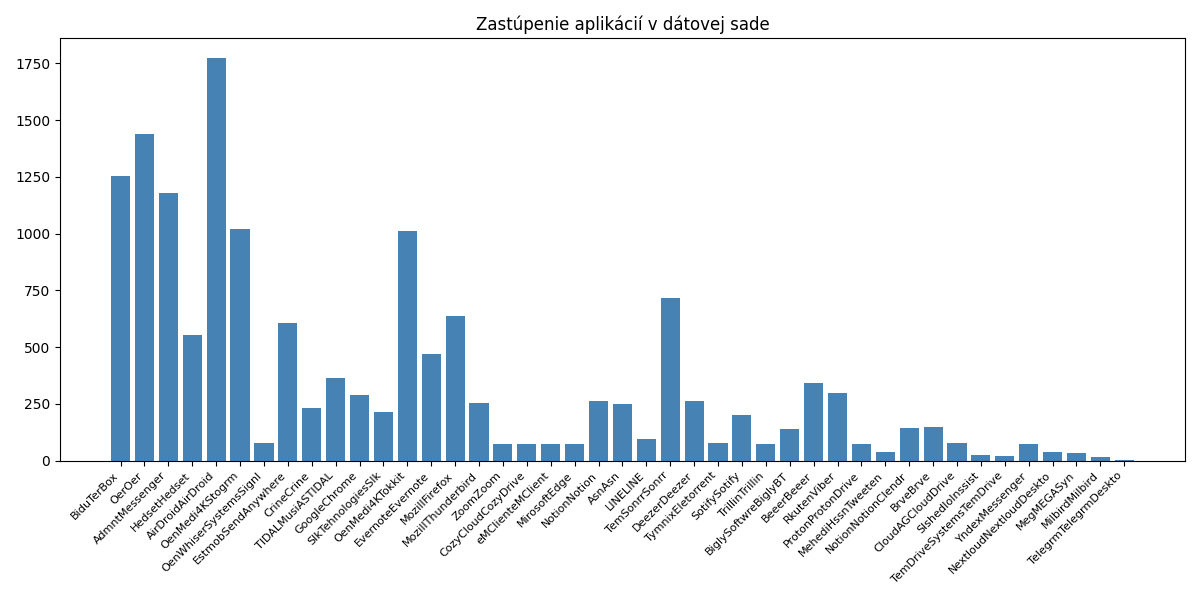
\includegraphics[width=1\linewidth]{obrazky-figures/all_apps_count_full.png}
    \caption{Grafické zobrazenie zastúpení jednotlivých aplikácií v dostupnej dátovej sade}
    \label{graph:all_apps_count}
\end{figure}
\newpage

%%%%%%%%%%%%%%%%%%%%%%%%%%%%%%%%%%%%%%%%%%%%%%%%%%%%%%%%%%%%%%%%%
%%%%%%%%%%%%%%%%%%%%%%%%%%%%%%%%%%%%%%%%%%%%%%%%%%%%%%%%%%%%%%%%%
%%%%%%%%%%%%%%%%%%%%%%%%%%%%%%%%%%%%%%%%%%%%%%%%%%%%%%%%%%%%%%%%%%%%%%%%%%%%%%%%%%%%%%%%%%%%%%%%%%%%%%%%%%%%%%%%%%%%%%%%%%%%%%%%%%

\begin{longtable}{lc}
\caption{Štatistický prehľad unikátnych hodnôt v datasete} \label{tab:unique_entries} \\
\toprule
\textbf{Parameter} & \textbf{Unikátne záznamy} \\ \midrule
\endfirsthead

\multicolumn{2}{c}%
{{\bfseries \tablename\ \thetable{} -- pokračovanie z predchádzajúcej strany}} \\
\toprule
\textbf{Parameter} & \textbf{Unikátne záznamy} \\ \midrule
\endhead

\midrule
\multicolumn{2}{r}{{Pokračuje na ďalšej strane...}} \\
\bottomrule
\endfoot

\bottomrule
\endlastfoot

SrcIP & 1252 \\
DstIP & 892 \\
SrcPort & 822 \\
DstPort & 2 \\
Proto & 1 \\
SNI & 306 \\
OrgName & 109 \\
TLS Version & 1 \\
Client CipherSuite & 14 \\
Client Extensions & 29 \\
Client Supported Groups & 39 \\
EC\_fmt & 2 \\
ALPN & 3 \\
Signature Algorithms & 10 \\
Client Supported Versions & 35 \\
JA3hash & 9415 \\
JA4 hash & 39 \\
JA4\_raw & 39 \\
Type & 3 \\
Server CipherSuite & 9 \\
Server Extensions & 42 \\
Server Supported Versions & 2 \\
JA3S hash & 58 \\
JA4S hash & 60 \\
JA4S\_raw & 60 \\
Version & 2 \\
\end{longtable}

\newpage


\chapter{Prehľad parametrov TLS \textit{Client Hello} správy}
V nasledujúcom zozname je uvedená ukážka štruktúry správy pre extrahované a sformátované vstupné dáta v dostupnom datasete.
\begin{lstlisting}[caption={Ukážka extrahovaných parametrov pre aplikáciu AirDroid}, label={lst:tls_airdroid}]
SrcIP: 172.17.151.209
DstIP: 65.9.95.47
SrcPort: 49751
DstPort: 443
Proto: 6
SNI: img-5-cdn.airdroid.com
OrgName: Amazon.com, Inc., AMAZO-CF
TLS Version: 771
Client CipherSuite: 47-53-156-157-4865-4866-4867-49171-49172-49195-49196-49199-49200-52392-52393
Client Extensions: 0-5-10-11-13-16-18-23-27-35-43-45-51-17513-65037-65281
Client Supported Groups: 0x0017,0x0018,0x001d,0x6399,0x9a9a
ALPN: h2,http/1.1
JA3hash: f9bb5c4d99971efe404e4722def23540
JA4 hash: t13d1516h2_8daaf6152771_02713d6af862
\end{lstlisting}

\chapter{Porovnanie funkčnosti referenčného a upravneného kódovania čisel portov}
V nasledujúcej tabuľke porovnávame výstupy referenčného a upraveného algoritmu s normalizáciou pre kódovanie čisel portov, ktorý bol optimalizovaný na zvýšenie váhy vyšších cifier pri súčasnom zachovaní významu nižších poradových čísel portov.
\begin{table}[H]
    \centering
    \caption{Porovnanie výstupov starého a nového algoritmu pre PortEmbedder triedu}
    \label{tab:port_comparison}
    \begin{tabular}{@{}rrr@{}}
        \toprule
        \textbf{Port} & \textbf{Starý algoritmus} & \textbf{Nový algoritmus} \\ \midrule
        420   & 0.1906202723 & 0.0023615173 \\
        10000 & 0.1210287443 & 0.1627282601 \\
        19999 & 0.6248108926 & 0.2052919290 \\
        20000 & 0.2420574887 & 0.3254565203 \\
        49999 & 0.9878971256 & 0.6934767094 \\
        50000 & 0.6051437216 & 0.8136413007 \\
        55245 & 0.8456883510 & 0.8367857548 \\
        60000 & 0.7261724660 & 0.9763695608 \\
        65535 & 1.0000000000 & 1.0000000000 \\ \bottomrule
    \end{tabular}
\end{table}
\enlargethispage{\baselineskip}

\chapter{Schéma implementácie systému}
\begin{figure}[H]
    \centering
    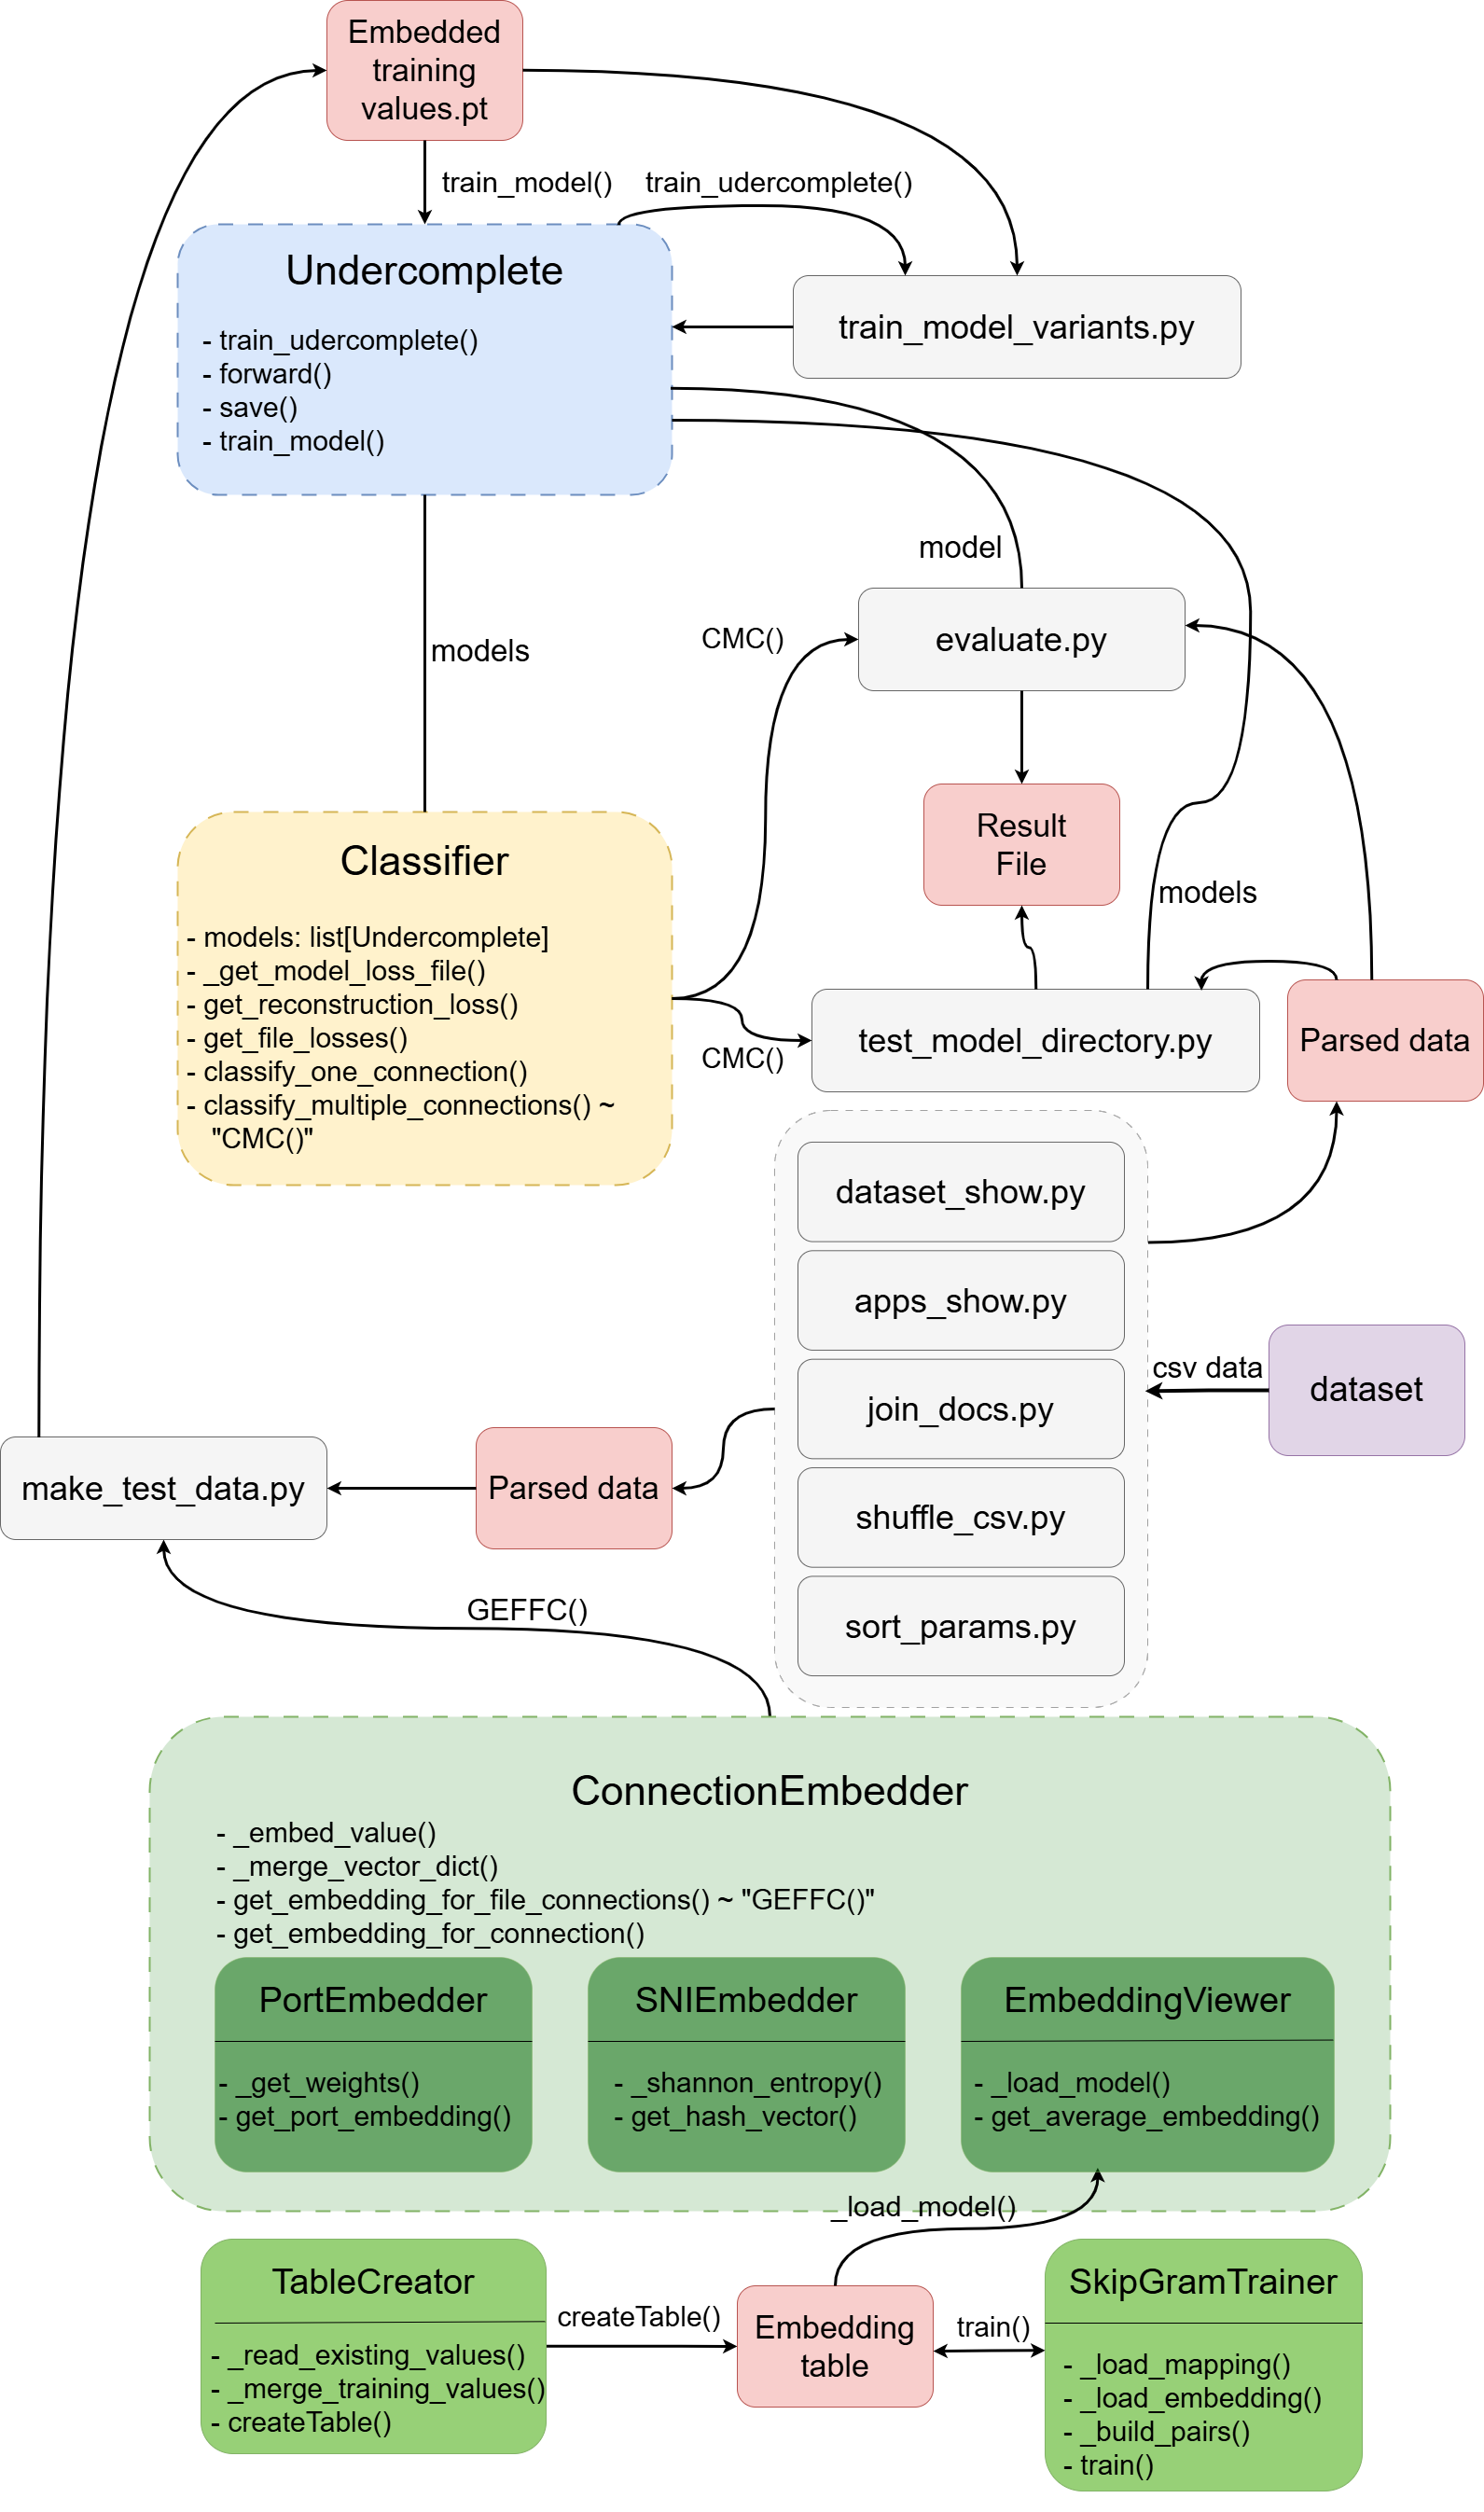
\includegraphics[width=0.59\linewidth]{obrazky-figures/CodeStruct.png}
    \caption{Schéma zobrazujúca skripty a~triedy implementovaného systému.}
    \label{fig:code_struct}
\end{figure}

\chapter{Grafy testovania rôzneho počtu vrstiev modelov}\label{append:layers_structs_graph}
V tejto časti sú graficky zobrazené výsledky testov rôznych štruktúr pre modely aplikácii AirDroid, BiduTerBox, Oer a AdmntMessenger. Na ose x sa celkové nachádzajú počty vrstiev modelu (tzn. skryté vrstvy so vstupnou a výstupnou vrstvou). Úspešnosť modelu je hodnotená MCC koeficientom, pričom sa berie ohľad aj na počet epoch, počas ktorých sa model trénoval, ktorých je definovaný konfiguráciou \textit{early stoppingu} (sekcia~\ref{exp:dynamic_delta})

\begin{figure}[H]
    \centering
    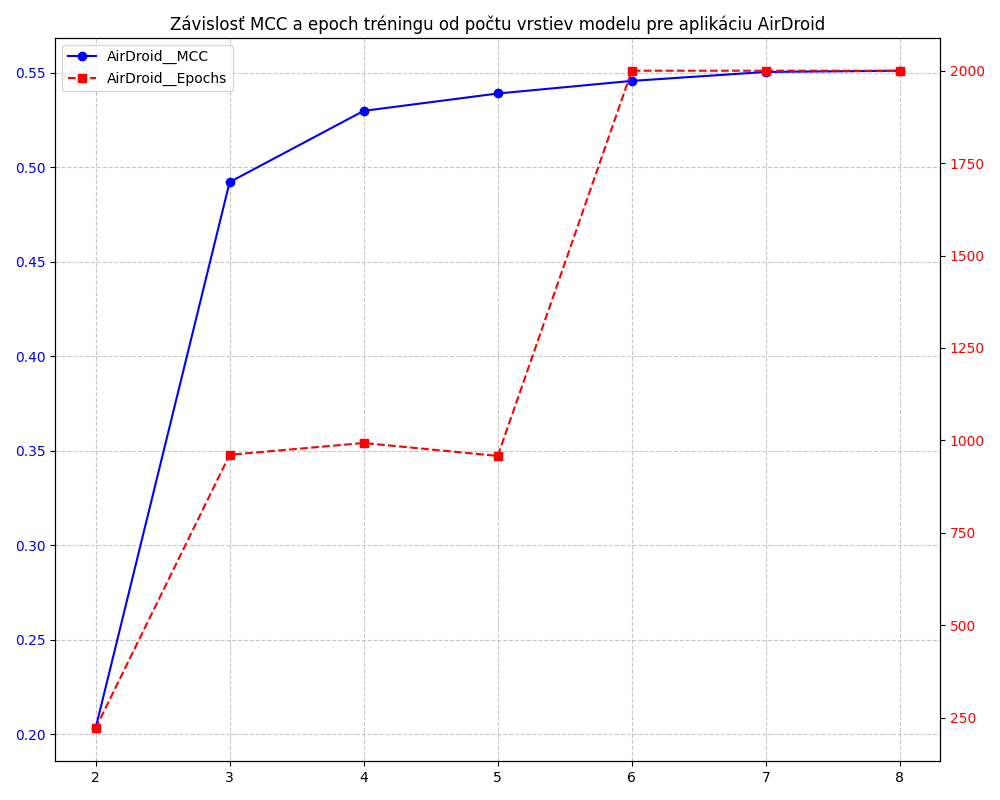
\includegraphics[width=0.75\linewidth]{obrazky-figures/AirDroidMCC.png}
    \caption{Porovnanie vplyvu počtu vrstiev na metriku MCC pre aplikáciu AirDroid.}
    \label{graph:AirDroidLayers}
\end{figure}

\begin{figure}[H]
    \centering
    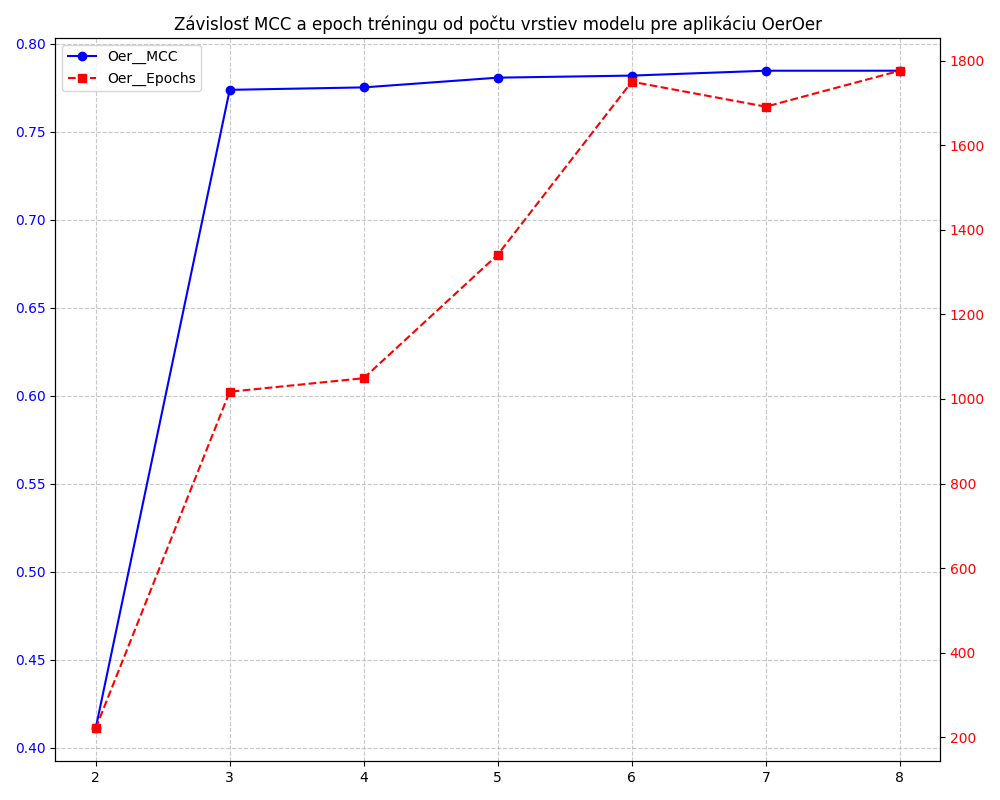
\includegraphics[width=0.75\linewidth]{obrazky-figures/OerMCC.png}
    \caption{Porovnanie vplyvu počtu vrstiev na metriku MCC pre aplikáciu Oer.}
    \label{graph:OerLayers}
\end{figure}

\begin{figure}[H]
    \centering
    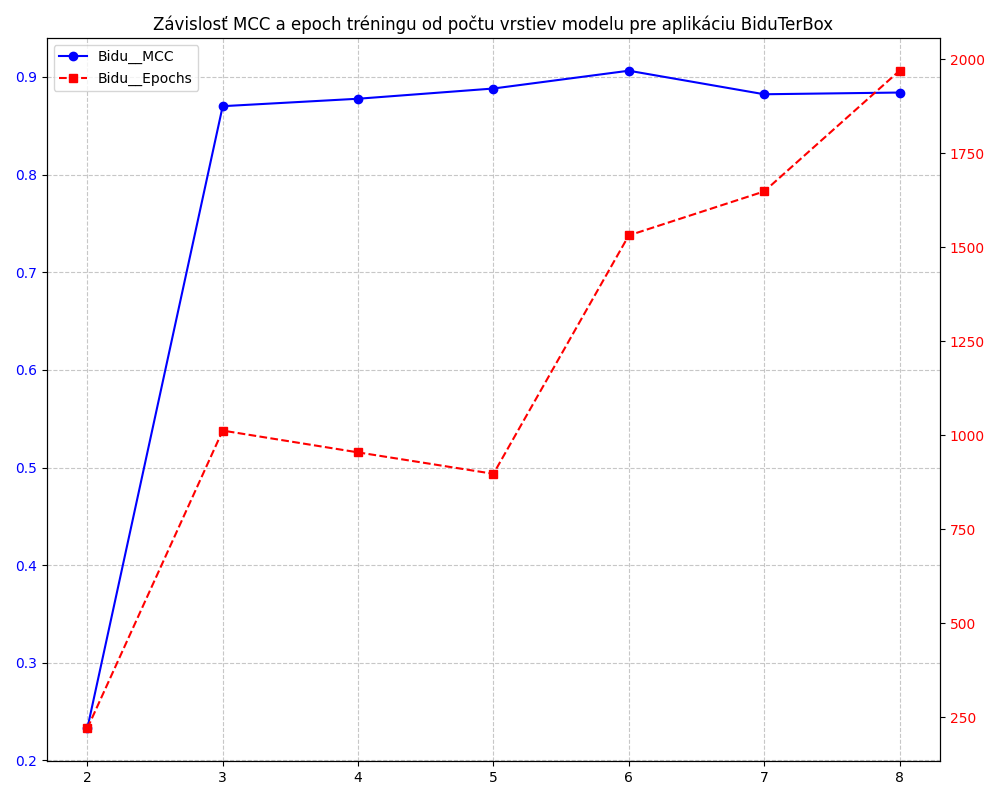
\includegraphics[width=0.75\linewidth]{obrazky-figures/BiduMCC.png}
    \caption{Porovnanie vplyvu počtu vrstiev na metriku MCC pre aplikáciu BiduTerBox.}
    \label{graph:BiduLayers}
\end{figure}

\begin{figure}[H]
    \centering
    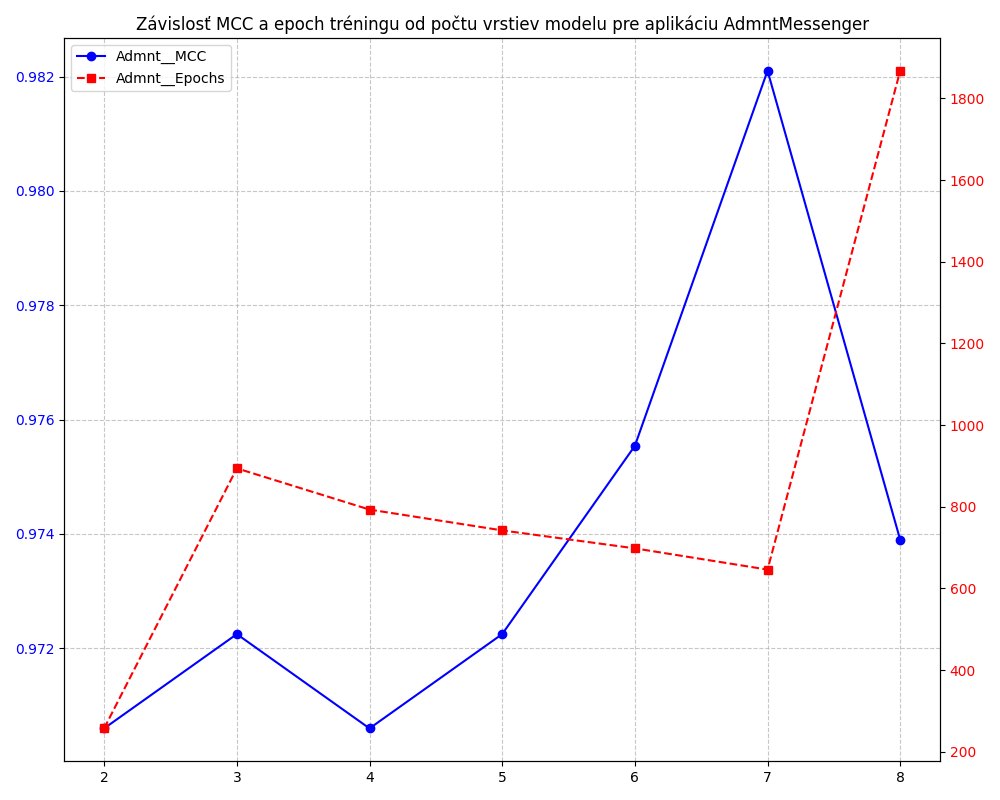
\includegraphics[width=0.75\linewidth]{obrazky-figures/AdmntMCC.png}
    \caption{Porovnanie vplyvu počtu vrstiev na metriku MCC pre aplikáciu AdmntMessenger.}
    \label{graph:AdmntLayers}
\end{figure}

\chapter{Grafy testovania rôznej veľkosti latentného priestoru modelu pre jednu cieľovú aplikáciu}
V tejto časti sú uvedené graficky zobrazené výsledky testov pre modely cieľovej aplikácie AirDroid, pričom každý model obsahuje rôznu dimenziu latentnej vrstvy (zobrazené na osi~x). 

\section{Grafy zobrazujúce závislosť MCC a počtu epoch pre trénovanie modelov od veľkosti latentnej vrstvy}\label{graph:latent_size_graphs}
% --- 4-layers
\begin{figure}[H]
    \centering
    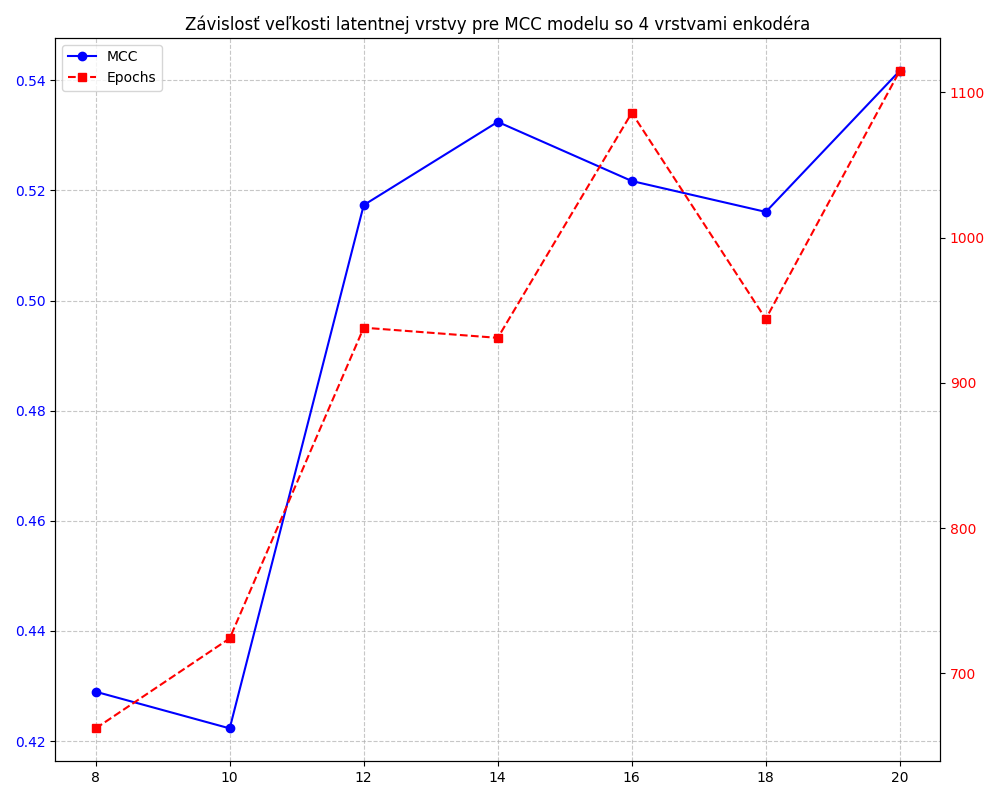
\includegraphics[width=0.75\linewidth]{obrazky-figures/Latent4.png}
    \caption{Vplyv veľkosti bottlenecku na MCC koeficient (4-vrstvový model).}
    \label{graph:Latent4MCC}
\end{figure}

\begin{figure}[H]
    \centering
    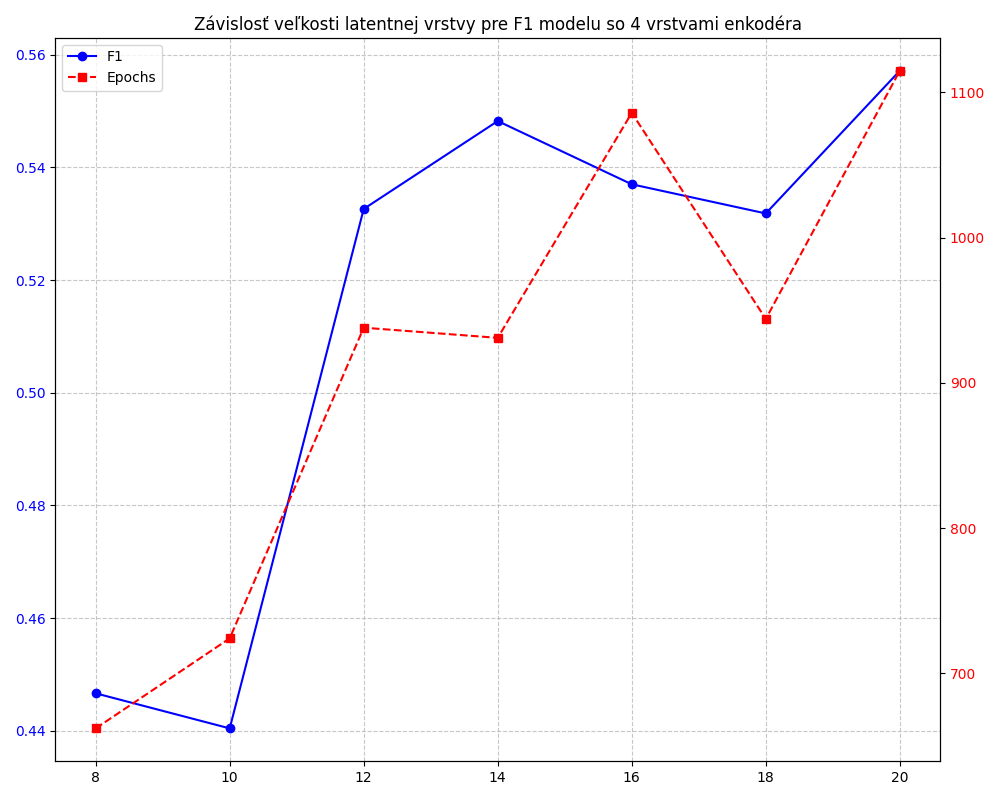
\includegraphics[width=0.75\linewidth]{obrazky-figures/Latent4F1.png}
    \caption{Vplyv veľkosti bottlenecku na F1 skóre (4-vrstvový model).}
    \label{graph:Latent4F1}
\end{figure}

% --- 5-layers
\begin{figure}[H]
    \centering
    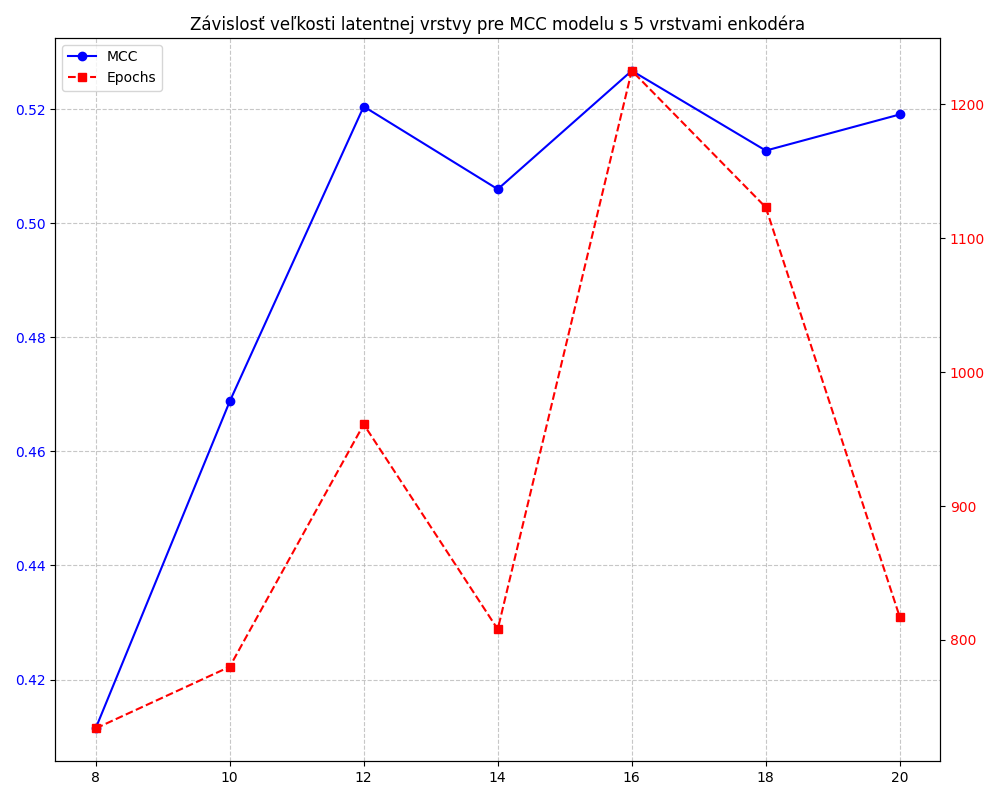
\includegraphics[width=0.75\linewidth]{obrazky-figures/Latent5.png}
    \caption{Vplyv veľkosti bottlenecku na MCC koeficient (5-vrstvový model).}
    \label{graph:Latent5MCC}
\end{figure}

\begin{figure}[H]
    \centering
    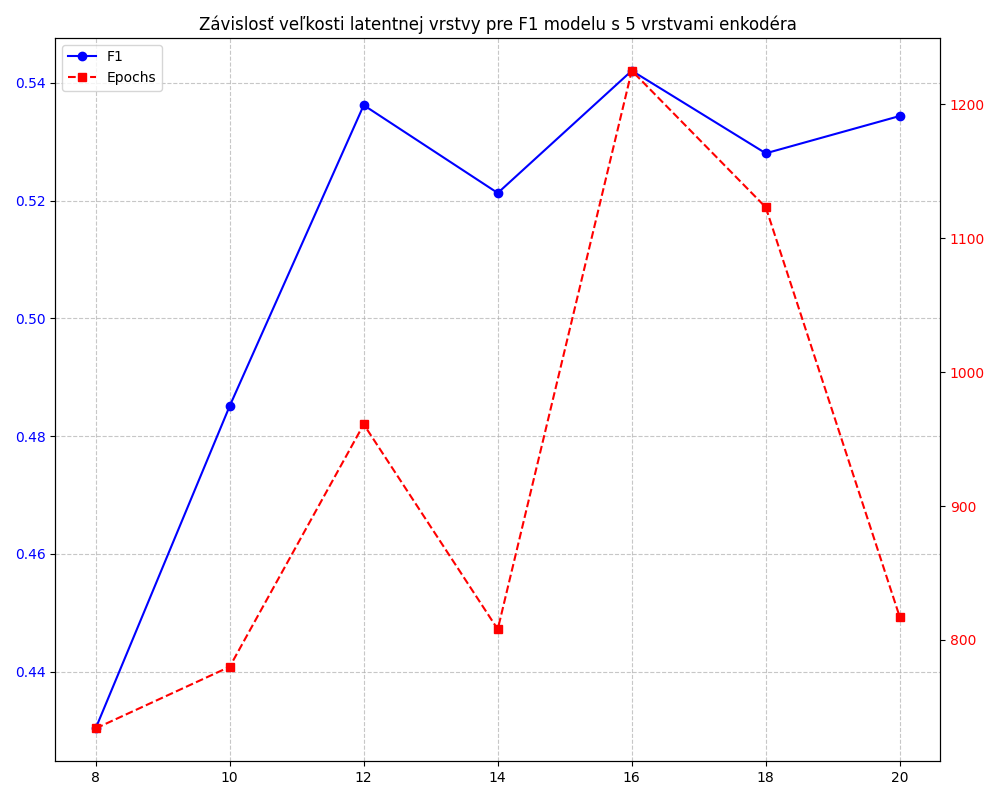
\includegraphics[width=0.75\linewidth]{obrazky-figures/Latent5F1.png}
    \caption{Vplyv veľkosti bottlenecku na F1 skóre (5-vrstvový model).}
    \label{graph:Latent5F1}
\end{figure}

% --- 6-layers
\begin{figure}[H]
    \centering
    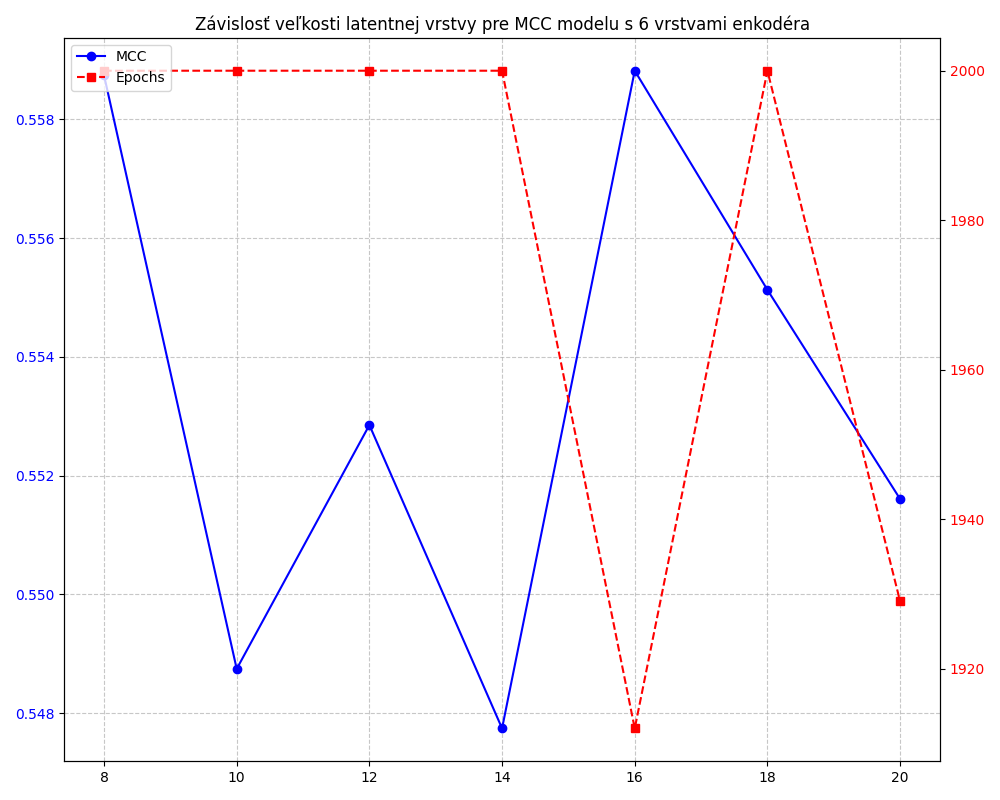
\includegraphics[width=0.75\linewidth]{obrazky-figures/Latent6.png}
    \caption{Vplyv veľkosti bottlenecku na MCC koeficient (6-vrstvový model).}
    \label{graph:Latent6MCC}
\end{figure}

\begin{figure}[H]
    \centering
    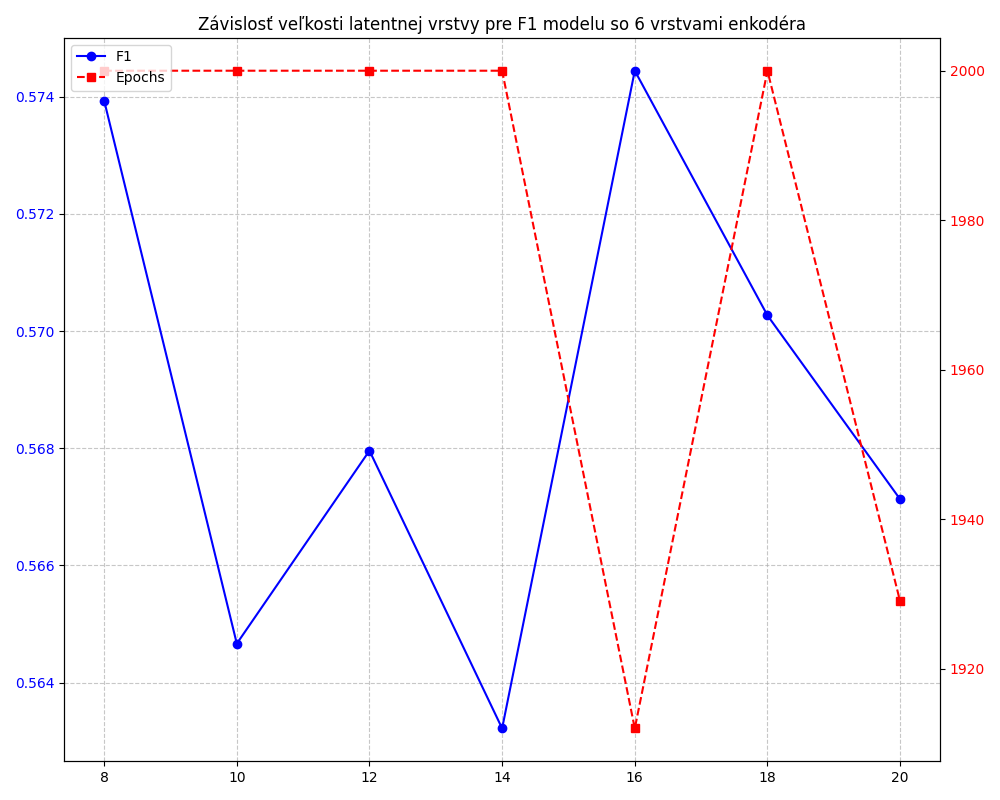
\includegraphics[width=0.75\linewidth]{obrazky-figures/Latent6F1.png}
    \caption{Vplyv veľkosti bottlenecku na F1 skóre (6-vrstvový model).}
    \label{graph:Latent6F1}
\end{figure}


\section{Grafy zobrazujúce závislosť Precision a Recall pre trénovanie modelov od veľkosti latentnej vrstvy}\label{graph:latent_size_graphs_Precision}

\begin{figure}[H]
    \centering
    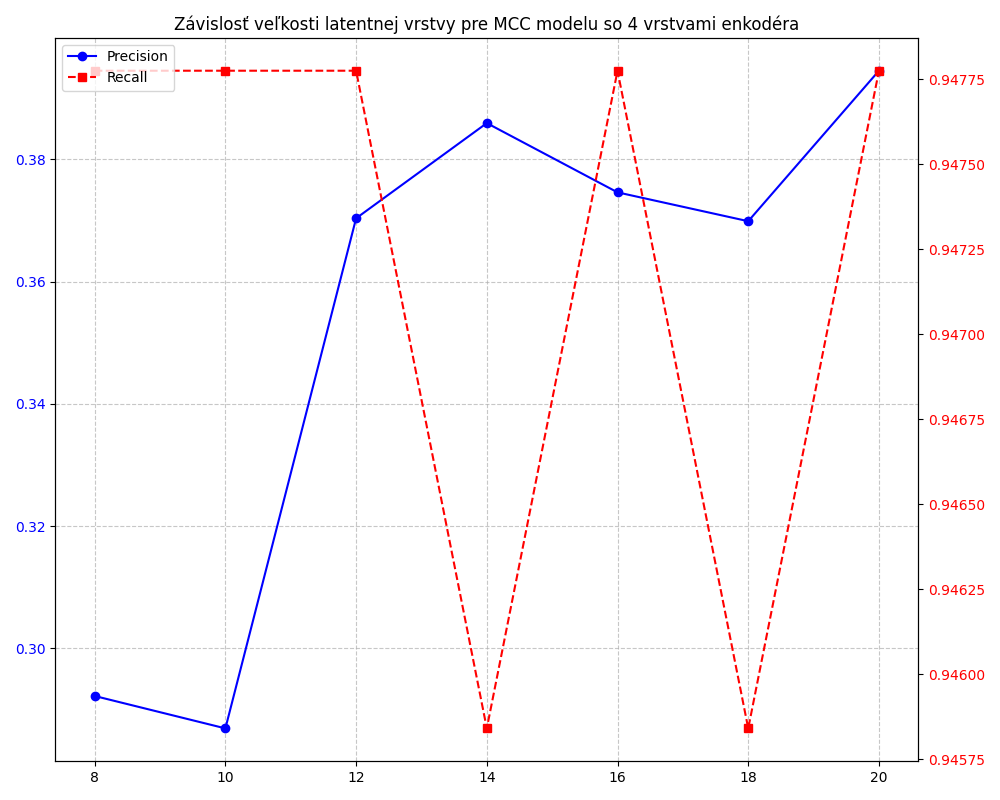
\includegraphics[width=0.75\linewidth]{obrazky-figures/PrecisionRecall4.png}
    \caption{Graf pre model obsahujúci 4 vrstvy v enkodéri.}
    \label{graph:LayersAirDroidPrecision4}
\end{figure}
\begin{figure}[H]
    \centering
    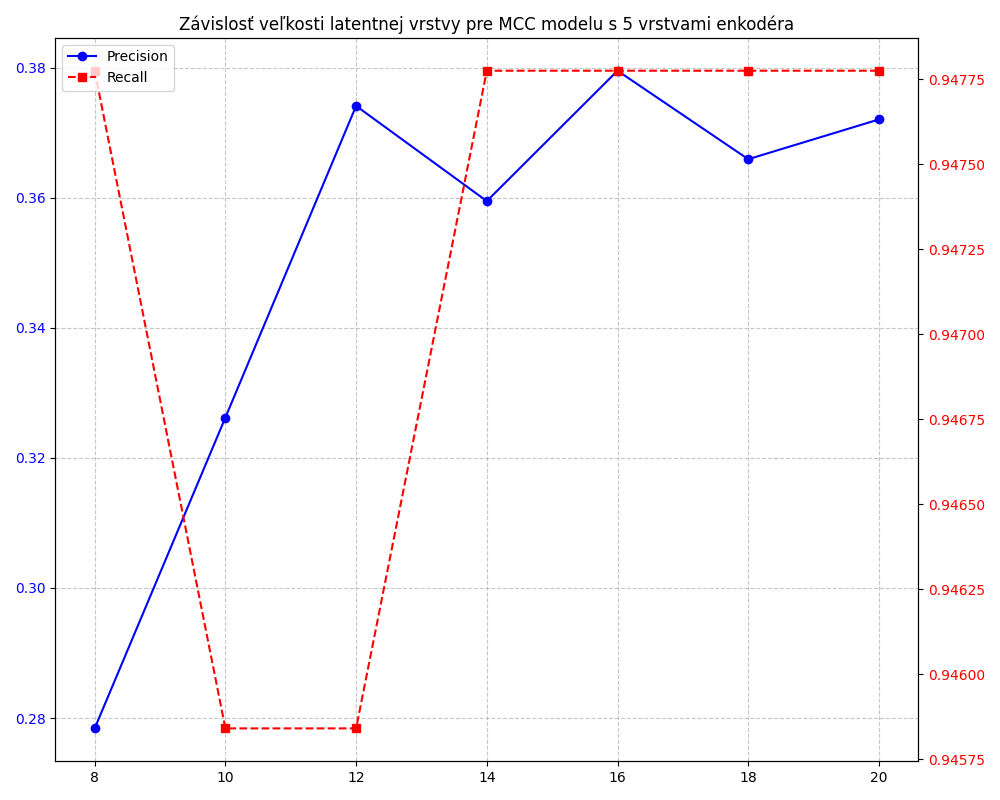
\includegraphics[width=0.75\linewidth]{obrazky-figures/PrecisionRecall5.png}
    \caption{Graf pre model obsahujúci 5 vrstiev v enkodéri.}
    \label{graph:LayersAirDroidPrecision5}
\end{figure}
\begin{figure}[H]
    \centering
    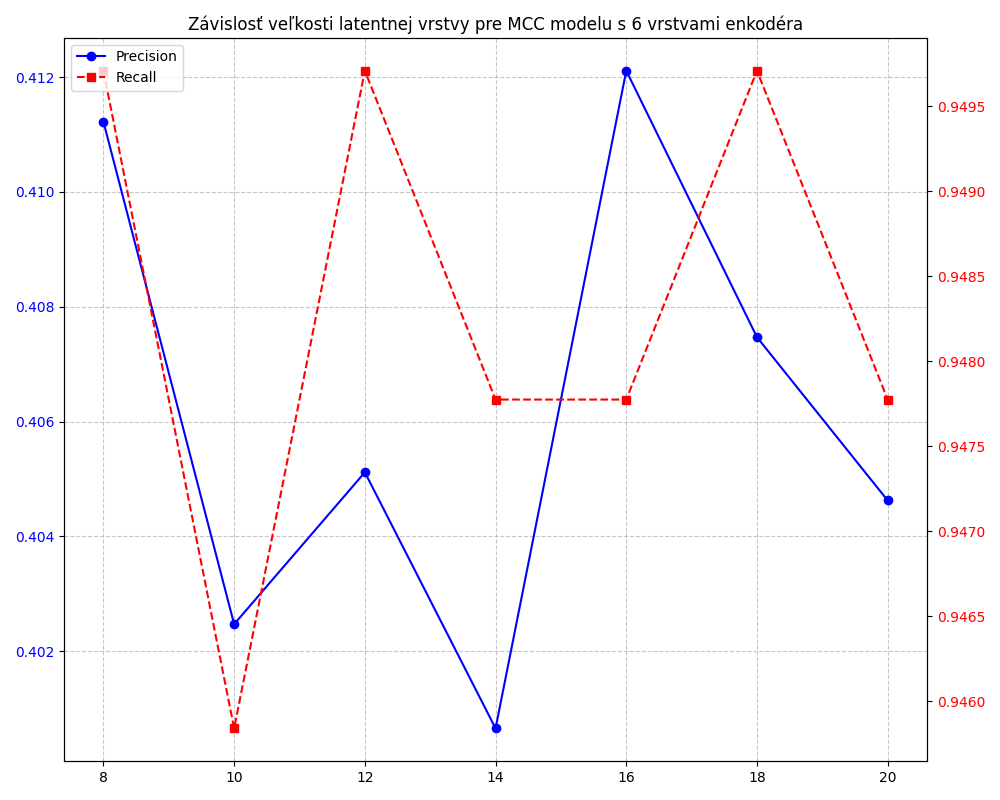
\includegraphics[width=0.75\linewidth]{obrazky-figures/PrecisionRecall6.png}
    \caption{Graf pre model obsahujúci 6 vrstiev v enkodéri.}
    \label{graph:LayersAirDroidPrecision6}
\end{figure}

\chapter{Štatistické výsledky modelov aplikácií}
V tejto časti sú uvedené metriky pre päť vybraných modelov, ktoré boli trénované a testované v rámci systému binárnej klasifikácie pre detekciu konkrétnych aplikácií.

\begin{table}[H]
    \centering
    \caption{Komplexné výsledky binárnej klasifikácie pre jednotlivé modely aplikácií.}
    \label{tab:each_model_all_metrics}
    \small
    \begin{tabular}{lrrrrr}
        \toprule
        \textbf{Metrika} & \textbf{AirDroid} & \textbf{BiduTerBox} & \textbf{OerOer} & \textbf{AdmntMsg} & \textbf{OenMedi4K} \\
        \midrule
        Accuracy [\%]    & 83,96    & 99,06    & 94,63    & 99,30    & 84,89    \\
        Precision        & 0,418    & 0,998    & 0,662    & 1,000    & 0,301    \\
        Recall           & 0,929    & 0,888    & 0,893    & 0,911    & 0,934    \\
        Specificity      & 0,828    & 1,000    & 0,952    & 1,000    & 0,843    \\
        FPR              & 0,172    & 0,000    & 0,048    & 0,000    & 0,157    \\
        F1 Score         & 0,577    & 0,940    & 0,761    & 0,953    & 0,456    \\
        MCC              & 0,555    & 0,937    & 0,741    & 0,951    & 0,479    \\
        \midrule
        Epochy           & 1124     & 1009     & 962      & 1100     & 1158     \\
        Čas tréningu [s] & 15,24    & 14,23    & 11,11    & 13,19    & 12,52    \\
        Chyba testu      & 0,00175  & 0,00109  & 0,00112  & 0,00093  & 0,00111  \\
        Prah             & 0,00296  & 0,00188  & 0,00217  & 0,00165  & 0,00167  \\
        \bottomrule
    \end{tabular}
\end{table}
  \fi
  
  % Kompilace po částech (viz výše, nutno odkomentovat)
  % Compilation piecewise (see above, it is necessary to uncomment it)
  % \subfile{projekt-30-prilohy-appendices}
  
\end{document}
